\documentclass[a4paper,12pt]{article}
\usepackage{pgfplotstable}
\usepackage{longtable}
\usepackage{varwidth}
\usepackage{array}
\usepackage{lscape}
\usepackage[top=4.5 cm,bottom=2.54cm, lmargin=2cm, rmargin=1.74cm, headheight=3.25cm]{geometry}
\usepackage{tabto}
\usepackage{collcell}
\usepackage{seqsplit}
\usepackage{fancyhdr}
\usepackage{lastpage}
\usepackage{xcolor}
\usepackage{sectsty}
\usepackage{mdframed}
% \usepackage{draftwatermark}
\usepackage{textpos}
\usepackage{placeins}
\usepackage{listings}
\usepackage{tikz}
\usepackage[hidelinks]{hyperref}
\usepackage{changepage}
\usepackage{float}
\usepackage{pdfpages}
\usepackage{fontspec}
\setmainfont{Calibri}
\setsansfont{Calibri}
%\SetWatermarkText{Draft}

\definecolor{maroon}{RGB}{122,11,44}
\sectionfont{\color{maroon}}  % sets colour of section headings

\definecolor{maroon_banner}{RGB}{141,28,59}

\renewcommand{\familydefault}{\sfdefault}

% Set title etc
\title {Copernicus Climate Change Service - 311a Lot 2 \\ Defining a Common Data Model}
\author {David I. Berry \\ National Oceanography Centre, UK}
\date{\today}

% empty header style for tables later on
\pgfplotstableset{
empty header/.style={
           typeset cell/.append code={%
               \ifnum\pgfplotstablerow=-1 %
                   \pgfkeyssetvalue{/pgfplots/table/@cell content}{}%
               \fi
           }
       }
   }

% new column for tables to split long strings
\newcolumntype{n}[1]{  > {\collectcell\seqsplit} V{#1} < {\endcollectcell}    }

% no indent of new paragraphs
\setlength{\parindent}{0pt}

% framed text boxes
\newcounter{FramedDepth}
\setcounter{FramedDepth}{-1}
\mdfdefinestyle{Framed}{linecolor=black,linewidth=1pt,leftmargin=10pt,rightmargin=10pt,
                        innerleftmargin=10pt,innerrightmargin=10pt}
\newenvironment{Framed}{%
  \addtocounter{FramedDepth}{1}
  \ifcase\theFramedDepth\def\FrameColour{white!50}%
    \or\def\FrameColour{white!50}%
    \or\def\FrameColour{white!50}%
    \or\def\FrameColour{white!50}%
    \fi%
  \begin{mdframed}[style=Framed,backgroundcolor=\FrameColour]%
}{\end{mdframed}\addtocounter{FramedDepth}{-1}}

% 1.25 18.4, 1.7
% 0.65
% Copernicus logo on page 3 onwards needs to go at (18.4cm, 1.7cm from top left of page) size (0.9cm by 0.86 cm)

% headers and footers
\headheight 3.5 cm          
\headsep  0.5 cm

\lhead{\textcolor{maroon}{Copernicus Climate Change Service}\vskip 0.5 cm}
\rhead{\includegraphics{/Users/dyb/GitHub/common_data_model/png/c3s_logo_small.png} \vskip 0.3 cm}

\lfoot{C3S\_311A\_Lot2\_NUIM\_2017SC1 - Initial specification for CDM}
\cfoot{}
\rfoot{Page \textbf{\thepage}  of \textbf{\pageref{LastPage}} }

\pagestyle{fancy}

% Autogenerated, do not edit
\newcommand{\revisiondate}{2017-08-02}
\newcommand{\revision}{v0.5-1-gf823ca4}


\begin{document}\thispagestyle{empty}


% Cover sheet

% top banner
\begin{tikzpicture}[remember picture,overlay]
\draw ([yshift=-15.7mm]current page.north) node[inner sep=0] (a) {\includegraphics[width=\paperwidth]{/Users/dyb/GitHub/common_data_model/png/c3s_banner_top.png}};
\draw ([yshift=-25.7mm]current page.north) node[inner sep=0] (a) {
\includegraphics[width=62.8mm]{/Users/dyb/GitHub/common_data_model/png/copernicus_logo_large.png}};
\node[shift={(0 mm, -10mm)}]  at (current page.north)   {
{\fontsize{8}{9.6}\selectfont \color{white} ECMWF COPERNICUS REPORT }\\
};
\end{tikzpicture}

% top maroon bar
\begin{tikzpicture}[remember picture,overlay]
\draw ([yshift=-53.3 mm]current page.north) node[inner sep=0] (a) {
\includegraphics[width=\paperwidth]{/Users/dyb/GitHub/common_data_model/png/header_bar.png}};
\draw (17.75,-0.23) node {
\includegraphics{/Users/dyb/GitHub/common_data_model/png/logo_thermometer.png}};
\node at (2.5,-0.35)   {
    {\fontsize{12}{14.4} \fontspec{Verdana} \selectfont \color{white} Copernicus Climate Change Service}
};
%\draw[style=help lines] (-2.5,0) grid (30,10);
\end{tikzpicture}


% Document title: Common Data Model for in situ observations
% Contract / Lot title: C3S311a Lot 2: Global Land and Marine Observations database
% Issued by: NUIM / Peter Thorne
% Date: DD/MM/YYYY
% C3S_D311a_Lot2.2.1.1_201708_CDM_Definition_v1


\vskip 4cm
\begin{adjustwidth}{2.5cm}{}
\fontsize{22}{26}\selectfont{
    \textbf{Common Data Model for in situ observations}\\
}
\fontsize{20}{24}\selectfont{
\textbf{\textcolor{maroon}{ C3S311a Lot 2: Global Land and Marine Observations Database } }\\
}

\vskip 5cm
\fontsize{12}{14}\selectfont{
\textbf{Issued by:} NUIM / Peter Thorne\\
\textbf{Date:} 21/08/2017\\
\textbf{Ref:} C3S\_D311a\_Lot2.2.1.1\_201708\_Initial\_specification\_for\_CDM\_v1\\
\textbf{Official reference number service contract:} 2017/C3S\_311a\_Lot2\_NUIM/SC1\\
}
\end{adjustwidth}

%footer bar
\begin{tikzpicture}[remember picture,overlay]
\draw ([yshift=15. mm]current page.south) node[inner sep=0] (a) {
\includegraphics[width=\paperwidth]{/Users/dyb/GitHub/common_data_model/png/footer_bar.png}};
\draw ([yshift=10.5 mm]current page.south) node[inner sep=0] (a) {\includegraphics{/Users/dyb/GitHub/common_data_model/png/copernicus_logo.png}};
\draw ([xshift=-30 mm, yshift=10.5 mm]current page.south east) node[inner sep=0] (a) {\includegraphics{/Users/dyb/GitHub/common_data_model/png/ECMWF_logo.png}};
\draw ([xshift=30 mm, yshift=10.5 mm]current page.south west) node[inner sep=0] (a) {\includegraphics{/Users/dyb/GitHub/common_data_model/png/ec_logo_small.png}};
\end{tikzpicture}
\newpage

\vspace*{\fill}
\begin{Framed}
\fontsize{9}{11}\selectfont
This document has been produced in the context of the Copernicus Climate Change Service (C3S).\\
The activities leading to these results have been contracted by the European Centre for Medium-Range Weather Forecasts, operator of C3S on behalf of the European Union (Delegation Agreement signed on 11/11/2014). All information in this document is provided "as is" and no guarantee or warranty is given that the information is fit for any particular purpose.\\
The user thereof uses the information at its sole risk and liability. For the avoidance of all doubts, the European Commission
and the European Centre for Medium-Range Weather Forecasts has no liability in respect of this document, which is merely representing the authors view.
\end{Framed}



% ========================= contributors page ===================================
% title page
\newpage

\begin{adjustwidth}{2.cm}{}
\vspace* {10mm}

{\fontsize{20}{24} \selectfont \textcolor{maroon}{Contributors}}\\

{\fontsize{14}{17} \selectfont \textbf{\uppercase{{National Oceanography Centre (NOC), Natural Environment Research Council (NERC)}}}}
\begin{enumerate}
\item David I. Berry (Lot 2)
\item Elizabeth C. Kent (Lot 2)\\
\end{enumerate}


{\fontsize{14}{17} \selectfont \textbf{\uppercase{Istituto di Metodologie per l'Analisi Ambientale (IMAA), Consiglio Nazionale delle Ricerche (CNR)}}}
\begin{enumerate}
\item Fabio Madonna (Lot 3)
\item Emanuele Tramutola (Lot 3)
% \item Ermann Ripepi (Lot 3)
\end{enumerate}

{\fontsize{14}{17} \selectfont \textbf{\uppercase{Instituto Dom Luiz, Universidade de Lisboa}}}
\begin{enumerate}
\item Maria Ant\'onia Valente (Lot 1)\\
\end{enumerate}

{\fontsize{14}{17} \selectfont \textbf{\uppercase{Universitat Rovira i Virgili }}}
\begin{enumerate}
\item Alba Gilabert Gallart (Lot 1)
\item Manola Brunet (Lot 1)\\
\end{enumerate}

{\fontsize{14}{17} \selectfont \textbf{\uppercase{Met Office}}}
\begin{enumerate}
\item Robert Dunn (Lot 2)
\item Philip Brohan (Lot 1)
\item Rob Allan (Lot 1)\\
\end{enumerate}

{\fontsize{14}{17} \selectfont \textbf{\uppercase{National University of Ireland Maynooth (NUIM)}}}
\begin{enumerate}
\item Peter Thorne (Lots 2 and 3)
\item Simon Noone (Lot 2)\\
% \item Anthony Kettle (Lot 2)
\end{enumerate}

{\fontsize{14}{17} \selectfont \textbf{\uppercase{Science Technology Facilities Council (STFC)}}}
\begin{enumerate}
\item Ag Stephens (Lot 2)\\
\end{enumerate}

{\fontsize{14}{17} \selectfont \textbf{\uppercase{Koninklijk Nederlands Meteorolgisch Instituut (KNMI)}}}
\begin{enumerate}
% \item Ge Verver (Lot 4)
\item Else van den Besselaar (Lot 4)
% \item Wim Som de Cerff (Lot 4)
% \item Maarten Plieger (Lot 4)
\end{enumerate}

\end{adjustwidth}


% ========================= Executive summary ===================================
%\maketitle
\newpage

\section*{Executive Summary}
This document defines the initial version of the Common Data Model (CDM) developed within the Copernicus Climate Change Service (C3S) Access to Global Land and Marine Observations Database (C3S 311a Lot 2) service. This has been developed in consultation across the four C3S 311a (Collection and Processing of In Situ Observations) Lots and ECMWF.\\

Tab separated versions of the code tables defining the data model can be found at:\\ \\
\tabto{2cm} \url{https://github.com/glamod/common_data_model/tree/master/tables/}

\begin{table}[H]
\centering
\begin{tabular}{|c|c|l|}
\hline
\textbf{Version} & \textbf{Release date} & \textbf{Release notes}\\
\hline
1 & 31/08/2017 & Initial version of the common data model\\
1.01 & 12/09/2017 & 'sub\_region' table updated\\
1.02 & 13/10/2017 & Updates to a number of tables to fix broken references\\
\hline
\end{tabular}
\end{table}
% Revision number: \revision \\
% Revision date: \revisiondate \\

\newpage
\tableofcontents
\newpage
\listoftables
\newpage

% ================================= Introduction ======================
\section {Introduction}

\subsection {Purpose of this document}
This document defines the initial version of the Common Data Model (CDM)\footnote{As noted in the ITT: A common data model is different from a file format, which defines how information is encoded in a file. The purpose of a data model is to provide a well-defined data structure that can be used to represent data records from a variety of sources, in such a way that the information contained in those records can be unambiguously accessed using a common set of tools. Development of a common data model for observations involves specification of data attributes and their symbolic names, including, for example, identifiers for different instruments, observed parameters, geolocation and timing, etc. A governance structure is required to manage such specifications, ensure consistency with standards where they exist, and to ensure a controlled evolution of the data model.} developed within the Copernicus Climate Change Service (C3S) Access to Global Land and Marine Observations Database (C3S 311a Lot 2) service. This has been developed in consultation across the four C3S 311a (Collection and Processing of In Situ Observations) Lots and with ECMWF.

\subsection {Scope}
The defined common data model is intended for use with in situ land and marine observations. Instantaneous (or point) observations and temporal statistics (e.g. daily and monthly min / max temperatures, accumulation of precipitation etc.) are supported through the use of a significance qualifier. Similarly, column average data are supported through the reporting of the observed variable alongside its value. Profile data is supported through reporting the z-coordinate for each observed value.\\

Whilst initially intended for use with observations of Essential Climate Variables (ECVs; e.g. GCOS, 2016) the data model is not restricted to the ECVs. As noted above, and following the ECMWF Observations DataBase (ODB) type data model, the observed variable is reported alongside the observed value.\\

Comprehensive metadata is supported through the use of configuration tables, recording information on:
\begin{itemize}
\item Source level metadata: e.g. original source of data, source data centre, citation information etc.
\item Station level metadata: e.g. location, operating institute, parameters reported etc.
\item Profile level metadata: Additional information for profile data, e.g. unwinder type, type of balloon or expendable bathythermograph (XBT) etc.
\item Sensor level metadata: e.g. calibration history and status, sensor type / serial number etc.
\end{itemize}
Comprehensive quality control and uncertainty information can be recorded using linked Entity-Attribute-Value (EAV) tables.

\subsection {Structure of this document}

Section 2 of this document provides background information on the data model and existing relevant data models and standards. Section 3 proposes a governance mechanism for the CDM in recognition that the data model will change and evolve as the requirements of the users and the C3S Climate Data Store develop. Section 4 describes the core components and tables of the data model. The appendix includes the individual table definitions and preliminary versions of the code tables. The code tables listed are provisional and will be expanded as the service develops.

% =============================== background =========================
\section {Background and existing standards}
\subsection {Observational sources and requirements of the data model}

Across the C3S 311a service (Collection and Processing of In Situ Observations) access will be provided to observations from surface terrestrial and marine environments and upper air data in a common data model. The observations included range from point observations made from moving platforms to daily and monthly statistics at fixed locations. The parameters reported include, inter alia: air temperature; humidity; wind speed; pressure; cloud cover information; present weather. The statistics include, inter alia: daily min, max and mean air temperature; accumulated precipitation over 3 or 24 hours; mean wind speed over the preceding 10 minutes. The full range of parameters and statistics to be reported will evolve as the service is developed. As new parameters are recovered from newly digitised sources and the reprocessed climate archives the list of parameters will need to expand.\\

Both surface level (terrestrial and marine) and upper air data will be initially included in the service. The surface level data include observations made at standard and non-standard heights. The upper air data will include multiple observations, starting at the surface and at increasing heights through the atmosphere, often as a function of pressure or geopotential height. Columnar averages will be included. As a result the data model needs to include the flexibility to record the height and the units used for reporting the height of measurement with every observation. Similarly, some reporting stations, and hence observations, will move in the horizontal plane, and the horizontal coordinates need to be reported with each observation. To avoid ambiguity, the coordinate reference system (CRS) should be provided with each location reported.\\

The period covered by Lot 2 of the service ranges from $\sim$1850 to present. Over this period there have been many changes to the instruments and practices used to record the various parameters. The choice of instruments and practices will influence the quality of the observations and a change in instrumentation, or location, may introduce inhomogeneities into the record. To mitigate this risk comprehensive observational metadata are required. Similarly, information on adjustments and conversions applied to the data need to be recorded. The full range of observational practices and instruments used is not currently known and developed data model will need to be extendable to accommodate new metadata as required.\\

The observations to be included will be sourced from a variety of existing datasets, such as the International Comprehensive Ocean and Atmosphere Data Set (ICOADS; e.g. Freeman et al., 2017), and newly digitised sources. In defining the data model the provenance and lineage of the data sources need to be preserved. Similarly, usage rights and citation information need to be preserved and provided to users alongside the observational data. This is a common requirement across all Lots within the service.\\

In order to meet the above requirements a data model based on the ECMWF Observations DataBase (ODB) model has been developed, with the use of linked tables providing information on the observational and provenance metadata. The ODB type model allows for extension to new parameters through the use of a parameterized observation list (see next section). The linked tables will define a core set of parameters under 4 different categories (station, source, profile and sensor), flexibility will be provided through the specification of optional elements and associated decode tables.\\

\subsection{ECMWF Observations DataBase (ODB)}

The data model developed and used in the ECMWF Observations DataBase (ODB) software allows the representation of environmental data from many sources, including in situ observations and weather reports, satellite data and model output. As noted in Hersbach et al. (2015), in the ODB implementation a distinction is made between weather reports and observations and this same distinction is made within the CDM and this document.  A weather report, such as a ship weather report or a radiosonde ascent, may contain multiple observations of one or more parameters. In the case of a ship weather report observations of the air temperature and humidity, sea level pressure, sea surface temperature, wind speed and direction are typically made and recorded in a single report. In the case of a radiosonde report observations of the temperature will be made at a range of levels from the surface to the burst point of the balloon. To enable flexibility and scalability with the ODB data model the different elements making up a weather report are split into header elements, recording information common across a weather report, and observational (or body) elements specific to a single observation.\\

In the original version of ODB, e.g. Saarinen (2004), these elements were split between a header table, containing the header elements, and a linked body table containing the observations or body elements. Within the body table the name of the parameter being observed, or its numerical code, is recorded in one column and the observed value within a second column.  Other columns, recording information such as QC results, are permissible. This data model allows the efficient expansion of the data model to new variables, without the need to change the underlying structure, by the addition of the new variable to the enumerated list defining the reportable variables. Within the latest version of ODB (ODB-2; e.g. Hersbach et al., 2015) the header and body tables have been combined into a single flat table, with the header rows repeated, to enable efficient archival within the ECMWF MARS system. A simplified schematic of the ODB-2 structure is shown in Table 1.\\

Within the CDM defined in this document we have opted for the original ODB type data model, with the reports split into header and observational records stored within separate tables. These are described fully within Section 3 of this document. When these tables are stored in a relational database, or similar structure, performing a join on the tables should result in ODB-2 compatible records.\\


\pgfplotstabletypeset[
   empty header,
    begin table=\begin{longtable},
    %every head row/.style={output empty row},
    every nth row={1}{before row=\hline},
    every first row/.append style={
        before row={%
            % Initial caption
            \caption{Simplified example of records in ODB type data model, with observations from reports 1 and 2 spanning multiple records. For simplicity, the z coordinate has been omitted but profile data would be represented with each layer / height as a separate record}
            \label{tab:DataTableODB}\\
            % Initial column headers
            \hline\hline
            \multicolumn{5} {c} { \textbf{header information}} & 
            \multicolumn{3} {c} { \textbf{observation information}} 
            \\
            \hline
            \multicolumn{1} { > {\centering}V{0.3 in}} { \textbf{record id}} & 
            \multicolumn{1} { > {\centering}V{0.3 in}} { \textbf{report id}} & 
            \multicolumn{1} { > {\centering}V{0.3 in}} { \textbf{obs id}} & 
            \multicolumn{1} { > {\centering}V{1 in}} { \textbf{date}} & 
            \multicolumn{1} { > {\centering}V{1 in}} { \textbf{location}} & 
            \multicolumn{1} { > {\centering}V{0.75 in}} { \textbf{parameter}} & 
            \multicolumn{1} { > {\centering} V{0.75 in} } {\textbf{value}} &
            \multicolumn{1} { > {\centering} V{0.75 in} } {\textbf{units}} 
            \\ \hline\hline \endfirsthead
            \multicolumn{6}{c}{Table \thetable\ adjustment (cont.)} \\
            % column headers on additional pages
            \hline\hline 
            \multicolumn{5} { > {\centering}V{2.9 in}} { \textbf{header information}} & 
            \multicolumn{3} { > {\centering}V{2.25 in}} { \textbf{observation information}} 
            \\
            \hline
            \multicolumn{1} { > {\centering}V{0.3 in}} { \textbf{record id}} & 
            \multicolumn{1} { > {\centering}V{0.3 in}} { \textbf{report id}} & 
            \multicolumn{1} { > {\centering}V{0.3 in}} { \textbf{obs id}} & 
            \multicolumn{1} { > {\centering}V{1 in}} { \textbf{date}} & 
            \multicolumn{1} { > {\centering}V{1 in}} { \textbf{location}} & 
            \multicolumn{1} { > {\centering}V{0.75 in}} { \textbf{parameter}} & 
            \multicolumn{1} { > {\centering} V{0.75 in} } {\textbf{value}} &
            \multicolumn{1} { > {\centering} V{0.75 in} } {\textbf{units}} 
            \\ \hline\hline \endhead
            % Footer on 1st to penultimate pages
            \multicolumn{6}{r}{{Continued on next page}} \\
            \endfoot
            % Footer on last page of table
            \hline
            \multicolumn{6}{r}{{End of table}} \\ 
            \endlastfoot
        }
    },
    %
    end table=\end{longtable},
    col sep = &,
    row sep = \\ , 
    columns/record id/.style={string type, column type = V{0.3 in}},
    columns/report id/.style={string type, column type = V{0.3 in}},
    columns/observation id/.style={string type, column type = V{0.3 in}},
    columns/date/.style={string type, column type = V{1 in}},
    columns/location/.style={string type, column type = V{1 in}}, 
    columns/parameter/.style={string type, column type = V{1 in}},
    columns/value/.style={string type, column type = V{0.3 in}},
    columns/units/.style={string type, column type = V{0.3 in}}
]{
record id& report id& observation id& date & location & parameter & value & units \\
1 & 1 & 1 & 2012-01-01 12:00+0.0 & POINT(-40 40) & air temperature & 300.0 & K \\
2 & 1 & 2 & 2012-01-01 12:00+0.0 & POINT(-40 40) & sea level pressure & 1013.0 & hPa \\
3 & 2 & 3 & 2012-01-01 18:00+0.0 & POINT(-40.1 40.2) & air temperature & 300.3 & K \\
4 & 2 & 4 & 2012-01-01 18:00+0.0 & POINT(-40.1 40.2) & sea level pressure & 1013.2 & hPa \\
}


\subsection {BUFR and WIGOS Metadata Standard}
There has been a large body of work and significant effort invested in defining data models and parameterising the data and metadata for encoding the data into those data models.  Within the scope of the CDM and the C3S 311a service, the WMO Binary Universal Form for the Representation of meteorological data (BUFR) (WMO, 2015a) and the WMO Integrated Observing System Metadata Standard (WMDS) (WMO, 2015b) are key background material. \\

The BUFR format (WMO 2015a) is a flexible and efficient table driven format for reporting weather observations on the WMO Global Telecommunications System (GTS) in binary. The tables defined as part of the BUFR format include many of the parameters that will be included in the CDM. For example, Common code table C6 (WMO 2015a) includes all the measurement units reportable in BUFR (and other WMO codes). Similarly, code tables are defined for reporting instrument types and methods, station types etc. Where possible, these code tables have been referenced and used in preference to defining new code tables.  BUFR tables from Version 27 of Master Table 0 have been used in this version of this document.\\

In recognition of the increasing importance of observational metadata the WMDS is currently under development and phased implementation (WMO, 2015b). The WMDS extends the ISO19115 metadata standard, with additional mandatory elements describing both the station level and discovery metadata as well as specific information on the instrumentation used and processing steps. As part of the process simplified versions of BUFR and other tables have been included in the standard. As with BUFR these tables have been referenced, where appropriate, in preference to defining new code tables.

\section {Governance of the Common Data Model}
A working group will be set up to manage the governance of the common data model. This group will operate remotely via email and regular teleconferences.  Proposals to add new entries to the code tables or make changes to the structure of the common data model shall be made via email to email address:\\

\tabto{2cm} {c3s\_311a\_CDM\_governance}@surfacetemperatures.org.\\

Emails to this address will be distributed to all members of the working group. \\

During the initial development stage of the service proposals sent to the above email address will be assessed monthly, with discussion via email and teleconference as required. Accepted changes will be implemented at the beginning of the following month or with at least 2 weeks notice. These changes will be published both via the service website and via a subscription email list:\\

\tabto{2 cm} {c3s\_311a\_CDM\_notifications}@surfacetemperatures.org.\\

The working group will be self nominating and initially contain at least one member from each Lot to act as a primary point of contact for that Lot and to represent their requirements on the working group. The working group will also contain a representative from ECMWF, or a nominated representative from another organisation, to represent the needs of the wider C3S community. Additional members from the different Lots will be welcomed. In the case of disagreement over proposed changes each Lot will have one vote irrespective of the number of members in the working group. In the case of a hung vote ECMWF, or their representative, will have the deciding vote.\\

\section {Common Data Model}
As noted above, the CDM is based on the original ODB data model, with meteorological reports split into header and observational records stored in separate tables, header\_table and observations\_table respectively. In support of these two primary tables, four auxiliary tables have been defined to enable the comprehensive reporting of metadata at different levels:\\

\begin{itemize}
\item Source level metadata (\textit{source\_configuration} table). This level contains detailed information on the source dataset, including: information on the product; whether any processing has been applied; the original data centre the data were sourced from; citation information; the data licence for the product; how to cite the data source etc.
\item Station level metadata (\textit{station\_configuration} table). This level contains detailed information on the station reporting the data including: station operator; the type of station; station / AWS model type; location; operating territory; reporting frequency etc.
\item Profile level metadata (\textit{profile\_configuration} table). This level contains detailed metadata for atmospheric and oceanic profiles, including: profile type; type of launcher; direction of profile; balloon / XBT type etc.
\item Instrument (or sensor) level metadata (\textit{sensor\_configuration} table). This level contains detailed information on the sensor used to make a particular observation, including: calibration status; sampling strategy; observing method; sensor housing and ventilation; instrument model and serial number etc.
\end{itemize}

These tables are defined in the following section and contain elements that are mandatory across all report types. Additional optional elements are provided through Entity-Attribute-Value based tables linked to the configuration tables. Two additional tables have been defined to include the reporting of comprehensive uncertainty estimates and quality control flags. A simplified schematic of the 12 tables forming the core of the CDM is shown in Figure 1 - a more complete schematic can be found at \url{https://github.com/glamod/common_data_model/blob/master/cdm_full.pdf}. \\

Within the tables in the following sections the following syntax has been used:\\
\begin{itemize}
\item numeric \tabto{2 cm} Any numeric value (integer or floating point).
\item int \tabto{2 cm} An integer value.
\item varchar \tabto{2 cm} A variable length character string.
\item timestamp \tabto{2 cm} A timestamp with time zone, e.g. "2017-07-01 00:00:0.0+00".
\item {[]} \tabto{2 cm} An array of the indicated type.
\item {*} \tabto{2 cm} An optional element.
\item (pk) \tabto{2 cm} The indicated elements marked as (pk) within a table form the unique ID for the record.
\end {itemize}

Unless indicated otherwise all elements listed are mandatory but may be encoded as missing (e.g NA, NULL or format specific equivalent) if not available. Optional elements are indicated by *. Whilst arrays have been indicated for the elements containing multiple values this does not preclude other implementations. Within the table definitions references to external tables are indicated in the external\_table column. These references are composed of two parts separated by a colon (:). The first part indicates the table, the second the element within the table. For example, station\_configuration:primary\_id indicates a reference to the primary\_id element in the station\_configuration table.\\

\begin{landscape}
\begin{figure}
\centering
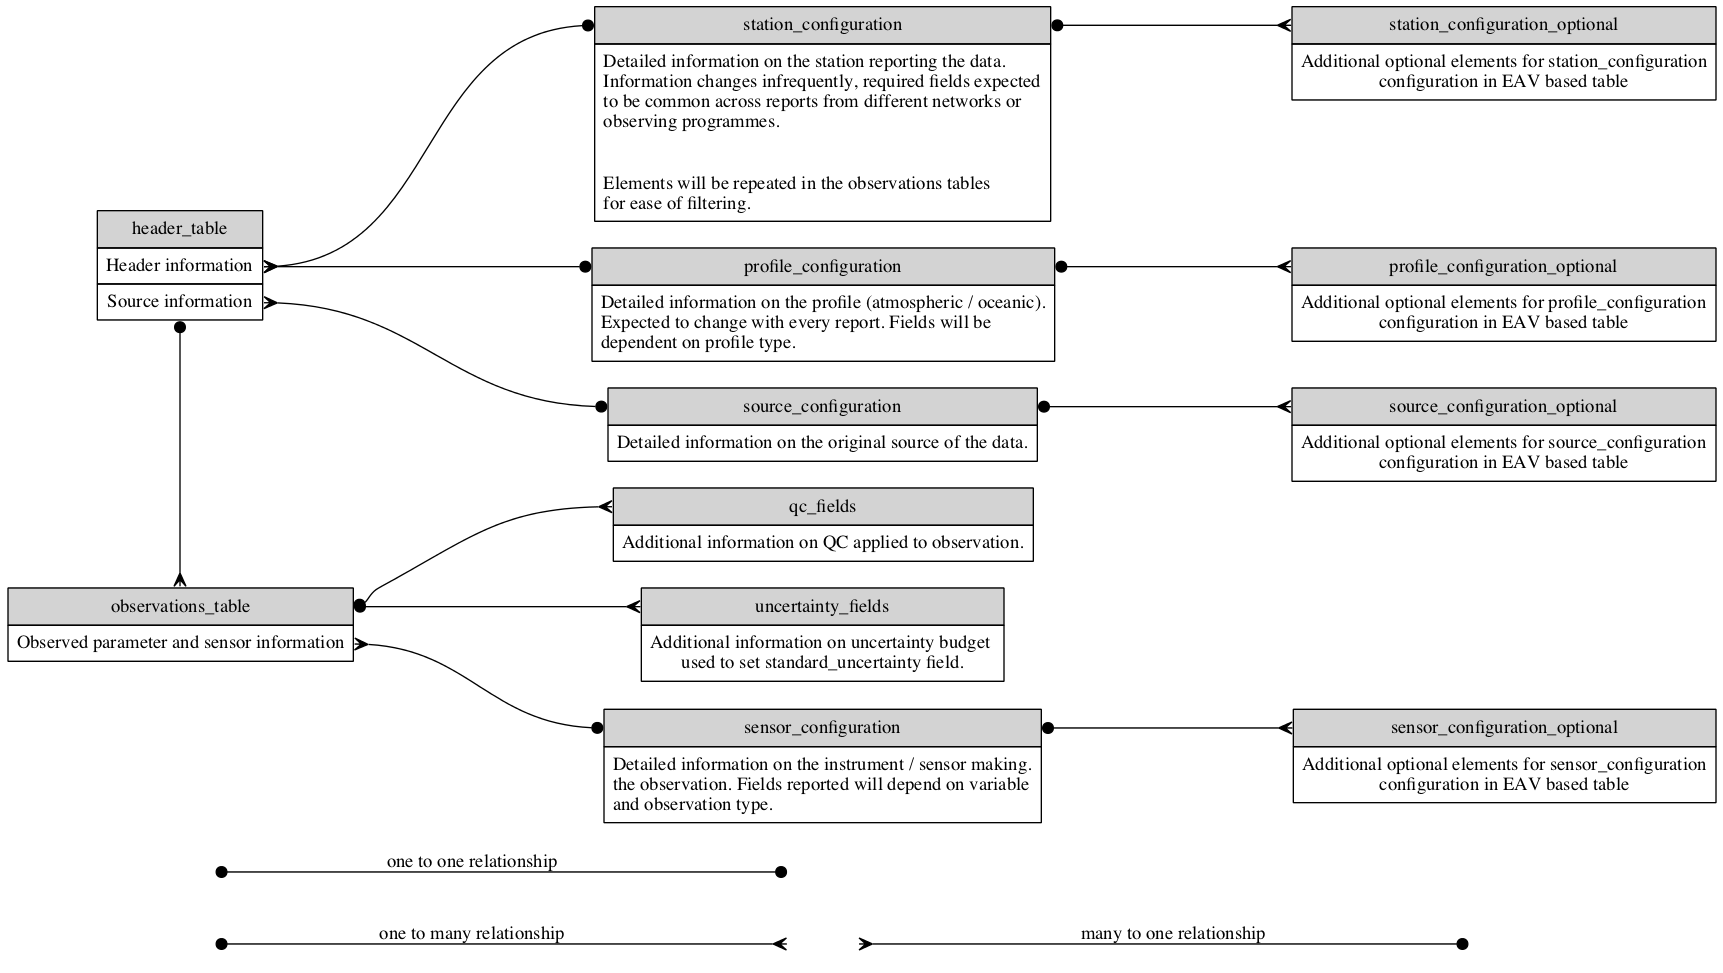
\includegraphics[width=1\textwidth]{/Users/dyb/GitHub/common_data_model/png/cdm_schematic_simple.png}
\caption {Simplified schematic showing overview of common data model}
\end{figure}
\end{landscape}

\begin{landscape}
\subsection{Header table}
\pgfplotstabletypeset[
    empty header,
    begin table=\begin{longtable},
    %every head row/.style={output empty row},
    every nth row={1}{before row=\hline},
    every first row/.append style={
        before row={%
            % Initial caption
            \caption{header\_table (NA)}
            \label{tab:DataTableHeadertable}\\
            % Initial column headers
            \hline\hline             \multicolumn{1} { V{1.125000 in}} { \textbf{\seqsplit{element\_name}}} & 
            \multicolumn{1} { V{1.125000 in}} { \textbf{\seqsplit{occurrence}}} & 
            \multicolumn{1} { V{1.125000 in}} { \textbf{\seqsplit{kind}}} & 
            \multicolumn{1} { V{1.125000 in}} { \textbf{\seqsplit{external\_table}}} & 
            \multicolumn{1} { V{4.000000 in} } {\textbf{\seqsplit{description}}} \\ \hline\hline \endfirsthead
            \multicolumn{5}{c}{Table \thetable\ header\_table (cont.)} \\
            % column headers on additional pages
            \hline\hline             \multicolumn{1} {V{1.125000 in} } { \textbf{\seqsplit{element\_name}}} & 
            \multicolumn{1} {V{1.125000 in} } { \textbf{\seqsplit{occurrence}}} & 
            \multicolumn{1} {V{1.125000 in} } { \textbf{\seqsplit{kind}}} & 
            \multicolumn{1} {V{1.125000 in} } { \textbf{\seqsplit{external\_table}}} & 
            \multicolumn{1} { V{4.000000 in} } {\textbf{\seqsplit{description}}} \\ \hline\hline \endhead
            % Footer on 1st to penultimate pages
            \multicolumn{5}{r}{{Continued on next page}} \\
            \endfoot
            % Footer on last page of table
            \hline
            \multicolumn{5}{r}{{End of table}} \\ 
            \endlastfoot
        }
    },
    %
    end table=\end{longtable},
    col sep=tab,
    string type,
    columns/element_name/.style={
            string type, 
            column type= n{1.125000 in}, 
            string replace*={_}{\_}
        },
    columns/occurrence/.style={
            string type, 
            column type= V{1.125000 in}, 
            string replace*={_}{\_}
        },
    columns/kind/.style={
            string type, 
            column type= V{1.125000 in}, 
            string replace*={_}{\_}
        },
    columns/external_table/.style={
            string type, 
            column type= n{1.125000 in}, 
            string replace*={_}{\_}
        },
    columns/description/.style={
            string type, 
            string replace*={_}{\_},
            column type = V{4.000000 in}
        }
    ]{/Users/dyb/GitHub/C3S_311a_CDM/tables/header_table.csv}

\end{landscape}


%\begin{landscape}
\subsection{Observations table}
\pgfplotstabletypeset[
    empty header,
    begin table=\begin{longtable},
    %every head row/.style={output empty row},
    every nth row={1}{before row=\hline},
    every first row/.append style={
        before row={%
            % Initial caption
            \caption{observations\_table}
            \label{tab:DataTableObservationstable}\\
            % Initial column headers
            \hline\hline             \multicolumn{1} { V{0.933333 in}} { \textbf{\seqsplit{element\_name}}} & 
            \multicolumn{1} { V{0.933333 in}} { \textbf{\seqsplit{kind}}} & 
            \multicolumn{1} { V{0.933333 in}} { \textbf{\seqsplit{external\_table}}} & 
            \multicolumn{1} { V{4.000000 in} } {\textbf{\seqsplit{description}}} \\ \hline\hline \endfirsthead
            \multicolumn{4}{c}{Table \thetable\ observations\_table (cont.)} \\
            % column headers on additional pages
            \hline\hline             \multicolumn{1} {V{0.933333 in} } { \textbf{\seqsplit{element\_name}}} & 
            \multicolumn{1} {V{0.933333 in} } { \textbf{\seqsplit{kind}}} & 
            \multicolumn{1} {V{0.933333 in} } { \textbf{\seqsplit{external\_table}}} & 
            \multicolumn{1} { V{4.000000 in} } {\textbf{\seqsplit{description}}} \\ \hline\hline \endhead
            % Footer on 1st to penultimate pages
            \multicolumn{4}{r}{{Continued on next page}} \\
            \endfoot
            % Footer on last page of table
            \hline
            \multicolumn{4}{r}{{End of table}} \\ 
            \endlastfoot
        }
    },
    %
    end table=\end{longtable},
    col sep=tab,
    string type,
    columns/element_name/.style={
            string type, 
            column type= n{0.933333 in}, 
            string replace*={_}{\_}
        },
    columns/kind/.style={
            string type, 
            column type= V{0.933333 in}, 
            string replace*={_}{\_}
        },
    columns/external_table/.style={
            string type, 
            column type= n{0.933333 in}, 
            string replace*={_}{\_}
        },
    columns/description/.style={
            string type, 
            string replace*={_}{\_},
            column type = V{4.000000 in}
        }
    ]{../table_definitions/observations_table.csv}

%\end{landscape}


\begin{landscape}
\subsection{Station configuration}
\pgfplotstabletypeset[
    empty header,
    begin table=\begin{longtable},
    %every head row/.style={output empty row},
    every nth row={1}{before row=\hline},
    every first row/.append style={
        before row={%
            % Initial caption
            \caption{station\_configuration definition}
            \label{tab:DataTableDefStationconfiguration}\\
            % Initial column headers
            \hline\hline             \multicolumn{1} { V{1.750000 in}} { \textbf{\seqsplit{element\_name}}} & 
            \multicolumn{1} { V{0.800000 in}} { \textbf{\seqsplit{type}}} & 
            \multicolumn{1} { V{1.750000 in}} { \textbf{\seqsplit{external\_table}}} & 
            \multicolumn{1} { V{2.000000 in} } {\textbf{\seqsplit{description}}} \\ \hline\hline \endfirsthead
            \multicolumn{4}{c}{Table \thetable\ station\_configuration (cont.)} \\
            % column headers on additional pages
            \hline\hline             \multicolumn{1} {V{1.750000 in} } { \textbf{\seqsplit{element\_name}}} & 
            \multicolumn{1} {V{0.800000 in} } { \textbf{\seqsplit{type}}} & 
            \multicolumn{1} {V{1.750000 in} } { \textbf{\seqsplit{external\_table}}} & 
            \multicolumn{1} { V{2.000000 in} } {\textbf{\seqsplit{description}}} \\ \hline\hline \endhead
            % Footer on 1st to penultimate pages
            \multicolumn{4}{r}{{Continued on next page}} \\
            \endfoot
            % Footer on last page of table
            \hline
            \multicolumn{4}{r}{{End of table}} \\ 
            \endlastfoot
        }
    },
    %
    end table=\end{longtable},
    col sep=tab,
    string type,
    columns/element_name/.style={
            string type, 
            column type= n{1.750000 in}, 
            string replace*={_}{\_}
        },
    columns/type/.style={
            string type, 
            column type= V{0.800000 in}, 
            string replace*={_}{\_}
        },
    columns/external_table/.style={
            string type, 
            column type= n{1.750000 in}, 
            string replace*={_}{\_}
        },
    columns/description/.style={
            string type, 
            string replace*={_}{\_},
            column type = V{2.000000 in}
        }
    ]{../table_definitions/station_configuration.csv}

\end{landscape}

\pgfplotstabletypeset[
    empty header,
    begin table=\begin{longtable},
    %every head row/.style={output empty row},
    every nth row={1}{before row=\hline},
    every first row/.append style={
        before row={%
            % Initial caption
            \caption{station\_configuration\_optional}
            \label{tab:DataTableStationconfigurationoptional}\\
            % Initial column headers
            \hline\hline             \multicolumn{1} { V{0.933333 in}} { \textbf{\seqsplit{element\_name}}} & 
            \multicolumn{1} { V{0.933333 in}} { \textbf{\seqsplit{kind}}} & 
            \multicolumn{1} { V{0.933333 in}} { \textbf{\seqsplit{external\_table}}} & 
            \multicolumn{1} { V{4.000000 in} } {\textbf{\seqsplit{description}}} \\ \hline\hline \endfirsthead
            \multicolumn{4}{c}{Table \thetable\ station\_configuration\_optional (cont.)} \\
            % column headers on additional pages
            \hline\hline             \multicolumn{1} {V{0.933333 in} } { \textbf{\seqsplit{element\_name}}} & 
            \multicolumn{1} {V{0.933333 in} } { \textbf{\seqsplit{kind}}} & 
            \multicolumn{1} {V{0.933333 in} } { \textbf{\seqsplit{external\_table}}} & 
            \multicolumn{1} { V{4.000000 in} } {\textbf{\seqsplit{description}}} \\ \hline\hline \endhead
            % Footer on 1st to penultimate pages
            \multicolumn{4}{r}{{Continued on next page}} \\
            \endfoot
            % Footer on last page of table
            \hline
            \multicolumn{4}{r}{{End of table}} \\ 
            \endlastfoot
        }
    },
    %
    end table=\end{longtable},
    col sep=tab,
    string type,
    columns/element_name/.style={
            string type, 
            column type= n{0.933333 in}, 
            string replace*={_}{\_}
        },
    columns/kind/.style={
            string type, 
            column type= V{0.933333 in}, 
            string replace*={_}{\_}
        },
    columns/external_table/.style={
            string type, 
            column type= n{0.933333 in}, 
            string replace*={_}{\_}
        },
    columns/description/.style={
            string type, 
            string replace*={_}{\_},
            column type = V{4.000000 in}
        }
    ]{../table_definitions/station_configuration_optional.csv}


\begin{landscape}
\subsection{Profile configuration}
\pgfplotstabletypeset[
    empty header,
    begin table=\begin{longtable},
    %every head row/.style={output empty row},
    every nth row={1}{before row=\hline},
    every first row/.append style={
        before row={%
            % Initial caption
            \caption{profile\_configuration definition}
            \label{tab:DataTableDefProfileconfiguration}\\
            % Initial column headers
            \hline\hline             \multicolumn{1} { V{1.750000 in}} { \textbf{\seqsplit{element\_name}}} & 
            \multicolumn{1} { V{0.800000 in}} { \textbf{\seqsplit{kind}}} & 
            \multicolumn{1} { V{1.750000 in}} { \textbf{\seqsplit{external\_table}}} & 
            \multicolumn{1} { V{2.000000 in} } {\textbf{\seqsplit{description}}} \\ \hline\hline \endfirsthead
            \multicolumn{4}{c}{Table \thetable\ profile\_configuration (cont.)} \\
            % column headers on additional pages
            \hline\hline             \multicolumn{1} {V{1.750000 in} } { \textbf{\seqsplit{element\_name}}} & 
            \multicolumn{1} {V{0.800000 in} } { \textbf{\seqsplit{kind}}} & 
            \multicolumn{1} {V{1.750000 in} } { \textbf{\seqsplit{external\_table}}} & 
            \multicolumn{1} { V{2.000000 in} } {\textbf{\seqsplit{description}}} \\ \hline\hline \endhead
            % Footer on 1st to penultimate pages
            \multicolumn{4}{r}{{Continued on next page}} \\
            \endfoot
            % Footer on last page of table
            \hline
            \multicolumn{4}{r}{{End of table}} \\ 
            \endlastfoot
        }
    },
    %
    end table=\end{longtable},
    col sep=tab,
    string type,
    columns/element_name/.style={
            string type, 
            column type= n{1.750000 in}, 
            string replace*={_}{\_}
        },
    columns/kind/.style={
            string type, 
            column type= V{0.800000 in}, 
            string replace*={_}{\_}
        },
    columns/external_table/.style={
            string type, 
            column type= n{1.750000 in}, 
            string replace*={_}{\_}
        },
    columns/description/.style={
            string type, 
            string replace*={_}{\_},
            column type = V{2.000000 in}
        }
    ]{../table_definitions/profile_configuration.csv}

\end{landscape}

\pgfplotstabletypeset[
    empty header,
    begin table=\begin{longtable},
    %every head row/.style={output empty row},
    every nth row={1}{before row=\hline},
    every first row/.append style={
        before row={%
            % Initial caption
            \caption{profile\_configuration\_optional}
            \label{tab:DataTableProfileconfigurationoptional}\\
            % Initial column headers
            \hline\hline             \multicolumn{1} { V{0.933333 in}} { \textbf{\seqsplit{element\_name}}} & 
            \multicolumn{1} { V{0.933333 in}} { \textbf{\seqsplit{kind}}} & 
            \multicolumn{1} { V{0.933333 in}} { \textbf{\seqsplit{external\_table}}} & 
            \multicolumn{1} { V{4.000000 in} } {\textbf{\seqsplit{description}}} \\ \hline\hline \endfirsthead
            \multicolumn{4}{c}{Table \thetable\ profile\_configuration\_optional (cont.)} \\
            % column headers on additional pages
            \hline\hline             \multicolumn{1} {V{0.933333 in} } { \textbf{\seqsplit{element\_name}}} & 
            \multicolumn{1} {V{0.933333 in} } { \textbf{\seqsplit{kind}}} & 
            \multicolumn{1} {V{0.933333 in} } { \textbf{\seqsplit{external\_table}}} & 
            \multicolumn{1} { V{4.000000 in} } {\textbf{\seqsplit{description}}} \\ \hline\hline \endhead
            % Footer on 1st to penultimate pages
            \multicolumn{4}{r}{{Continued on next page}} \\
            \endfoot
            % Footer on last page of table
            \hline
            \multicolumn{4}{r}{{End of table}} \\ 
            \endlastfoot
        }
    },
    %
    end table=\end{longtable},
    col sep=tab,
    string type,
    columns/element_name/.style={
            string type, 
            column type= n{0.933333 in}, 
            string replace*={_}{\_}
        },
    columns/kind/.style={
            string type, 
            column type= V{0.933333 in}, 
            string replace*={_}{\_}
        },
    columns/external_table/.style={
            string type, 
            column type= n{0.933333 in}, 
            string replace*={_}{\_}
        },
    columns/description/.style={
            string type, 
            string replace*={_}{\_},
            column type = V{4.000000 in}
        }
    ]{../table_definitions/profile_configuration_optional.csv}



\begin{landscape}
\subsection{Source configuration}
\pgfplotstabletypeset[
    empty header,
    begin table=\begin{longtable},
    %every head row/.style={output empty row},
    every nth row={1}{before row=\hline},
    every first row/.append style={
        before row={%
            % Initial caption
            \caption{source\_configuration definition}
            \label{tab:DataTableDefSourceconfiguration}\\
            % Initial column headers
            \hline\hline             \multicolumn{1} { V{1.750000 in}} { \textbf{\seqsplit{element\_name}}} & 
            \multicolumn{1} { V{0.800000 in}} { \textbf{\seqsplit{type}}} & 
            \multicolumn{1} { V{1.750000 in}} { \textbf{\seqsplit{external\_table}}} & 
            \multicolumn{1} { V{2.000000 in} } {\textbf{\seqsplit{description}}} \\ \hline\hline \endfirsthead
            \multicolumn{4}{c}{Table \thetable\ source\_configuration (cont.)} \\
            % column headers on additional pages
            \hline\hline             \multicolumn{1} {V{1.750000 in} } { \textbf{\seqsplit{element\_name}}} & 
            \multicolumn{1} {V{0.800000 in} } { \textbf{\seqsplit{type}}} & 
            \multicolumn{1} {V{1.750000 in} } { \textbf{\seqsplit{external\_table}}} & 
            \multicolumn{1} { V{2.000000 in} } {\textbf{\seqsplit{description}}} \\ \hline\hline \endhead
            % Footer on 1st to penultimate pages
            \multicolumn{4}{r}{{Continued on next page}} \\
            \endfoot
            % Footer on last page of table
            \hline
            \multicolumn{4}{r}{{End of table}} \\ 
            \endlastfoot
        }
    },
    %
    end table=\end{longtable},
    col sep=tab,
    string type,
    columns/element_name/.style={
            string type, 
            column type= n{1.750000 in}, 
            string replace*={_}{\_}
        },
    columns/type/.style={
            string type, 
            column type= V{0.800000 in}, 
            string replace*={_}{\_}
        },
    columns/external_table/.style={
            string type, 
            column type= n{1.750000 in}, 
            string replace*={_}{\_}
        },
    columns/description/.style={
            string type, 
            string replace*={_}{\_},
            column type = V{2.000000 in}
        }
    ]{../table_definitions/source_configuration.csv}

\end{landscape}

\pgfplotstabletypeset[
    empty header,
    begin table=\begin{longtable},
    %every head row/.style={output empty row},
    every nth row={1}{before row=\hline},
    every first row/.append style={
        before row={%
            % Initial caption
            \caption{source\_configuration\_optional definition}
            \label{tab:DataTableDefSourceconfigurationoptional}\\
            % Initial column headers
            \hline\hline             \multicolumn{1} { V{1.750000 in}} { \textbf{\seqsplit{element\_name}}} & 
            \multicolumn{1} { V{0.800000 in}} { \textbf{\seqsplit{kind}}} & 
            \multicolumn{1} { V{1.750000 in}} { \textbf{\seqsplit{external\_table}}} & 
            \multicolumn{1} { V{2.000000 in} } {\textbf{\seqsplit{description}}} \\ \hline\hline \endfirsthead
            \multicolumn{4}{c}{Table \thetable\ source\_configuration\_optional (cont.)} \\
            % column headers on additional pages
            \hline\hline             \multicolumn{1} {V{1.750000 in} } { \textbf{\seqsplit{element\_name}}} & 
            \multicolumn{1} {V{0.800000 in} } { \textbf{\seqsplit{kind}}} & 
            \multicolumn{1} {V{1.750000 in} } { \textbf{\seqsplit{external\_table}}} & 
            \multicolumn{1} { V{2.000000 in} } {\textbf{\seqsplit{description}}} \\ \hline\hline \endhead
            % Footer on 1st to penultimate pages
            \multicolumn{4}{r}{{Continued on next page}} \\
            \endfoot
            % Footer on last page of table
            \hline
            \multicolumn{4}{r}{{End of table}} \\ 
            \endlastfoot
        }
    },
    %
    end table=\end{longtable},
    col sep=tab,
    string type,
    columns/element_name/.style={
            string type, 
            column type= n{1.750000 in}, 
            string replace*={_}{\_}
        },
    columns/kind/.style={
            string type, 
            column type= V{0.800000 in}, 
            string replace*={_}{\_}
        },
    columns/external_table/.style={
            string type, 
            column type= n{1.750000 in}, 
            string replace*={_}{\_}
        },
    columns/description/.style={
            string type, 
            string replace*={_}{\_},
            column type = V{2.000000 in}
        }
    ]{../table_definitions/source_configuration_optional.csv}


\begin{landscape}
\subsection{Sensor configuration}
\pgfplotstabletypeset[
    empty header,
    begin table=\begin{longtable},
    %every head row/.style={output empty row},
    every nth row={1}{before row=\hline},
    every first row/.append style={
        before row={%
            % Initial caption
            \caption{sensor\_configuration}
            \label{tab:DataTableSensorconfiguration}\\
            % Initial column headers
            \hline\hline             \multicolumn{1} { V{1.475000 in}} { \textbf{\seqsplit{element\_name}}} & 
            \multicolumn{1} { V{1.475000 in}} { \textbf{\seqsplit{occurrence}}} & 
            \multicolumn{1} { V{1.475000 in}} { \textbf{\seqsplit{type}}} & 
            \multicolumn{1} { V{1.475000 in}} { \textbf{\seqsplit{external\_table}}} & 
            \multicolumn{1} { V{3.000000 in} } {\textbf{\seqsplit{description}}} \\ \hline\hline \endfirsthead
            \multicolumn{5}{c}{Table \thetable\ sensor\_configuration (cont.)} \\
            % column headers on additional pages
            \hline\hline             \multicolumn{1} {V{1.475000 in} } { \textbf{\seqsplit{element\_name}}} & 
            \multicolumn{1} {V{1.475000 in} } { \textbf{\seqsplit{occurrence}}} & 
            \multicolumn{1} {V{1.475000 in} } { \textbf{\seqsplit{type}}} & 
            \multicolumn{1} {V{1.475000 in} } { \textbf{\seqsplit{external\_table}}} & 
            \multicolumn{1} { V{3.000000 in} } {\textbf{\seqsplit{description}}} \\ \hline\hline \endhead
            % Footer on 1st to penultimate pages
            \multicolumn{5}{r}{{Continued on next page}} \\
            \endfoot
            % Footer on last page of table
            \hline
            \multicolumn{5}{r}{{End of table}} \\ 
            \endlastfoot
        }
    },
    %
    end table=\end{longtable},
    col sep=tab,
    string type,
    columns/element_name/.style={
            string type, 
            column type= n{1.475000 in}, 
            string replace*={_}{\_}
        },
    columns/occurrence/.style={
            string type, 
            column type= V{1.475000 in}, 
            string replace*={_}{\_}
        },
    columns/type/.style={
            string type, 
            column type= V{1.475000 in}, 
            string replace*={_}{\_}
        },
    columns/external_table/.style={
            string type, 
            column type= n{1.475000 in}, 
            string replace*={_}{\_}
        },
    columns/description/.style={
            string type, 
            string replace*={_}{\_},
            column type = V{3.000000 in}
        }
    ]{/Users/dyb/GitHub/C3S_311a_CDM/tables/sensor_configuration.csv}

\end{landscape}

\pgfplotstabletypeset[
    empty header,
    begin table=\begin{longtable},
    %every head row/.style={output empty row},
    every nth row={1}{before row=\hline},
    every first row/.append style={
        before row={%
            % Initial caption
            \caption{sensor\_configuration\_optional definition}
            \label{tab:DataTableDefSensorconfigurationoptional}\\
            % Initial column headers
            \hline\hline             \multicolumn{1} { V{1.750000 in}} { \textbf{\seqsplit{element\_name}}} & 
            \multicolumn{1} { V{0.800000 in}} { \textbf{\seqsplit{kind}}} & 
            \multicolumn{1} { V{1.750000 in}} { \textbf{\seqsplit{external\_table}}} & 
            \multicolumn{1} { V{2.000000 in} } {\textbf{\seqsplit{description}}} \\ \hline\hline \endfirsthead
            \multicolumn{4}{c}{Table \thetable\ sensor\_configuration\_optional (cont.)} \\
            % column headers on additional pages
            \hline\hline             \multicolumn{1} {V{1.750000 in} } { \textbf{\seqsplit{element\_name}}} & 
            \multicolumn{1} {V{0.800000 in} } { \textbf{\seqsplit{kind}}} & 
            \multicolumn{1} {V{1.750000 in} } { \textbf{\seqsplit{external\_table}}} & 
            \multicolumn{1} { V{2.000000 in} } {\textbf{\seqsplit{description}}} \\ \hline\hline \endhead
            % Footer on 1st to penultimate pages
            \multicolumn{4}{r}{{Continued on next page}} \\
            \endfoot
            % Footer on last page of table
            \hline
            \multicolumn{4}{r}{{End of table}} \\ 
            \endlastfoot
        }
    },
    %
    end table=\end{longtable},
    col sep=tab,
    string type,
    columns/element_name/.style={
            string type, 
            column type= n{1.750000 in}, 
            string replace*={_}{\_}
        },
    columns/kind/.style={
            string type, 
            column type= V{0.800000 in}, 
            string replace*={_}{\_}
        },
    columns/external_table/.style={
            string type, 
            column type= n{1.750000 in}, 
            string replace*={_}{\_}
        },
    columns/description/.style={
            string type, 
            string replace*={_}{\_},
            column type = V{2.000000 in}
        }
    ]{../table_definitions/sensor_configuration_optional.csv}



\subsection {Quality control flags}
A single QC flag is provided in the observations table for the observed value. Additional flags can be provided using the qc\_table and by setting the advanced\_qc flag to true in the observations\_table.\\
\pgfplotstabletypeset[
    empty header,
    begin table=\begin{longtable},
    %every head row/.style={output empty row},
    every nth row={1}{before row=\hline},
    every first row/.append style={
        before row={%
            % Initial caption
            \caption{qc\_table}
            \label{tab:DataTableQctable}\\
            % Initial column headers
            \hline\hline             \multicolumn{1} { V{0.933333 in}} { \textbf{\seqsplit{element\_name}}} & 
            \multicolumn{1} { V{0.933333 in}} { \textbf{\seqsplit{kind}}} & 
            \multicolumn{1} { V{0.933333 in}} { \textbf{\seqsplit{external\_table}}} & 
            \multicolumn{1} { V{4.000000 in} } {\textbf{\seqsplit{description}}} \\ \hline\hline \endfirsthead
            \multicolumn{4}{c}{Table \thetable\ qc\_table (cont.)} \\
            % column headers on additional pages
            \hline\hline             \multicolumn{1} {V{0.933333 in} } { \textbf{\seqsplit{element\_name}}} & 
            \multicolumn{1} {V{0.933333 in} } { \textbf{\seqsplit{kind}}} & 
            \multicolumn{1} {V{0.933333 in} } { \textbf{\seqsplit{external\_table}}} & 
            \multicolumn{1} { V{4.000000 in} } {\textbf{\seqsplit{description}}} \\ \hline\hline \endhead
            % Footer on 1st to penultimate pages
            \multicolumn{4}{r}{{Continued on next page}} \\
            \endfoot
            % Footer on last page of table
            \hline
            \multicolumn{4}{r}{{End of table}} \\ 
            \endlastfoot
        }
    },
    %
    end table=\end{longtable},
    col sep=tab,
    string type,
    columns/element_name/.style={
            string type, 
            column type= n{0.933333 in}, 
            string replace*={_}{\_}
        },
    columns/kind/.style={
            string type, 
            column type= V{0.933333 in}, 
            string replace*={_}{\_}
        },
    columns/external_table/.style={
            string type, 
            column type= n{0.933333 in}, 
            string replace*={_}{\_}
        },
    columns/description/.style={
            string type, 
            string replace*={_}{\_},
            column type = V{4.000000 in}
        }
    ]{../table_definitions/qc_table.csv}


\subsection {Uncertainty budget}
A single standard uncertainty value is provided for each observed value in the observations table. Additional values can be provided using the uncertainty\_table and by setting the advanced\_uncertainty to true in the observations\_table.\\
\pgfplotstabletypeset[
    empty header,
    begin table=\begin{longtable},
    %every head row/.style={output empty row},
    every nth row={1}{before row=\hline},
    every first row/.append style={
        before row={%
            % Initial caption
            \caption{uncertainty\_table}
            \label{tab:DataTableUncertaintytable}\\
            % Initial column headers
            \hline\hline             \multicolumn{1} { V{0.933333 in}} { \textbf{\seqsplit{element\_name}}} & 
            \multicolumn{1} { V{0.933333 in}} { \textbf{\seqsplit{kind}}} & 
            \multicolumn{1} { V{0.933333 in}} { \textbf{\seqsplit{external\_table}}} & 
            \multicolumn{1} { V{4.000000 in} } {\textbf{\seqsplit{description}}} \\ \hline\hline \endfirsthead
            \multicolumn{4}{c}{Table \thetable\ uncertainty\_table (cont.)} \\
            % column headers on additional pages
            \hline\hline             \multicolumn{1} {V{0.933333 in} } { \textbf{\seqsplit{element\_name}}} & 
            \multicolumn{1} {V{0.933333 in} } { \textbf{\seqsplit{kind}}} & 
            \multicolumn{1} {V{0.933333 in} } { \textbf{\seqsplit{external\_table}}} & 
            \multicolumn{1} { V{4.000000 in} } {\textbf{\seqsplit{description}}} \\ \hline\hline \endhead
            % Footer on 1st to penultimate pages
            \multicolumn{4}{r}{{Continued on next page}} \\
            \endfoot
            % Footer on last page of table
            \hline
            \multicolumn{4}{r}{{End of table}} \\ 
            \endlastfoot
        }
    },
    %
    end table=\end{longtable},
    col sep=tab,
    string type,
    columns/element_name/.style={
            string type, 
            column type= n{0.933333 in}, 
            string replace*={_}{\_}
        },
    columns/kind/.style={
            string type, 
            column type= V{0.933333 in}, 
            string replace*={_}{\_}
        },
    columns/external_table/.style={
            string type, 
            column type= n{0.933333 in}, 
            string replace*={_}{\_}
        },
    columns/description/.style={
            string type, 
            string replace*={_}{\_},
            column type = V{4.000000 in}
        }
    ]{../table_definitions/uncertainty_table.csv}


\subsection {Homogenisation data}
\pgfplotstabletypeset[
    empty header,
    begin table=\begin{longtable},
    %every head row/.style={output empty row},
    every nth row={1}{before row=\hline},
    every first row/.append style={
        before row={%
            % Initial caption
            \caption{homogenisation\_table definition}
            \label{tab:DataTableDefHomogenisationtable}\\
            % Initial column headers
            \hline\hline             \multicolumn{1} { V{1.750000 in}} { \textbf{\seqsplit{element\_name}}} & 
            \multicolumn{1} { V{0.800000 in}} { \textbf{\seqsplit{kind}}} & 
            \multicolumn{1} { V{1.750000 in}} { \textbf{\seqsplit{external\_table}}} & 
            \multicolumn{1} { V{2.000000 in} } {\textbf{\seqsplit{description}}} \\ \hline\hline \endfirsthead
            \multicolumn{4}{c}{Table \thetable\ homogenisation\_table (cont.)} \\
            % column headers on additional pages
            \hline\hline             \multicolumn{1} {V{1.750000 in} } { \textbf{\seqsplit{element\_name}}} & 
            \multicolumn{1} {V{0.800000 in} } { \textbf{\seqsplit{kind}}} & 
            \multicolumn{1} {V{1.750000 in} } { \textbf{\seqsplit{external\_table}}} & 
            \multicolumn{1} { V{2.000000 in} } {\textbf{\seqsplit{description}}} \\ \hline\hline \endhead
            % Footer on 1st to penultimate pages
            \multicolumn{4}{r}{{Continued on next page}} \\
            \endfoot
            % Footer on last page of table
            \hline
            \multicolumn{4}{r}{{End of table}} \\ 
            \endlastfoot
        }
    },
    %
    end table=\end{longtable},
    col sep=tab,
    string type,
    columns/element_name/.style={
            string type, 
            column type= n{1.750000 in}, 
            string replace*={_}{\_}
        },
    columns/kind/.style={
            string type, 
            column type= V{0.800000 in}, 
            string replace*={_}{\_}
        },
    columns/external_table/.style={
            string type, 
            column type= n{1.750000 in}, 
            string replace*={_}{\_}
        },
    columns/description/.style={
            string type, 
            string replace*={_}{\_},
            column type = V{2.000000 in}
        }
    ]{../table_definitions/homogenisation_table.csv}


\section {References}

\hangindent=2em\hangafter=1 Freeman E., S. D. Woodruff, S. J. Worley, S. J. Lubker, E. C. Kent, W. E. Angel, D. I. Berry , P. Brohan, R. Eastman, L. Gates, W. Gloeden, Z. Ji, J. Lawrimore, N. A. Rayner, G. Rosenhagen, S. R. Smith, 2017: ICOADS Release 3.0: A Major Update to the Historical Marine Climate Record, International Journal of Climatology, 37, 2211 - 2232. doi:10.1002/joc.4775\\

\hangindent=2em\hangafter=1 GCOS, 2016: The Global Observing System for Climate: Implementation Needs. GCOS-200 / GOOS-214, WMO, Geneva, 342pp.\\

\hangindent=2em\hangafter=1 Hersbach, H., P. Poli and D. Dee, 2015: The observation feedback archive for ICOADS and ISPD datasets. ERA Report Series No. 18, ECMWF, Reading, UK, \\31pp.

\hangindent=2em\hangafter=1 Saarinen, S., 2004: ODB User guide (draft 1st edition), ECMWF, Reading, UK, 289pp.\\

\hangindent=2em\hangafter=1 WMO, 2015a: Manual On Codes (WMO-No 306), Volume I.2, Part B - Binary Codes, WMO, Geneva.\\

\hangindent=2em\hangafter=1 WMO, 2015b:  Manual on the WMO Integrated Global Observing System: Annex VIII to the Technical Regulations (WMO-No 1160), WMO, Geneva.\\
\newpage
\section {Appendix}
\subsection {Table definitions}

\subsubsection {Data tables}
\pgfplotstabletypeset[
    empty header,
    begin table=\begin{longtable},
    %every head row/.style={output empty row},
    every nth row={1}{before row=\hline},
    every first row/.append style={
        before row={%
            % Initial caption
            \caption{adjustment}
            \label{tab:DataTableAdjustment}\\
            % Initial column headers
            \hline\hline             \multicolumn{1} { V{0.933333 in}} { \textbf{\seqsplit{element\_name}}} & 
            \multicolumn{1} { V{0.933333 in}} { \textbf{\seqsplit{kind}}} & 
            \multicolumn{1} { V{0.933333 in}} { \textbf{\seqsplit{external\_table}}} & 
            \multicolumn{1} { V{4.000000 in} } {\textbf{\seqsplit{description}}} \\ \hline\hline \endfirsthead
            \multicolumn{4}{c}{Table \thetable\ adjustment (cont.)} \\
            % column headers on additional pages
            \hline\hline             \multicolumn{1} {V{0.933333 in} } { \textbf{\seqsplit{element\_name}}} & 
            \multicolumn{1} {V{0.933333 in} } { \textbf{\seqsplit{kind}}} & 
            \multicolumn{1} {V{0.933333 in} } { \textbf{\seqsplit{external\_table}}} & 
            \multicolumn{1} { V{4.000000 in} } {\textbf{\seqsplit{description}}} \\ \hline\hline \endhead
            % Footer on 1st to penultimate pages
            \multicolumn{4}{r}{{Continued on next page}} \\
            \endfoot
            % Footer on last page of table
            \hline
            \multicolumn{4}{r}{{End of table}} \\ 
            \endlastfoot
        }
    },
    %
    end table=\end{longtable},
    col sep=tab,
    string type,
    columns/element_name/.style={
            string type, 
            column type= n{0.933333 in}, 
            string replace*={_}{\_}
        },
    columns/kind/.style={
            string type, 
            column type= V{0.933333 in}, 
            string replace*={_}{\_}
        },
    columns/external_table/.style={
            string type, 
            column type= n{0.933333 in}, 
            string replace*={_}{\_}
        },
    columns/description/.style={
            string type, 
            string replace*={_}{\_},
            column type = V{4.000000 in}
        }
    ]{../table_definitions/adjustment.csv}
 % data table
\pgfplotstabletypeset[
    empty header,
    begin table=\begin{longtable},
    %every head row/.style={output empty row},
    every nth row={1}{before row=\hline},
    every first row/.append style={
        before row={%
            % Initial caption
            \caption{contact}
            \label{tab:DataTableContact}\\
            % Initial column headers
            \hline\hline             \multicolumn{1} { V{0.933333 in}} { \textbf{\seqsplit{element\_name}}} & 
            \multicolumn{1} { V{0.933333 in}} { \textbf{\seqsplit{kind}}} & 
            \multicolumn{1} { V{0.933333 in}} { \textbf{\seqsplit{external\_table}}} & 
            \multicolumn{1} { V{4.000000 in} } {\textbf{\seqsplit{description}}} \\ \hline\hline \endfirsthead
            \multicolumn{4}{c}{Table \thetable\ contact (cont.)} \\
            % column headers on additional pages
            \hline\hline             \multicolumn{1} {V{0.933333 in} } { \textbf{\seqsplit{element\_name}}} & 
            \multicolumn{1} {V{0.933333 in} } { \textbf{\seqsplit{kind}}} & 
            \multicolumn{1} {V{0.933333 in} } { \textbf{\seqsplit{external\_table}}} & 
            \multicolumn{1} { V{4.000000 in} } {\textbf{\seqsplit{description}}} \\ \hline\hline \endhead
            % Footer on 1st to penultimate pages
            \multicolumn{4}{r}{{Continued on next page}} \\
            \endfoot
            % Footer on last page of table
            \hline
            \multicolumn{4}{r}{{End of table}} \\ 
            \endlastfoot
        }
    },
    %
    end table=\end{longtable},
    col sep=tab,
    string type,
    columns/element_name/.style={
            string type, 
            column type= n{0.933333 in}, 
            string replace*={_}{\_}
        },
    columns/kind/.style={
            string type, 
            column type= V{0.933333 in}, 
            string replace*={_}{\_}
        },
    columns/external_table/.style={
            string type, 
            column type= n{0.933333 in}, 
            string replace*={_}{\_}
        },
    columns/description/.style={
            string type, 
            string replace*={_}{\_},
            column type = V{4.000000 in}
        }
    ]{../table_definitions/contact.csv}
 % data table
\pgfplotstabletypeset[
    empty header,
    begin table=\begin{longtable},
    %every head row/.style={output empty row},
    every nth row={1}{before row=\hline},
    every first row/.append style={
        before row={%
            % Initial caption
            \caption{header\_table}
            \label{tab:DataTableHeadertable}\\
            % Initial column headers
            \hline\hline             \multicolumn{1} { V{0.933333 in}} { \textbf{\seqsplit{element\_name}}} & 
            \multicolumn{1} { V{0.933333 in}} { \textbf{\seqsplit{kind}}} & 
            \multicolumn{1} { V{0.933333 in}} { \textbf{\seqsplit{external\_table}}} & 
            \multicolumn{1} { V{4.000000 in} } {\textbf{\seqsplit{description}}} \\ \hline\hline \endfirsthead
            \multicolumn{4}{c}{Table \thetable\ header\_table (cont.)} \\
            % column headers on additional pages
            \hline\hline             \multicolumn{1} {V{0.933333 in} } { \textbf{\seqsplit{element\_name}}} & 
            \multicolumn{1} {V{0.933333 in} } { \textbf{\seqsplit{kind}}} & 
            \multicolumn{1} {V{0.933333 in} } { \textbf{\seqsplit{external\_table}}} & 
            \multicolumn{1} { V{4.000000 in} } {\textbf{\seqsplit{description}}} \\ \hline\hline \endhead
            % Footer on 1st to penultimate pages
            \multicolumn{4}{r}{{Continued on next page}} \\
            \endfoot
            % Footer on last page of table
            \hline
            \multicolumn{4}{r}{{End of table}} \\ 
            \endlastfoot
        }
    },
    %
    end table=\end{longtable},
    col sep=tab,
    string type,
    columns/element_name/.style={
            string type, 
            column type= n{0.933333 in}, 
            string replace*={_}{\_}
        },
    columns/kind/.style={
            string type, 
            column type= V{0.933333 in}, 
            string replace*={_}{\_}
        },
    columns/external_table/.style={
            string type, 
            column type= n{0.933333 in}, 
            string replace*={_}{\_}
        },
    columns/description/.style={
            string type, 
            string replace*={_}{\_},
            column type = V{4.000000 in}
        }
    ]{../table_definitions/header_table.csv}
 % data table
\pgfplotstabletypeset[
    empty header,
    begin table=\begin{longtable},
    %every head row/.style={output empty row},
    every nth row={1}{before row=\hline},
    every first row/.append style={
        before row={%
            % Initial caption
            \caption{homogenisation\_table definition}
            \label{tab:DataTableDefHomogenisationtable}\\
            % Initial column headers
            \hline\hline             \multicolumn{1} { V{1.750000 in}} { \textbf{\seqsplit{element\_name}}} & 
            \multicolumn{1} { V{0.800000 in}} { \textbf{\seqsplit{kind}}} & 
            \multicolumn{1} { V{1.750000 in}} { \textbf{\seqsplit{external\_table}}} & 
            \multicolumn{1} { V{2.000000 in} } {\textbf{\seqsplit{description}}} \\ \hline\hline \endfirsthead
            \multicolumn{4}{c}{Table \thetable\ homogenisation\_table (cont.)} \\
            % column headers on additional pages
            \hline\hline             \multicolumn{1} {V{1.750000 in} } { \textbf{\seqsplit{element\_name}}} & 
            \multicolumn{1} {V{0.800000 in} } { \textbf{\seqsplit{kind}}} & 
            \multicolumn{1} {V{1.750000 in} } { \textbf{\seqsplit{external\_table}}} & 
            \multicolumn{1} { V{2.000000 in} } {\textbf{\seqsplit{description}}} \\ \hline\hline \endhead
            % Footer on 1st to penultimate pages
            \multicolumn{4}{r}{{Continued on next page}} \\
            \endfoot
            % Footer on last page of table
            \hline
            \multicolumn{4}{r}{{End of table}} \\ 
            \endlastfoot
        }
    },
    %
    end table=\end{longtable},
    col sep=tab,
    string type,
    columns/element_name/.style={
            string type, 
            column type= n{1.750000 in}, 
            string replace*={_}{\_}
        },
    columns/kind/.style={
            string type, 
            column type= V{0.800000 in}, 
            string replace*={_}{\_}
        },
    columns/external_table/.style={
            string type, 
            column type= n{1.750000 in}, 
            string replace*={_}{\_}
        },
    columns/description/.style={
            string type, 
            string replace*={_}{\_},
            column type = V{2.000000 in}
        }
    ]{../table_definitions/homogenisation_table.csv}

\pgfplotstabletypeset[
    empty header,
    begin table=\begin{longtable},
    %every head row/.style={output empty row},
    every nth row={1}{before row=\hline},
    every first row/.append style={
        before row={%
            % Initial caption
            \caption{observations\_table}
            \label{tab:DataTableObservationstable}\\
            % Initial column headers
            \hline\hline             \multicolumn{1} { V{0.933333 in}} { \textbf{\seqsplit{element\_name}}} & 
            \multicolumn{1} { V{0.933333 in}} { \textbf{\seqsplit{kind}}} & 
            \multicolumn{1} { V{0.933333 in}} { \textbf{\seqsplit{external\_table}}} & 
            \multicolumn{1} { V{4.000000 in} } {\textbf{\seqsplit{description}}} \\ \hline\hline \endfirsthead
            \multicolumn{4}{c}{Table \thetable\ observations\_table (cont.)} \\
            % column headers on additional pages
            \hline\hline             \multicolumn{1} {V{0.933333 in} } { \textbf{\seqsplit{element\_name}}} & 
            \multicolumn{1} {V{0.933333 in} } { \textbf{\seqsplit{kind}}} & 
            \multicolumn{1} {V{0.933333 in} } { \textbf{\seqsplit{external\_table}}} & 
            \multicolumn{1} { V{4.000000 in} } {\textbf{\seqsplit{description}}} \\ \hline\hline \endhead
            % Footer on 1st to penultimate pages
            \multicolumn{4}{r}{{Continued on next page}} \\
            \endfoot
            % Footer on last page of table
            \hline
            \multicolumn{4}{r}{{End of table}} \\ 
            \endlastfoot
        }
    },
    %
    end table=\end{longtable},
    col sep=tab,
    string type,
    columns/element_name/.style={
            string type, 
            column type= n{0.933333 in}, 
            string replace*={_}{\_}
        },
    columns/kind/.style={
            string type, 
            column type= V{0.933333 in}, 
            string replace*={_}{\_}
        },
    columns/external_table/.style={
            string type, 
            column type= n{0.933333 in}, 
            string replace*={_}{\_}
        },
    columns/description/.style={
            string type, 
            string replace*={_}{\_},
            column type = V{4.000000 in}
        }
    ]{../table_definitions/observations_table.csv}

\pgfplotstabletypeset[
    empty header,
    begin table=\begin{longtable},
    %every head row/.style={output empty row},
    every nth row={1}{before row=\hline},
    every first row/.append style={
        before row={%
            % Initial caption
            \caption{organisation definition}
            \label{tab:DataTableDefOrganisation}\\
            % Initial column headers
            \hline\hline             \multicolumn{1} { V{1.750000 in}} { \textbf{\seqsplit{element\_name}}} & 
            \multicolumn{1} { V{0.800000 in}} { \textbf{\seqsplit{kind}}} & 
            \multicolumn{1} { V{1.750000 in}} { \textbf{\seqsplit{external\_table}}} & 
            \multicolumn{1} { V{2.000000 in} } {\textbf{\seqsplit{description}}} \\ \hline\hline \endfirsthead
            \multicolumn{4}{c}{Table \thetable\ organisation (cont.)} \\
            % column headers on additional pages
            \hline\hline             \multicolumn{1} {V{1.750000 in} } { \textbf{\seqsplit{element\_name}}} & 
            \multicolumn{1} {V{0.800000 in} } { \textbf{\seqsplit{kind}}} & 
            \multicolumn{1} {V{1.750000 in} } { \textbf{\seqsplit{external\_table}}} & 
            \multicolumn{1} { V{2.000000 in} } {\textbf{\seqsplit{description}}} \\ \hline\hline \endhead
            % Footer on 1st to penultimate pages
            \multicolumn{4}{r}{{Continued on next page}} \\
            \endfoot
            % Footer on last page of table
            \hline
            \multicolumn{4}{r}{{End of table}} \\ 
            \endlastfoot
        }
    },
    %
    end table=\end{longtable},
    col sep=tab,
    string type,
    columns/element_name/.style={
            string type, 
            column type= n{1.750000 in}, 
            string replace*={_}{\_}
        },
    columns/kind/.style={
            string type, 
            column type= V{0.800000 in}, 
            string replace*={_}{\_}
        },
    columns/external_table/.style={
            string type, 
            column type= n{1.750000 in}, 
            string replace*={_}{\_}
        },
    columns/description/.style={
            string type, 
            string replace*={_}{\_},
            column type = V{2.000000 in}
        }
    ]{../table_definitions/organisation.csv}
 


\pgfplotstabletypeset[
    empty header,
    begin table=\begin{longtable},
    %every head row/.style={output empty row},
    every nth row={1}{before row=\hline},
    every first row/.append style={
        before row={%
            % Initial caption
            \caption{profile\_configuration definition}
            \label{tab:DataTableDefProfileconfiguration}\\
            % Initial column headers
            \hline\hline             \multicolumn{1} { V{1.750000 in}} { \textbf{\seqsplit{element\_name}}} & 
            \multicolumn{1} { V{0.800000 in}} { \textbf{\seqsplit{kind}}} & 
            \multicolumn{1} { V{1.750000 in}} { \textbf{\seqsplit{external\_table}}} & 
            \multicolumn{1} { V{2.000000 in} } {\textbf{\seqsplit{description}}} \\ \hline\hline \endfirsthead
            \multicolumn{4}{c}{Table \thetable\ profile\_configuration (cont.)} \\
            % column headers on additional pages
            \hline\hline             \multicolumn{1} {V{1.750000 in} } { \textbf{\seqsplit{element\_name}}} & 
            \multicolumn{1} {V{0.800000 in} } { \textbf{\seqsplit{kind}}} & 
            \multicolumn{1} {V{1.750000 in} } { \textbf{\seqsplit{external\_table}}} & 
            \multicolumn{1} { V{2.000000 in} } {\textbf{\seqsplit{description}}} \\ \hline\hline \endhead
            % Footer on 1st to penultimate pages
            \multicolumn{4}{r}{{Continued on next page}} \\
            \endfoot
            % Footer on last page of table
            \hline
            \multicolumn{4}{r}{{End of table}} \\ 
            \endlastfoot
        }
    },
    %
    end table=\end{longtable},
    col sep=tab,
    string type,
    columns/element_name/.style={
            string type, 
            column type= n{1.750000 in}, 
            string replace*={_}{\_}
        },
    columns/kind/.style={
            string type, 
            column type= V{0.800000 in}, 
            string replace*={_}{\_}
        },
    columns/external_table/.style={
            string type, 
            column type= n{1.750000 in}, 
            string replace*={_}{\_}
        },
    columns/description/.style={
            string type, 
            string replace*={_}{\_},
            column type = V{2.000000 in}
        }
    ]{../table_definitions/profile_configuration.csv}

\pgfplotstabletypeset[
    empty header,
    begin table=\begin{longtable},
    %every head row/.style={output empty row},
    every nth row={1}{before row=\hline},
    every first row/.append style={
        before row={%
            % Initial caption
            \caption{profile\_configuration\_optional}
            \label{tab:DataTableProfileconfigurationoptional}\\
            % Initial column headers
            \hline\hline             \multicolumn{1} { V{0.933333 in}} { \textbf{\seqsplit{element\_name}}} & 
            \multicolumn{1} { V{0.933333 in}} { \textbf{\seqsplit{kind}}} & 
            \multicolumn{1} { V{0.933333 in}} { \textbf{\seqsplit{external\_table}}} & 
            \multicolumn{1} { V{4.000000 in} } {\textbf{\seqsplit{description}}} \\ \hline\hline \endfirsthead
            \multicolumn{4}{c}{Table \thetable\ profile\_configuration\_optional (cont.)} \\
            % column headers on additional pages
            \hline\hline             \multicolumn{1} {V{0.933333 in} } { \textbf{\seqsplit{element\_name}}} & 
            \multicolumn{1} {V{0.933333 in} } { \textbf{\seqsplit{kind}}} & 
            \multicolumn{1} {V{0.933333 in} } { \textbf{\seqsplit{external\_table}}} & 
            \multicolumn{1} { V{4.000000 in} } {\textbf{\seqsplit{description}}} \\ \hline\hline \endhead
            % Footer on 1st to penultimate pages
            \multicolumn{4}{r}{{Continued on next page}} \\
            \endfoot
            % Footer on last page of table
            \hline
            \multicolumn{4}{r}{{End of table}} \\ 
            \endlastfoot
        }
    },
    %
    end table=\end{longtable},
    col sep=tab,
    string type,
    columns/element_name/.style={
            string type, 
            column type= n{0.933333 in}, 
            string replace*={_}{\_}
        },
    columns/kind/.style={
            string type, 
            column type= V{0.933333 in}, 
            string replace*={_}{\_}
        },
    columns/external_table/.style={
            string type, 
            column type= n{0.933333 in}, 
            string replace*={_}{\_}
        },
    columns/description/.style={
            string type, 
            string replace*={_}{\_},
            column type = V{4.000000 in}
        }
    ]{../table_definitions/profile_configuration_optional.csv}


\pgfplotstabletypeset[
    empty header,
    begin table=\begin{longtable},
    %every head row/.style={output empty row},
    every nth row={1}{before row=\hline},
    every first row/.append style={
        before row={%
            % Initial caption
            \caption{qc\_table}
            \label{tab:DataTableQctable}\\
            % Initial column headers
            \hline\hline             \multicolumn{1} { V{0.933333 in}} { \textbf{\seqsplit{element\_name}}} & 
            \multicolumn{1} { V{0.933333 in}} { \textbf{\seqsplit{kind}}} & 
            \multicolumn{1} { V{0.933333 in}} { \textbf{\seqsplit{external\_table}}} & 
            \multicolumn{1} { V{4.000000 in} } {\textbf{\seqsplit{description}}} \\ \hline\hline \endfirsthead
            \multicolumn{4}{c}{Table \thetable\ qc\_table (cont.)} \\
            % column headers on additional pages
            \hline\hline             \multicolumn{1} {V{0.933333 in} } { \textbf{\seqsplit{element\_name}}} & 
            \multicolumn{1} {V{0.933333 in} } { \textbf{\seqsplit{kind}}} & 
            \multicolumn{1} {V{0.933333 in} } { \textbf{\seqsplit{external\_table}}} & 
            \multicolumn{1} { V{4.000000 in} } {\textbf{\seqsplit{description}}} \\ \hline\hline \endhead
            % Footer on 1st to penultimate pages
            \multicolumn{4}{r}{{Continued on next page}} \\
            \endfoot
            % Footer on last page of table
            \hline
            \multicolumn{4}{r}{{End of table}} \\ 
            \endlastfoot
        }
    },
    %
    end table=\end{longtable},
    col sep=tab,
    string type,
    columns/element_name/.style={
            string type, 
            column type= n{0.933333 in}, 
            string replace*={_}{\_}
        },
    columns/kind/.style={
            string type, 
            column type= V{0.933333 in}, 
            string replace*={_}{\_}
        },
    columns/external_table/.style={
            string type, 
            column type= n{0.933333 in}, 
            string replace*={_}{\_}
        },
    columns/description/.style={
            string type, 
            string replace*={_}{\_},
            column type = V{4.000000 in}
        }
    ]{../table_definitions/qc_table.csv}


\pgfplotstabletypeset[
    empty header,
    begin table=\begin{longtable},
    %every head row/.style={output empty row},
    every nth row={1}{before row=\hline},
    every first row/.append style={
        before row={%
            % Initial caption
            \caption{sensor\_configuration}
            \label{tab:DataTableSensorconfiguration}\\
            % Initial column headers
            \hline\hline             \multicolumn{1} { V{0.933333 in}} { \textbf{\seqsplit{element\_name}}} & 
            \multicolumn{1} { V{0.933333 in}} { \textbf{\seqsplit{type}}} & 
            \multicolumn{1} { V{0.933333 in}} { \textbf{\seqsplit{external\_table}}} & 
            \multicolumn{1} { V{4.000000 in} } {\textbf{\seqsplit{description}}} \\ \hline\hline \endfirsthead
            \multicolumn{4}{c}{Table \thetable\ sensor\_configuration (cont.)} \\
            % column headers on additional pages
            \hline\hline             \multicolumn{1} {V{0.933333 in} } { \textbf{\seqsplit{element\_name}}} & 
            \multicolumn{1} {V{0.933333 in} } { \textbf{\seqsplit{type}}} & 
            \multicolumn{1} {V{0.933333 in} } { \textbf{\seqsplit{external\_table}}} & 
            \multicolumn{1} { V{4.000000 in} } {\textbf{\seqsplit{description}}} \\ \hline\hline \endhead
            % Footer on 1st to penultimate pages
            \multicolumn{4}{r}{{Continued on next page}} \\
            \endfoot
            % Footer on last page of table
            \hline
            \multicolumn{4}{r}{{End of table}} \\ 
            \endlastfoot
        }
    },
    %
    end table=\end{longtable},
    col sep=tab,
    string type,
    columns/element_name/.style={
            string type, 
            column type= n{0.933333 in}, 
            string replace*={_}{\_}
        },
    columns/type/.style={
            string type, 
            column type= V{0.933333 in}, 
            string replace*={_}{\_}
        },
    columns/external_table/.style={
            string type, 
            column type= n{0.933333 in}, 
            string replace*={_}{\_}
        },
    columns/description/.style={
            string type, 
            string replace*={_}{\_},
            column type = V{4.000000 in}
        }
    ]{../table_definitions/sensor_configuration.csv}

\pgfplotstabletypeset[
    empty header,
    begin table=\begin{longtable},
    %every head row/.style={output empty row},
    every nth row={1}{before row=\hline},
    every first row/.append style={
        before row={%
            % Initial caption
            \caption{sensor\_configuration\_optional definition}
            \label{tab:DataTableDefSensorconfigurationoptional}\\
            % Initial column headers
            \hline\hline             \multicolumn{1} { V{1.750000 in}} { \textbf{\seqsplit{element\_name}}} & 
            \multicolumn{1} { V{0.800000 in}} { \textbf{\seqsplit{kind}}} & 
            \multicolumn{1} { V{1.750000 in}} { \textbf{\seqsplit{external\_table}}} & 
            \multicolumn{1} { V{2.000000 in} } {\textbf{\seqsplit{description}}} \\ \hline\hline \endfirsthead
            \multicolumn{4}{c}{Table \thetable\ sensor\_configuration\_optional (cont.)} \\
            % column headers on additional pages
            \hline\hline             \multicolumn{1} {V{1.750000 in} } { \textbf{\seqsplit{element\_name}}} & 
            \multicolumn{1} {V{0.800000 in} } { \textbf{\seqsplit{kind}}} & 
            \multicolumn{1} {V{1.750000 in} } { \textbf{\seqsplit{external\_table}}} & 
            \multicolumn{1} { V{2.000000 in} } {\textbf{\seqsplit{description}}} \\ \hline\hline \endhead
            % Footer on 1st to penultimate pages
            \multicolumn{4}{r}{{Continued on next page}} \\
            \endfoot
            % Footer on last page of table
            \hline
            \multicolumn{4}{r}{{End of table}} \\ 
            \endlastfoot
        }
    },
    %
    end table=\end{longtable},
    col sep=tab,
    string type,
    columns/element_name/.style={
            string type, 
            column type= n{1.750000 in}, 
            string replace*={_}{\_}
        },
    columns/kind/.style={
            string type, 
            column type= V{0.800000 in}, 
            string replace*={_}{\_}
        },
    columns/external_table/.style={
            string type, 
            column type= n{1.750000 in}, 
            string replace*={_}{\_}
        },
    columns/description/.style={
            string type, 
            string replace*={_}{\_},
            column type = V{2.000000 in}
        }
    ]{../table_definitions/sensor_configuration_optional.csv}


\pgfplotstabletypeset[
    empty header,
    begin table=\begin{longtable},
    %every head row/.style={output empty row},
    every nth row={1}{before row=\hline},
    every first row/.append style={
        before row={%
            % Initial caption
            \caption{source\_configuration definition}
            \label{tab:DataTableDefSourceconfiguration}\\
            % Initial column headers
            \hline\hline             \multicolumn{1} { V{1.750000 in}} { \textbf{\seqsplit{element\_name}}} & 
            \multicolumn{1} { V{0.800000 in}} { \textbf{\seqsplit{type}}} & 
            \multicolumn{1} { V{1.750000 in}} { \textbf{\seqsplit{external\_table}}} & 
            \multicolumn{1} { V{2.000000 in} } {\textbf{\seqsplit{description}}} \\ \hline\hline \endfirsthead
            \multicolumn{4}{c}{Table \thetable\ source\_configuration (cont.)} \\
            % column headers on additional pages
            \hline\hline             \multicolumn{1} {V{1.750000 in} } { \textbf{\seqsplit{element\_name}}} & 
            \multicolumn{1} {V{0.800000 in} } { \textbf{\seqsplit{type}}} & 
            \multicolumn{1} {V{1.750000 in} } { \textbf{\seqsplit{external\_table}}} & 
            \multicolumn{1} { V{2.000000 in} } {\textbf{\seqsplit{description}}} \\ \hline\hline \endhead
            % Footer on 1st to penultimate pages
            \multicolumn{4}{r}{{Continued on next page}} \\
            \endfoot
            % Footer on last page of table
            \hline
            \multicolumn{4}{r}{{End of table}} \\ 
            \endlastfoot
        }
    },
    %
    end table=\end{longtable},
    col sep=tab,
    string type,
    columns/element_name/.style={
            string type, 
            column type= n{1.750000 in}, 
            string replace*={_}{\_}
        },
    columns/type/.style={
            string type, 
            column type= V{0.800000 in}, 
            string replace*={_}{\_}
        },
    columns/external_table/.style={
            string type, 
            column type= n{1.750000 in}, 
            string replace*={_}{\_}
        },
    columns/description/.style={
            string type, 
            string replace*={_}{\_},
            column type = V{2.000000 in}
        }
    ]{../table_definitions/source_configuration.csv}

\pgfplotstabletypeset[
    empty header,
    begin table=\begin{longtable},
    %every head row/.style={output empty row},
    every nth row={1}{before row=\hline},
    every first row/.append style={
        before row={%
            % Initial caption
            \caption{source\_configuration\_optional definition}
            \label{tab:DataTableDefSourceconfigurationoptional}\\
            % Initial column headers
            \hline\hline             \multicolumn{1} { V{1.750000 in}} { \textbf{\seqsplit{element\_name}}} & 
            \multicolumn{1} { V{0.800000 in}} { \textbf{\seqsplit{kind}}} & 
            \multicolumn{1} { V{1.750000 in}} { \textbf{\seqsplit{external\_table}}} & 
            \multicolumn{1} { V{2.000000 in} } {\textbf{\seqsplit{description}}} \\ \hline\hline \endfirsthead
            \multicolumn{4}{c}{Table \thetable\ source\_configuration\_optional (cont.)} \\
            % column headers on additional pages
            \hline\hline             \multicolumn{1} {V{1.750000 in} } { \textbf{\seqsplit{element\_name}}} & 
            \multicolumn{1} {V{0.800000 in} } { \textbf{\seqsplit{kind}}} & 
            \multicolumn{1} {V{1.750000 in} } { \textbf{\seqsplit{external\_table}}} & 
            \multicolumn{1} { V{2.000000 in} } {\textbf{\seqsplit{description}}} \\ \hline\hline \endhead
            % Footer on 1st to penultimate pages
            \multicolumn{4}{r}{{Continued on next page}} \\
            \endfoot
            % Footer on last page of table
            \hline
            \multicolumn{4}{r}{{End of table}} \\ 
            \endlastfoot
        }
    },
    %
    end table=\end{longtable},
    col sep=tab,
    string type,
    columns/element_name/.style={
            string type, 
            column type= n{1.750000 in}, 
            string replace*={_}{\_}
        },
    columns/kind/.style={
            string type, 
            column type= V{0.800000 in}, 
            string replace*={_}{\_}
        },
    columns/external_table/.style={
            string type, 
            column type= n{1.750000 in}, 
            string replace*={_}{\_}
        },
    columns/description/.style={
            string type, 
            string replace*={_}{\_},
            column type = V{2.000000 in}
        }
    ]{../table_definitions/source_configuration_optional.csv}


\pgfplotstabletypeset[
    empty header,
    begin table=\begin{longtable},
    %every head row/.style={output empty row},
    every nth row={1}{before row=\hline},
    every first row/.append style={
        before row={%
            % Initial caption
            \caption{station\_configuration definition}
            \label{tab:DataTableDefStationconfiguration}\\
            % Initial column headers
            \hline\hline             \multicolumn{1} { V{1.750000 in}} { \textbf{\seqsplit{element\_name}}} & 
            \multicolumn{1} { V{0.800000 in}} { \textbf{\seqsplit{type}}} & 
            \multicolumn{1} { V{1.750000 in}} { \textbf{\seqsplit{external\_table}}} & 
            \multicolumn{1} { V{2.000000 in} } {\textbf{\seqsplit{description}}} \\ \hline\hline \endfirsthead
            \multicolumn{4}{c}{Table \thetable\ station\_configuration (cont.)} \\
            % column headers on additional pages
            \hline\hline             \multicolumn{1} {V{1.750000 in} } { \textbf{\seqsplit{element\_name}}} & 
            \multicolumn{1} {V{0.800000 in} } { \textbf{\seqsplit{type}}} & 
            \multicolumn{1} {V{1.750000 in} } { \textbf{\seqsplit{external\_table}}} & 
            \multicolumn{1} { V{2.000000 in} } {\textbf{\seqsplit{description}}} \\ \hline\hline \endhead
            % Footer on 1st to penultimate pages
            \multicolumn{4}{r}{{Continued on next page}} \\
            \endfoot
            % Footer on last page of table
            \hline
            \multicolumn{4}{r}{{End of table}} \\ 
            \endlastfoot
        }
    },
    %
    end table=\end{longtable},
    col sep=tab,
    string type,
    columns/element_name/.style={
            string type, 
            column type= n{1.750000 in}, 
            string replace*={_}{\_}
        },
    columns/type/.style={
            string type, 
            column type= V{0.800000 in}, 
            string replace*={_}{\_}
        },
    columns/external_table/.style={
            string type, 
            column type= n{1.750000 in}, 
            string replace*={_}{\_}
        },
    columns/description/.style={
            string type, 
            string replace*={_}{\_},
            column type = V{2.000000 in}
        }
    ]{../table_definitions/station_configuration.csv}
 % data table
\pgfplotstabletypeset[
    empty header,
    begin table=\begin{longtable},
    %every head row/.style={output empty row},
    every nth row={1}{before row=\hline},
    every first row/.append style={
        before row={%
            % Initial caption
            \caption{station\_configuration\_optional}
            \label{tab:DataTableStationconfigurationoptional}\\
            % Initial column headers
            \hline\hline             \multicolumn{1} { V{0.933333 in}} { \textbf{\seqsplit{element\_name}}} & 
            \multicolumn{1} { V{0.933333 in}} { \textbf{\seqsplit{kind}}} & 
            \multicolumn{1} { V{0.933333 in}} { \textbf{\seqsplit{external\_table}}} & 
            \multicolumn{1} { V{4.000000 in} } {\textbf{\seqsplit{description}}} \\ \hline\hline \endfirsthead
            \multicolumn{4}{c}{Table \thetable\ station\_configuration\_optional (cont.)} \\
            % column headers on additional pages
            \hline\hline             \multicolumn{1} {V{0.933333 in} } { \textbf{\seqsplit{element\_name}}} & 
            \multicolumn{1} {V{0.933333 in} } { \textbf{\seqsplit{kind}}} & 
            \multicolumn{1} {V{0.933333 in} } { \textbf{\seqsplit{external\_table}}} & 
            \multicolumn{1} { V{4.000000 in} } {\textbf{\seqsplit{description}}} \\ \hline\hline \endhead
            % Footer on 1st to penultimate pages
            \multicolumn{4}{r}{{Continued on next page}} \\
            \endfoot
            % Footer on last page of table
            \hline
            \multicolumn{4}{r}{{End of table}} \\ 
            \endlastfoot
        }
    },
    %
    end table=\end{longtable},
    col sep=tab,
    string type,
    columns/element_name/.style={
            string type, 
            column type= n{0.933333 in}, 
            string replace*={_}{\_}
        },
    columns/kind/.style={
            string type, 
            column type= V{0.933333 in}, 
            string replace*={_}{\_}
        },
    columns/external_table/.style={
            string type, 
            column type= n{0.933333 in}, 
            string replace*={_}{\_}
        },
    columns/description/.style={
            string type, 
            string replace*={_}{\_},
            column type = V{4.000000 in}
        }
    ]{../table_definitions/station_configuration_optional.csv}
 % data table

\pgfplotstabletypeset[
    empty header,
    begin table=\begin{longtable},
    %every head row/.style={output empty row},
    every nth row={1}{before row=\hline},
    every first row/.append style={
        before row={%
            % Initial caption
            \caption{uncertainty\_table}
            \label{tab:DataTableUncertaintytable}\\
            % Initial column headers
            \hline\hline             \multicolumn{1} { V{0.933333 in}} { \textbf{\seqsplit{element\_name}}} & 
            \multicolumn{1} { V{0.933333 in}} { \textbf{\seqsplit{kind}}} & 
            \multicolumn{1} { V{0.933333 in}} { \textbf{\seqsplit{external\_table}}} & 
            \multicolumn{1} { V{4.000000 in} } {\textbf{\seqsplit{description}}} \\ \hline\hline \endfirsthead
            \multicolumn{4}{c}{Table \thetable\ uncertainty\_table (cont.)} \\
            % column headers on additional pages
            \hline\hline             \multicolumn{1} {V{0.933333 in} } { \textbf{\seqsplit{element\_name}}} & 
            \multicolumn{1} {V{0.933333 in} } { \textbf{\seqsplit{kind}}} & 
            \multicolumn{1} {V{0.933333 in} } { \textbf{\seqsplit{external\_table}}} & 
            \multicolumn{1} { V{4.000000 in} } {\textbf{\seqsplit{description}}} \\ \hline\hline \endhead
            % Footer on 1st to penultimate pages
            \multicolumn{4}{r}{{Continued on next page}} \\
            \endfoot
            % Footer on last page of table
            \hline
            \multicolumn{4}{r}{{End of table}} \\ 
            \endlastfoot
        }
    },
    %
    end table=\end{longtable},
    col sep=tab,
    string type,
    columns/element_name/.style={
            string type, 
            column type= n{0.933333 in}, 
            string replace*={_}{\_}
        },
    columns/kind/.style={
            string type, 
            column type= V{0.933333 in}, 
            string replace*={_}{\_}
        },
    columns/external_table/.style={
            string type, 
            column type= n{0.933333 in}, 
            string replace*={_}{\_}
        },
    columns/description/.style={
            string type, 
            string replace*={_}{\_},
            column type = V{4.000000 in}
        }
    ]{../table_definitions/uncertainty_table.csv}



\FloatBarrier
\newpage
\subsubsection {Code tables}
\pgfplotstabletypeset[
    empty header,
    begin table=\begin{longtable},
    %every head row/.style={output empty row},
    every nth row={1}{before row=\hline},
    every first row/.append style={
        before row={%
            % Initial caption
            \caption{application\_area definition (WIGOS 2-01)}
            \label{tab:DataTableDefApplicationarea}\\
            % Initial column headers
            \hline\hline             \multicolumn{1} { V{1.750000 in}} { \textbf{\seqsplit{element\_name}}} & 
            \multicolumn{1} { V{0.800000 in}} { \textbf{\seqsplit{kind}}} & 
            \multicolumn{1} { V{1.750000 in}} { \textbf{\seqsplit{external\_table}}} & 
            \multicolumn{1} { V{2.000000 in} } {\textbf{\seqsplit{description}}} \\ \hline\hline \endfirsthead
            \multicolumn{4}{c}{Table \thetable\ application\_area (cont.)} \\
            % column headers on additional pages
            \hline\hline             \multicolumn{1} {V{1.750000 in} } { \textbf{\seqsplit{element\_name}}} & 
            \multicolumn{1} {V{0.800000 in} } { \textbf{\seqsplit{kind}}} & 
            \multicolumn{1} {V{1.750000 in} } { \textbf{\seqsplit{external\_table}}} & 
            \multicolumn{1} { V{2.000000 in} } {\textbf{\seqsplit{description}}} \\ \hline\hline \endhead
            % Footer on 1st to penultimate pages
            \multicolumn{4}{r}{{Continued on next page}} \\
            \endfoot
            % Footer on last page of table
            \hline
            \multicolumn{4}{r}{{End of table}} \\ 
            \endlastfoot
        }
    },
    %
    end table=\end{longtable},
    col sep=tab,
    string type,
    columns/element_name/.style={
            string type, 
            column type= n{1.750000 in}, 
            string replace*={_}{\_}
        },
    columns/kind/.style={
            string type, 
            column type= V{0.800000 in}, 
            string replace*={_}{\_}
        },
    columns/external_table/.style={
            string type, 
            column type= n{1.750000 in}, 
            string replace*={_}{\_}
        },
    columns/description/.style={
            string type, 
            string replace*={_}{\_},
            column type = V{2.000000 in}
        }
    ]{../table_definitions/application_area.csv}
 % code table
\pgfplotstabletypeset[
    empty header,
    begin table=\begin{longtable},
    %every head row/.style={output empty row},
    every nth row={1}{before row=\hline},
    every first row/.append style={
        before row={%
            % Initial caption
            \caption{automation\_status definition}
            \label{tab:DataTableDefAutomationstatus}\\
            % Initial column headers
            \hline\hline             \multicolumn{1} { V{1.750000 in}} { \textbf{\seqsplit{element\_name}}} & 
            \multicolumn{1} { V{0.800000 in}} { \textbf{\seqsplit{kind}}} & 
            \multicolumn{1} { V{1.750000 in}} { \textbf{\seqsplit{external\_table}}} & 
            \multicolumn{1} { V{2.000000 in} } {\textbf{\seqsplit{description}}} \\ \hline\hline \endfirsthead
            \multicolumn{4}{c}{Table \thetable\ automation\_status (cont.)} \\
            % column headers on additional pages
            \hline\hline             \multicolumn{1} {V{1.750000 in} } { \textbf{\seqsplit{element\_name}}} & 
            \multicolumn{1} {V{0.800000 in} } { \textbf{\seqsplit{kind}}} & 
            \multicolumn{1} {V{1.750000 in} } { \textbf{\seqsplit{external\_table}}} & 
            \multicolumn{1} { V{2.000000 in} } {\textbf{\seqsplit{description}}} \\ \hline\hline \endhead
            % Footer on 1st to penultimate pages
            \multicolumn{4}{r}{{Continued on next page}} \\
            \endfoot
            % Footer on last page of table
            \hline
            \multicolumn{4}{r}{{End of table}} \\ 
            \endlastfoot
        }
    },
    %
    end table=\end{longtable},
    col sep=tab,
    string type,
    columns/element_name/.style={
            string type, 
            column type= n{1.750000 in}, 
            string replace*={_}{\_}
        },
    columns/kind/.style={
            string type, 
            column type= V{0.800000 in}, 
            string replace*={_}{\_}
        },
    columns/external_table/.style={
            string type, 
            column type= n{1.750000 in}, 
            string replace*={_}{\_}
        },
    columns/description/.style={
            string type, 
            string replace*={_}{\_},
            column type = V{2.000000 in}
        }
    ]{../table_definitions/automation_status.csv}
 % code table
\pgfplotstabletypeset[
    empty header,
    begin table=\begin{longtable},
    %every head row/.style={output empty row},
    every nth row={1}{before row=\hline},
    every first row/.append style={
        before row={%
            % Initial caption
            \caption{calibration\_status definition (WIGOS 5-08)}
            \label{tab:DataTableDefCalibrationstatus}\\
            % Initial column headers
            \hline\hline             \multicolumn{1} { V{1.750000 in}} { \textbf{\seqsplit{element\_name}}} & 
            \multicolumn{1} { V{0.800000 in}} { \textbf{\seqsplit{kind}}} & 
            \multicolumn{1} { V{1.750000 in}} { \textbf{\seqsplit{external\_table}}} & 
            \multicolumn{1} { V{2.000000 in} } {\textbf{\seqsplit{description}}} \\ \hline\hline \endfirsthead
            \multicolumn{4}{c}{Table \thetable\ calibration\_status (cont.)} \\
            % column headers on additional pages
            \hline\hline             \multicolumn{1} {V{1.750000 in} } { \textbf{\seqsplit{element\_name}}} & 
            \multicolumn{1} {V{0.800000 in} } { \textbf{\seqsplit{kind}}} & 
            \multicolumn{1} {V{1.750000 in} } { \textbf{\seqsplit{external\_table}}} & 
            \multicolumn{1} { V{2.000000 in} } {\textbf{\seqsplit{description}}} \\ \hline\hline \endhead
            % Footer on 1st to penultimate pages
            \multicolumn{4}{r}{{Continued on next page}} \\
            \endfoot
            % Footer on last page of table
            \hline
            \multicolumn{4}{r}{{End of table}} \\ 
            \endlastfoot
        }
    },
    %
    end table=\end{longtable},
    col sep=tab,
    string type,
    columns/element_name/.style={
            string type, 
            column type= n{1.750000 in}, 
            string replace*={_}{\_}
        },
    columns/kind/.style={
            string type, 
            column type= V{0.800000 in}, 
            string replace*={_}{\_}
        },
    columns/external_table/.style={
            string type, 
            column type= n{1.750000 in}, 
            string replace*={_}{\_}
        },
    columns/description/.style={
            string type, 
            string replace*={_}{\_},
            column type = V{2.000000 in}
        }
    ]{../table_definitions/calibration_status.csv}
 % code table
\pgfplotstabletypeset[
    empty header,
    begin table=\begin{longtable},
    %every head row/.style={output empty row},
    every nth row={1}{before row=\hline},
    every first row/.append style={
        before row={%
            % Initial caption
            \caption{communication\_method definition (Various sources (WMO47, WIGOS, BUFR))}
            \label{tab:DataTableDefCommunicationmethod}\\
            % Initial column headers
            \hline\hline             \multicolumn{1} { V{1.750000 in}} { \textbf{\seqsplit{elemet\_name}}} & 
            \multicolumn{1} { V{0.800000 in}} { \textbf{\seqsplit{kind}}} & 
            \multicolumn{1} { V{1.750000 in}} { \textbf{\seqsplit{external\_table}}} & 
            \multicolumn{1} { V{2.000000 in} } {\textbf{\seqsplit{description}}} \\ \hline\hline \endfirsthead
            \multicolumn{4}{c}{Table \thetable\ communication\_method (cont.)} \\
            % column headers on additional pages
            \hline\hline             \multicolumn{1} {V{1.750000 in} } { \textbf{\seqsplit{elemet\_name}}} & 
            \multicolumn{1} {V{0.800000 in} } { \textbf{\seqsplit{kind}}} & 
            \multicolumn{1} {V{1.750000 in} } { \textbf{\seqsplit{external\_table}}} & 
            \multicolumn{1} { V{2.000000 in} } {\textbf{\seqsplit{description}}} \\ \hline\hline \endhead
            % Footer on 1st to penultimate pages
            \multicolumn{4}{r}{{Continued on next page}} \\
            \endfoot
            % Footer on last page of table
            \hline
            \multicolumn{4}{r}{{End of table}} \\ 
            \endlastfoot
        }
    },
    %
    end table=\end{longtable},
    col sep=tab,
    string type,
    columns/elemet_name/.style={
            string type, 
            column type= V{1.750000 in}, 
            string replace*={_}{\_}
        },
    columns/kind/.style={
            string type, 
            column type= V{0.800000 in}, 
            string replace*={_}{\_}
        },
    columns/external_table/.style={
            string type, 
            column type= n{1.750000 in}, 
            string replace*={_}{\_}
        },
    columns/description/.style={
            string type, 
            string replace*={_}{\_},
            column type = V{2.000000 in}
        }
    ]{../table_definitions/communication_method.csv}
 % code table
\pgfplotstabletypeset[
    empty header,
    begin table=\begin{longtable},
    %every head row/.style={output empty row},
    every nth row={1}{before row=\hline},
    every first row/.append style={
        before row={%
            % Initial caption
            \caption{conversion\_flag definition}
            \label{tab:DataTableDefConversionflag}\\
            % Initial column headers
            \hline\hline             \multicolumn{1} { V{1.750000 in}} { \textbf{\seqsplit{element\_name}}} & 
            \multicolumn{1} { V{0.800000 in}} { \textbf{\seqsplit{kind}}} & 
            \multicolumn{1} { V{1.750000 in}} { \textbf{\seqsplit{external\_table}}} & 
            \multicolumn{1} { V{2.000000 in} } {\textbf{\seqsplit{description}}} \\ \hline\hline \endfirsthead
            \multicolumn{4}{c}{Table \thetable\ conversion\_flag (cont.)} \\
            % column headers on additional pages
            \hline\hline             \multicolumn{1} {V{1.750000 in} } { \textbf{\seqsplit{element\_name}}} & 
            \multicolumn{1} {V{0.800000 in} } { \textbf{\seqsplit{kind}}} & 
            \multicolumn{1} {V{1.750000 in} } { \textbf{\seqsplit{external\_table}}} & 
            \multicolumn{1} { V{2.000000 in} } {\textbf{\seqsplit{description}}} \\ \hline\hline \endhead
            % Footer on 1st to penultimate pages
            \multicolumn{4}{r}{{Continued on next page}} \\
            \endfoot
            % Footer on last page of table
            \hline
            \multicolumn{4}{r}{{End of table}} \\ 
            \endlastfoot
        }
    },
    %
    end table=\end{longtable},
    col sep=tab,
    string type,
    columns/element_name/.style={
            string type, 
            column type= n{1.750000 in}, 
            string replace*={_}{\_}
        },
    columns/kind/.style={
            string type, 
            column type= V{0.800000 in}, 
            string replace*={_}{\_}
        },
    columns/external_table/.style={
            string type, 
            column type= n{1.750000 in}, 
            string replace*={_}{\_}
        },
    columns/description/.style={
            string type, 
            string replace*={_}{\_},
            column type = V{2.000000 in}
        }
    ]{../table_definitions/conversion_flag.csv}
 % code table
\pgfplotstabletypeset[
    empty header,
    begin table=\begin{longtable},
    %every head row/.style={output empty row},
    every nth row={1}{before row=\hline},
    every first row/.append style={
        before row={%
            % Initial caption
            \caption{conversion\_method}
            \label{tab:DataTableConversionmethod}\\
            % Initial column headers
            \hline\hline             \multicolumn{1} { V{0.933333 in}} { \textbf{\seqsplit{element\_name}}} & 
            \multicolumn{1} { V{0.933333 in}} { \textbf{\seqsplit{kind}}} & 
            \multicolumn{1} { V{0.933333 in}} { \textbf{\seqsplit{external\_table}}} & 
            \multicolumn{1} { V{4.000000 in} } {\textbf{\seqsplit{description}}} \\ \hline\hline \endfirsthead
            \multicolumn{4}{c}{Table \thetable\ conversion\_method (cont.)} \\
            % column headers on additional pages
            \hline\hline             \multicolumn{1} {V{0.933333 in} } { \textbf{\seqsplit{element\_name}}} & 
            \multicolumn{1} {V{0.933333 in} } { \textbf{\seqsplit{kind}}} & 
            \multicolumn{1} {V{0.933333 in} } { \textbf{\seqsplit{external\_table}}} & 
            \multicolumn{1} { V{4.000000 in} } {\textbf{\seqsplit{description}}} \\ \hline\hline \endhead
            % Footer on 1st to penultimate pages
            \multicolumn{4}{r}{{Continued on next page}} \\
            \endfoot
            % Footer on last page of table
            \hline
            \multicolumn{4}{r}{{End of table}} \\ 
            \endlastfoot
        }
    },
    %
    end table=\end{longtable},
    col sep=tab,
    string type,
    columns/element_name/.style={
            string type, 
            column type= n{0.933333 in}, 
            string replace*={_}{\_}
        },
    columns/kind/.style={
            string type, 
            column type= V{0.933333 in}, 
            string replace*={_}{\_}
        },
    columns/external_table/.style={
            string type, 
            column type= n{0.933333 in}, 
            string replace*={_}{\_}
        },
    columns/description/.style={
            string type, 
            string replace*={_}{\_},
            column type = V{4.000000 in}
        }
    ]{../table_definitions/conversion_method.csv}
 % data table
\pgfplotstabletypeset[
    empty header,
    begin table=\begin{longtable},
    %every head row/.style={output empty row},
    every nth row={1}{before row=\hline},
    every first row/.append style={
        before row={%
            % Initial caption
            \caption{crs definition (BUFR 0 01 150)}
            \label{tab:DataTableDefCrs}\\
            % Initial column headers
            \hline\hline             \multicolumn{1} { V{1.750000 in}} { \textbf{\seqsplit{element\_name}}} & 
            \multicolumn{1} { V{0.800000 in}} { \textbf{\seqsplit{kind}}} & 
            \multicolumn{1} { V{1.750000 in}} { \textbf{\seqsplit{external\_table}}} & 
            \multicolumn{1} { V{2.000000 in} } {\textbf{\seqsplit{description}}} \\ \hline\hline \endfirsthead
            \multicolumn{4}{c}{Table \thetable\ crs (cont.)} \\
            % column headers on additional pages
            \hline\hline             \multicolumn{1} {V{1.750000 in} } { \textbf{\seqsplit{element\_name}}} & 
            \multicolumn{1} {V{0.800000 in} } { \textbf{\seqsplit{kind}}} & 
            \multicolumn{1} {V{1.750000 in} } { \textbf{\seqsplit{external\_table}}} & 
            \multicolumn{1} { V{2.000000 in} } {\textbf{\seqsplit{description}}} \\ \hline\hline \endhead
            % Footer on 1st to penultimate pages
            \multicolumn{4}{r}{{Continued on next page}} \\
            \endfoot
            % Footer on last page of table
            \hline
            \multicolumn{4}{r}{{End of table}} \\ 
            \endlastfoot
        }
    },
    %
    end table=\end{longtable},
    col sep=tab,
    string type,
    columns/element_name/.style={
            string type, 
            column type= n{1.750000 in}, 
            string replace*={_}{\_}
        },
    columns/kind/.style={
            string type, 
            column type= V{0.800000 in}, 
            string replace*={_}{\_}
        },
    columns/external_table/.style={
            string type, 
            column type= n{1.750000 in}, 
            string replace*={_}{\_}
        },
    columns/description/.style={
            string type, 
            string replace*={_}{\_},
            column type = V{2.000000 in}
        }
    ]{../table_definitions/crs.csv}
 % code table
\pgfplotstabletypeset[
    empty header,
    begin table=\begin{longtable},
    %every head row/.style={output empty row},
    every nth row={1}{before row=\hline},
    every first row/.append style={
        before row={%
            % Initial caption
            \caption{data\_policy\_licence (WIGOS 9-02)}
            \label{tab:DataTableDatapolicylicence}\\
            % Initial column headers
            \hline\hline             \multicolumn{1} { V{0.933333 in}} { \textbf{\seqsplit{element\_name}}} & 
            \multicolumn{1} { V{0.933333 in}} { \textbf{\seqsplit{kind}}} & 
            \multicolumn{1} { V{0.933333 in}} { \textbf{\seqsplit{external\_table}}} & 
            \multicolumn{1} { V{4.000000 in} } {\textbf{\seqsplit{description}}} \\ \hline\hline \endfirsthead
            \multicolumn{4}{c}{Table \thetable\ data\_policy\_licence (cont.)} \\
            % column headers on additional pages
            \hline\hline             \multicolumn{1} {V{0.933333 in} } { \textbf{\seqsplit{element\_name}}} & 
            \multicolumn{1} {V{0.933333 in} } { \textbf{\seqsplit{kind}}} & 
            \multicolumn{1} {V{0.933333 in} } { \textbf{\seqsplit{external\_table}}} & 
            \multicolumn{1} { V{4.000000 in} } {\textbf{\seqsplit{description}}} \\ \hline\hline \endhead
            % Footer on 1st to penultimate pages
            \multicolumn{4}{r}{{Continued on next page}} \\
            \endfoot
            % Footer on last page of table
            \hline
            \multicolumn{4}{r}{{End of table}} \\ 
            \endlastfoot
        }
    },
    %
    end table=\end{longtable},
    col sep=tab,
    string type,
    columns/element_name/.style={
            string type, 
            column type= n{0.933333 in}, 
            string replace*={_}{\_}
        },
    columns/kind/.style={
            string type, 
            column type= V{0.933333 in}, 
            string replace*={_}{\_}
        },
    columns/external_table/.style={
            string type, 
            column type= n{0.933333 in}, 
            string replace*={_}{\_}
        },
    columns/description/.style={
            string type, 
            string replace*={_}{\_},
            column type = V{4.000000 in}
        }
    ]{../table_definitions/data_policy_licence.csv}
 % code table
\pgfplotstabletypeset[
    empty header,
    begin table=\begin{longtable},
    %every head row/.style={output empty row},
    every nth row={1}{before row=\hline},
    every first row/.append style={
        before row={%
            % Initial caption
            \caption{data\_present definition}
            \label{tab:DataTableDefDatapresent}\\
            % Initial column headers
            \hline\hline             \multicolumn{1} { V{1.750000 in}} { \textbf{\seqsplit{element\_name}}} & 
            \multicolumn{1} { V{0.800000 in}} { \textbf{\seqsplit{kind}}} & 
            \multicolumn{1} { V{1.750000 in}} { \textbf{\seqsplit{external\_table}}} & 
            \multicolumn{1} { V{2.000000 in} } {\textbf{\seqsplit{description}}} \\ \hline\hline \endfirsthead
            \multicolumn{4}{c}{Table \thetable\ data\_present (cont.)} \\
            % column headers on additional pages
            \hline\hline             \multicolumn{1} {V{1.750000 in} } { \textbf{\seqsplit{element\_name}}} & 
            \multicolumn{1} {V{0.800000 in} } { \textbf{\seqsplit{kind}}} & 
            \multicolumn{1} {V{1.750000 in} } { \textbf{\seqsplit{external\_table}}} & 
            \multicolumn{1} { V{2.000000 in} } {\textbf{\seqsplit{description}}} \\ \hline\hline \endhead
            % Footer on 1st to penultimate pages
            \multicolumn{4}{r}{{Continued on next page}} \\
            \endfoot
            % Footer on last page of table
            \hline
            \multicolumn{4}{r}{{End of table}} \\ 
            \endlastfoot
        }
    },
    %
    end table=\end{longtable},
    col sep=tab,
    string type,
    columns/element_name/.style={
            string type, 
            column type= n{1.750000 in}, 
            string replace*={_}{\_}
        },
    columns/kind/.style={
            string type, 
            column type= V{0.800000 in}, 
            string replace*={_}{\_}
        },
    columns/external_table/.style={
            string type, 
            column type= n{1.750000 in}, 
            string replace*={_}{\_}
        },
    columns/description/.style={
            string type, 
            string replace*={_}{\_},
            column type = V{2.000000 in}
        }
    ]{../table_definitions/data_present.csv}
 % code table
\pgfplotstabletypeset[
    empty header,
    begin table=\begin{longtable},
    %every head row/.style={output empty row},
    every nth row={1}{before row=\hline},
    every first row/.append style={
        before row={%
            % Initial caption
            \caption{duplicate\_status definition (Simplified version of duplicate status flags from IMMA (ICOADS))}
            \label{tab:DataTableDefDuplicatestatus}\\
            % Initial column headers
            \hline\hline             \multicolumn{1} { V{1.750000 in}} { \textbf{\seqsplit{element\_name}}} & 
            \multicolumn{1} { V{0.800000 in}} { \textbf{\seqsplit{kind}}} & 
            \multicolumn{1} { V{1.750000 in}} { \textbf{\seqsplit{external\_table}}} & 
            \multicolumn{1} { V{2.000000 in} } {\textbf{\seqsplit{description}}} \\ \hline\hline \endfirsthead
            \multicolumn{4}{c}{Table \thetable\ duplicate\_status (cont.)} \\
            % column headers on additional pages
            \hline\hline             \multicolumn{1} {V{1.750000 in} } { \textbf{\seqsplit{element\_name}}} & 
            \multicolumn{1} {V{0.800000 in} } { \textbf{\seqsplit{kind}}} & 
            \multicolumn{1} {V{1.750000 in} } { \textbf{\seqsplit{external\_table}}} & 
            \multicolumn{1} { V{2.000000 in} } {\textbf{\seqsplit{description}}} \\ \hline\hline \endhead
            % Footer on 1st to penultimate pages
            \multicolumn{4}{r}{{Continued on next page}} \\
            \endfoot
            % Footer on last page of table
            \hline
            \multicolumn{4}{r}{{End of table}} \\ 
            \endlastfoot
        }
    },
    %
    end table=\end{longtable},
    col sep=tab,
    string type,
    columns/element_name/.style={
            string type, 
            column type= n{1.750000 in}, 
            string replace*={_}{\_}
        },
    columns/kind/.style={
            string type, 
            column type= V{0.800000 in}, 
            string replace*={_}{\_}
        },
    columns/external_table/.style={
            string type, 
            column type= n{1.750000 in}, 
            string replace*={_}{\_}
        },
    columns/description/.style={
            string type, 
            string replace*={_}{\_},
            column type = V{2.000000 in}
        }
    ]{../table_definitions/duplicate_status.csv}
 % code table
\pgfplotstabletypeset[
    empty header,
    begin table=\begin{longtable},
    %every head row/.style={output empty row},
    every nth row={1}{before row=\hline},
    every first row/.append style={
        before row={%
            % Initial caption
            \caption{events\_at\_station (WIGOS 4-04)}
            \label{tab:DataTableEventsatstation}\\
            % Initial column headers
            \hline\hline             \multicolumn{1} { V{0.933333 in}} { \textbf{\seqsplit{element\_name}}} & 
            \multicolumn{1} { V{0.933333 in}} { \textbf{\seqsplit{kind}}} & 
            \multicolumn{1} { V{0.933333 in}} { \textbf{\seqsplit{external\_table}}} & 
            \multicolumn{1} { V{4.000000 in} } {\textbf{\seqsplit{description}}} \\ \hline\hline \endfirsthead
            \multicolumn{4}{c}{Table \thetable\ events\_at\_station (cont.)} \\
            % column headers on additional pages
            \hline\hline             \multicolumn{1} {V{0.933333 in} } { \textbf{\seqsplit{element\_name}}} & 
            \multicolumn{1} {V{0.933333 in} } { \textbf{\seqsplit{kind}}} & 
            \multicolumn{1} {V{0.933333 in} } { \textbf{\seqsplit{external\_table}}} & 
            \multicolumn{1} { V{4.000000 in} } {\textbf{\seqsplit{description}}} \\ \hline\hline \endhead
            % Footer on 1st to penultimate pages
            \multicolumn{4}{r}{{Continued on next page}} \\
            \endfoot
            % Footer on last page of table
            \hline
            \multicolumn{4}{r}{{End of table}} \\ 
            \endlastfoot
        }
    },
    %
    end table=\end{longtable},
    col sep=tab,
    string type,
    columns/element_name/.style={
            string type, 
            column type= n{0.933333 in}, 
            string replace*={_}{\_}
        },
    columns/kind/.style={
            string type, 
            column type= V{0.933333 in}, 
            string replace*={_}{\_}
        },
    columns/external_table/.style={
            string type, 
            column type= n{0.933333 in}, 
            string replace*={_}{\_}
        },
    columns/description/.style={
            string type, 
            string replace*={_}{\_},
            column type = V{4.000000 in}
        }
    ]{../table_definitions/events_at_station.csv}
 % code table
\pgfplotstabletypeset[
    empty header,
    begin table=\begin{longtable},
    %every head row/.style={output empty row},
    every nth row={1}{before row=\hline},
    every first row/.append style={
        before row={%
            % Initial caption
            \caption{homogenisation\_method definition}
            \label{tab:DataTableDefHomogenisationmethod}\\
            % Initial column headers
            \hline\hline             \multicolumn{1} { V{1.750000 in}} { \textbf{\seqsplit{element\_name}}} & 
            \multicolumn{1} { V{0.800000 in}} { \textbf{\seqsplit{kind}}} & 
            \multicolumn{1} { V{1.750000 in}} { \textbf{\seqsplit{external\_table}}} & 
            \multicolumn{1} { V{2.000000 in} } {\textbf{\seqsplit{description}}} \\ \hline\hline \endfirsthead
            \multicolumn{4}{c}{Table \thetable\ homogenisation\_method (cont.)} \\
            % column headers on additional pages
            \hline\hline             \multicolumn{1} {V{1.750000 in} } { \textbf{\seqsplit{element\_name}}} & 
            \multicolumn{1} {V{0.800000 in} } { \textbf{\seqsplit{kind}}} & 
            \multicolumn{1} {V{1.750000 in} } { \textbf{\seqsplit{external\_table}}} & 
            \multicolumn{1} { V{2.000000 in} } {\textbf{\seqsplit{description}}} \\ \hline\hline \endhead
            % Footer on 1st to penultimate pages
            \multicolumn{4}{r}{{Continued on next page}} \\
            \endfoot
            % Footer on last page of table
            \hline
            \multicolumn{4}{r}{{End of table}} \\ 
            \endlastfoot
        }
    },
    %
    end table=\end{longtable},
    col sep=tab,
    string type,
    columns/element_name/.style={
            string type, 
            column type= n{1.750000 in}, 
            string replace*={_}{\_}
        },
    columns/kind/.style={
            string type, 
            column type= V{0.800000 in}, 
            string replace*={_}{\_}
        },
    columns/external_table/.style={
            string type, 
            column type= n{1.750000 in}, 
            string replace*={_}{\_}
        },
    columns/description/.style={
            string type, 
            string replace*={_}{\_},
            column type = V{2.000000 in}
        }
    ]{../table_definitions/homogenisation_method.csv}

\pgfplotstabletypeset[
    empty header,
    begin table=\begin{longtable},
    %every head row/.style={output empty row},
    every nth row={1}{before row=\hline},
    every first row/.append style={
        before row={%
            % Initial caption
            \caption{homogenisation\_operator definition}
            \label{tab:DataTableDefHomogenisationoperator}\\
            % Initial column headers
            \hline\hline             \multicolumn{1} { V{1.750000 in}} { \textbf{\seqsplit{element\_name}}} & 
            \multicolumn{1} { V{0.800000 in}} { \textbf{\seqsplit{kind}}} & 
            \multicolumn{1} { V{1.750000 in}} { \textbf{\seqsplit{external\_table}}} & 
            \multicolumn{1} { V{2.000000 in} } {\textbf{\seqsplit{description}}} \\ \hline\hline \endfirsthead
            \multicolumn{4}{c}{Table \thetable\ homogenisation\_operator (cont.)} \\
            % column headers on additional pages
            \hline\hline             \multicolumn{1} {V{1.750000 in} } { \textbf{\seqsplit{element\_name}}} & 
            \multicolumn{1} {V{0.800000 in} } { \textbf{\seqsplit{kind}}} & 
            \multicolumn{1} {V{1.750000 in} } { \textbf{\seqsplit{external\_table}}} & 
            \multicolumn{1} { V{2.000000 in} } {\textbf{\seqsplit{description}}} \\ \hline\hline \endhead
            % Footer on 1st to penultimate pages
            \multicolumn{4}{r}{{Continued on next page}} \\
            \endfoot
            % Footer on last page of table
            \hline
            \multicolumn{4}{r}{{End of table}} \\ 
            \endlastfoot
        }
    },
    %
    end table=\end{longtable},
    col sep=tab,
    string type,
    columns/element_name/.style={
            string type, 
            column type= n{1.750000 in}, 
            string replace*={_}{\_}
        },
    columns/kind/.style={
            string type, 
            column type= V{0.800000 in}, 
            string replace*={_}{\_}
        },
    columns/external_table/.style={
            string type, 
            column type= n{1.750000 in}, 
            string replace*={_}{\_}
        },
    columns/description/.style={
            string type, 
            string replace*={_}{\_},
            column type = V{2.000000 in}
        }
    ]{../table_definitions/homogenisation_operator.csv}

\pgfplotstabletypeset[
    empty header,
    begin table=\begin{longtable},
    %every head row/.style={output empty row},
    every nth row={1}{before row=\hline},
    every first row/.append style={
        before row={%
            % Initial caption
            \caption{id\_scheme}
            \label{tab:DataTableIdscheme}\\
            % Initial column headers
            \hline\hline             \multicolumn{1} { V{0.933333 in}} { \textbf{\seqsplit{element\_name}}} & 
            \multicolumn{1} { V{0.933333 in}} { \textbf{\seqsplit{kind}}} & 
            \multicolumn{1} { V{0.933333 in}} { \textbf{\seqsplit{external\_table}}} & 
            \multicolumn{1} { V{4.000000 in} } {\textbf{\seqsplit{description}}} \\ \hline\hline \endfirsthead
            \multicolumn{4}{c}{Table \thetable\ id\_scheme (cont.)} \\
            % column headers on additional pages
            \hline\hline             \multicolumn{1} {V{0.933333 in} } { \textbf{\seqsplit{element\_name}}} & 
            \multicolumn{1} {V{0.933333 in} } { \textbf{\seqsplit{kind}}} & 
            \multicolumn{1} {V{0.933333 in} } { \textbf{\seqsplit{external\_table}}} & 
            \multicolumn{1} { V{4.000000 in} } {\textbf{\seqsplit{description}}} \\ \hline\hline \endhead
            % Footer on 1st to penultimate pages
            \multicolumn{4}{r}{{Continued on next page}} \\
            \endfoot
            % Footer on last page of table
            \hline
            \multicolumn{4}{r}{{End of table}} \\ 
            \endlastfoot
        }
    },
    %
    end table=\end{longtable},
    col sep=tab,
    string type,
    columns/element_name/.style={
            string type, 
            column type= n{0.933333 in}, 
            string replace*={_}{\_}
        },
    columns/kind/.style={
            string type, 
            column type= V{0.933333 in}, 
            string replace*={_}{\_}
        },
    columns/external_table/.style={
            string type, 
            column type= n{0.933333 in}, 
            string replace*={_}{\_}
        },
    columns/description/.style={
            string type, 
            string replace*={_}{\_},
            column type = V{4.000000 in}
        }
    ]{../table_definitions/id_scheme.csv}
 % code table
\pgfplotstabletypeset[
    empty header,
    begin table=\begin{longtable},
    %every head row/.style={output empty row},
    every nth row={1}{before row=\hline},
    every first row/.append style={
        before row={%
            % Initial caption
            \caption{instrument\_exposure\_quality definition (WIGOS 5-15)}
            \label{tab:DataTableDefInstrumentexposurequality}\\
            % Initial column headers
            \hline\hline             \multicolumn{1} { V{1.750000 in}} { \textbf{\seqsplit{element\_name}}} & 
            \multicolumn{1} { V{0.800000 in}} { \textbf{\seqsplit{kind}}} & 
            \multicolumn{1} { V{1.750000 in}} { \textbf{\seqsplit{external\_table}}} & 
            \multicolumn{1} { V{2.000000 in} } {\textbf{\seqsplit{description}}} \\ \hline\hline \endfirsthead
            \multicolumn{4}{c}{Table \thetable\ instrument\_exposure\_quality (cont.)} \\
            % column headers on additional pages
            \hline\hline             \multicolumn{1} {V{1.750000 in} } { \textbf{\seqsplit{element\_name}}} & 
            \multicolumn{1} {V{0.800000 in} } { \textbf{\seqsplit{kind}}} & 
            \multicolumn{1} {V{1.750000 in} } { \textbf{\seqsplit{external\_table}}} & 
            \multicolumn{1} { V{2.000000 in} } {\textbf{\seqsplit{description}}} \\ \hline\hline \endhead
            % Footer on 1st to penultimate pages
            \multicolumn{4}{r}{{Continued on next page}} \\
            \endfoot
            % Footer on last page of table
            \hline
            \multicolumn{4}{r}{{End of table}} \\ 
            \endlastfoot
        }
    },
    %
    end table=\end{longtable},
    col sep=tab,
    string type,
    columns/element_name/.style={
            string type, 
            column type= n{1.750000 in}, 
            string replace*={_}{\_}
        },
    columns/kind/.style={
            string type, 
            column type= V{0.800000 in}, 
            string replace*={_}{\_}
        },
    columns/external_table/.style={
            string type, 
            column type= n{1.750000 in}, 
            string replace*={_}{\_}
        },
    columns/description/.style={
            string type, 
            string replace*={_}{\_},
            column type = V{2.000000 in}
        }
    ]{../table_definitions/instrument_exposure_quality.csv}
 % code table
\pgfplotstabletypeset[
    empty header,
    begin table=\begin{longtable},
    %every head row/.style={output empty row},
    every nth row={1}{before row=\hline},
    every first row/.append style={
        before row={%
            % Initial caption
            \caption{kind definition}
            \label{tab:DataTableDefKind}\\
            % Initial column headers
            \hline\hline             \multicolumn{1} { V{1.750000 in}} { \textbf{\seqsplit{element\_name}}} & 
            \multicolumn{1} { V{0.800000 in}} { \textbf{\seqsplit{kind}}} & 
            \multicolumn{1} { V{1.750000 in}} { \textbf{\seqsplit{external\_table}}} & 
            \multicolumn{1} { V{2.000000 in} } {\textbf{\seqsplit{description}}} \\ \hline\hline \endfirsthead
            \multicolumn{4}{c}{Table \thetable\ kind (cont.)} \\
            % column headers on additional pages
            \hline\hline             \multicolumn{1} {V{1.750000 in} } { \textbf{\seqsplit{element\_name}}} & 
            \multicolumn{1} {V{0.800000 in} } { \textbf{\seqsplit{kind}}} & 
            \multicolumn{1} {V{1.750000 in} } { \textbf{\seqsplit{external\_table}}} & 
            \multicolumn{1} { V{2.000000 in} } {\textbf{\seqsplit{description}}} \\ \hline\hline \endhead
            % Footer on 1st to penultimate pages
            \multicolumn{4}{r}{{Continued on next page}} \\
            \endfoot
            % Footer on last page of table
            \hline
            \multicolumn{4}{r}{{End of table}} \\ 
            \endlastfoot
        }
    },
    %
    end table=\end{longtable},
    col sep=tab,
    string type,
    columns/element_name/.style={
            string type, 
            column type= n{1.750000 in}, 
            string replace*={_}{\_}
        },
    columns/kind/.style={
            string type, 
            column type= V{0.800000 in}, 
            string replace*={_}{\_}
        },
    columns/external_table/.style={
            string type, 
            column type= n{1.750000 in}, 
            string replace*={_}{\_}
        },
    columns/description/.style={
            string type, 
            string replace*={_}{\_},
            column type = V{2.000000 in}
        }
    ]{../table_definitions/kind.csv}
 % code table
\pgfplotstabletypeset[
    empty header,
    begin table=\begin{longtable},
    %every head row/.style={output empty row},
    every nth row={1}{before row=\hline},
    every first row/.append style={
        before row={%
            % Initial caption
            \caption{location\_method (based on WIGOS 11-01 and BUFR 0 02 148)}
            \label{tab:DataTableLocationmethod}\\
            % Initial column headers
            \hline\hline             \multicolumn{1} { V{0.933333 in}} { \textbf{\seqsplit{element\_name}}} & 
            \multicolumn{1} { V{0.933333 in}} { \textbf{\seqsplit{kind}}} & 
            \multicolumn{1} { V{0.933333 in}} { \textbf{\seqsplit{external\_table}}} & 
            \multicolumn{1} { V{4.000000 in} } {\textbf{\seqsplit{description}}} \\ \hline\hline \endfirsthead
            \multicolumn{4}{c}{Table \thetable\ location\_method (cont.)} \\
            % column headers on additional pages
            \hline\hline             \multicolumn{1} {V{0.933333 in} } { \textbf{\seqsplit{element\_name}}} & 
            \multicolumn{1} {V{0.933333 in} } { \textbf{\seqsplit{kind}}} & 
            \multicolumn{1} {V{0.933333 in} } { \textbf{\seqsplit{external\_table}}} & 
            \multicolumn{1} { V{4.000000 in} } {\textbf{\seqsplit{description}}} \\ \hline\hline \endhead
            % Footer on 1st to penultimate pages
            \multicolumn{4}{r}{{Continued on next page}} \\
            \endfoot
            % Footer on last page of table
            \hline
            \multicolumn{4}{r}{{End of table}} \\ 
            \endlastfoot
        }
    },
    %
    end table=\end{longtable},
    col sep=tab,
    string type,
    columns/element_name/.style={
            string type, 
            column type= n{0.933333 in}, 
            string replace*={_}{\_}
        },
    columns/kind/.style={
            string type, 
            column type= V{0.933333 in}, 
            string replace*={_}{\_}
        },
    columns/external_table/.style={
            string type, 
            column type= n{0.933333 in}, 
            string replace*={_}{\_}
        },
    columns/description/.style={
            string type, 
            string replace*={_}{\_},
            column type = V{4.000000 in}
        }
    ]{../table_definitions/location_method.csv}
 % code table
\pgfplotstabletypeset[
    empty header,
    begin table=\begin{longtable},
    %every head row/.style={output empty row},
    every nth row={1}{before row=\hline},
    every first row/.append style={
        before row={%
            % Initial caption
            \caption{location\_quality}
            \label{tab:DataTableLocationquality}\\
            % Initial column headers
            \hline\hline             \multicolumn{1} { V{0.933333 in}} { \textbf{\seqsplit{element\_name}}} & 
            \multicolumn{1} { V{0.933333 in}} { \textbf{\seqsplit{kind}}} & 
            \multicolumn{1} { V{0.933333 in}} { \textbf{\seqsplit{external\_table}}} & 
            \multicolumn{1} { V{4.000000 in} } {\textbf{\seqsplit{description}}} \\ \hline\hline \endfirsthead
            \multicolumn{4}{c}{Table \thetable\ location\_quality (cont.)} \\
            % column headers on additional pages
            \hline\hline             \multicolumn{1} {V{0.933333 in} } { \textbf{\seqsplit{element\_name}}} & 
            \multicolumn{1} {V{0.933333 in} } { \textbf{\seqsplit{kind}}} & 
            \multicolumn{1} {V{0.933333 in} } { \textbf{\seqsplit{external\_table}}} & 
            \multicolumn{1} { V{4.000000 in} } {\textbf{\seqsplit{description}}} \\ \hline\hline \endhead
            % Footer on 1st to penultimate pages
            \multicolumn{4}{r}{{Continued on next page}} \\
            \endfoot
            % Footer on last page of table
            \hline
            \multicolumn{4}{r}{{End of table}} \\ 
            \endlastfoot
        }
    },
    %
    end table=\end{longtable},
    col sep=tab,
    string type,
    columns/element_name/.style={
            string type, 
            column type= n{0.933333 in}, 
            string replace*={_}{\_}
        },
    columns/kind/.style={
            string type, 
            column type= V{0.933333 in}, 
            string replace*={_}{\_}
        },
    columns/external_table/.style={
            string type, 
            column type= n{0.933333 in}, 
            string replace*={_}{\_}
        },
    columns/description/.style={
            string type, 
            string replace*={_}{\_},
            column type = V{4.000000 in}
        }
    ]{../table_definitions/location_quality.csv}
 % code table
\pgfplotstabletypeset[
    empty header,
    begin table=\begin{longtable},
    %every head row/.style={output empty row},
    every nth row={1}{before row=\hline},
    every first row/.append style={
        before row={%
            % Initial caption
            \caption{meaning\_of\_time\_stamp (Based on simplified version of WIGOS 11-03)}
            \label{tab:DataTableMeaningoftimestamp}\\
            % Initial column headers
            \hline\hline             \multicolumn{1} { V{0.933333 in}} { \textbf{\seqsplit{element\_name}}} & 
            \multicolumn{1} { V{0.933333 in}} { \textbf{\seqsplit{kind}}} & 
            \multicolumn{1} { V{0.933333 in}} { \textbf{\seqsplit{external\_table}}} & 
            \multicolumn{1} { V{4.000000 in} } {\textbf{\seqsplit{description}}} \\ \hline\hline \endfirsthead
            \multicolumn{4}{c}{Table \thetable\ meaning\_of\_time\_stamp (cont.)} \\
            % column headers on additional pages
            \hline\hline             \multicolumn{1} {V{0.933333 in} } { \textbf{\seqsplit{element\_name}}} & 
            \multicolumn{1} {V{0.933333 in} } { \textbf{\seqsplit{kind}}} & 
            \multicolumn{1} {V{0.933333 in} } { \textbf{\seqsplit{external\_table}}} & 
            \multicolumn{1} { V{4.000000 in} } {\textbf{\seqsplit{description}}} \\ \hline\hline \endhead
            % Footer on 1st to penultimate pages
            \multicolumn{4}{r}{{Continued on next page}} \\
            \endfoot
            % Footer on last page of table
            \hline
            \multicolumn{4}{r}{{End of table}} \\ 
            \endlastfoot
        }
    },
    %
    end table=\end{longtable},
    col sep=tab,
    string type,
    columns/element_name/.style={
            string type, 
            column type= n{0.933333 in}, 
            string replace*={_}{\_}
        },
    columns/kind/.style={
            string type, 
            column type= V{0.933333 in}, 
            string replace*={_}{\_}
        },
    columns/external_table/.style={
            string type, 
            column type= n{0.933333 in}, 
            string replace*={_}{\_}
        },
    columns/description/.style={
            string type, 
            string replace*={_}{\_},
            column type = V{4.000000 in}
        }
    ]{../table_definitions/meaning_of_time_stamp.csv}
 % code table
\pgfplotstabletypeset[
    empty header,
    begin table=\begin{longtable},
    %every head row/.style={output empty row},
    every nth row={1}{before row=\hline},
    every first row/.append style={
        before row={%
            % Initial caption
            \caption{method\_of\_estimating\_uncertainty}
            \label{tab:DataTableMethodofestimatinguncertainty}\\
            % Initial column headers
            \hline\hline             \multicolumn{1} { V{0.933333 in}} { \textbf{\seqsplit{element\_name}}} & 
            \multicolumn{1} { V{0.933333 in}} { \textbf{\seqsplit{kind}}} & 
            \multicolumn{1} { V{0.933333 in}} { \textbf{\seqsplit{external\_table}}} & 
            \multicolumn{1} { V{4.000000 in} } {\textbf{\seqsplit{description}}} \\ \hline\hline \endfirsthead
            \multicolumn{4}{c}{Table \thetable\ method\_of\_estimating\_uncertainty (cont.)} \\
            % column headers on additional pages
            \hline\hline             \multicolumn{1} {V{0.933333 in} } { \textbf{\seqsplit{element\_name}}} & 
            \multicolumn{1} {V{0.933333 in} } { \textbf{\seqsplit{kind}}} & 
            \multicolumn{1} {V{0.933333 in} } { \textbf{\seqsplit{external\_table}}} & 
            \multicolumn{1} { V{4.000000 in} } {\textbf{\seqsplit{description}}} \\ \hline\hline \endhead
            % Footer on 1st to penultimate pages
            \multicolumn{4}{r}{{Continued on next page}} \\
            \endfoot
            % Footer on last page of table
            \hline
            \multicolumn{4}{r}{{End of table}} \\ 
            \endlastfoot
        }
    },
    %
    end table=\end{longtable},
    col sep=tab,
    string type,
    columns/element_name/.style={
            string type, 
            column type= n{0.933333 in}, 
            string replace*={_}{\_}
        },
    columns/kind/.style={
            string type, 
            column type= V{0.933333 in}, 
            string replace*={_}{\_}
        },
    columns/external_table/.style={
            string type, 
            column type= n{0.933333 in}, 
            string replace*={_}{\_}
        },
    columns/description/.style={
            string type, 
            string replace*={_}{\_},
            column type = V{4.000000 in}
        }
    ]{../table_definitions/method_of_estimating_uncertainty.csv}
 % data table
\pgfplotstabletypeset[
    empty header,
    begin table=\begin{longtable},
    %every head row/.style={output empty row},
    every nth row={1}{before row=\hline},
    every first row/.append style={
        before row={%
            % Initial caption
            \caption{observation\_code\_table definition}
            \label{tab:DataTableDefObservationcodetable}\\
            % Initial column headers
            \hline\hline             \multicolumn{1} { V{1.750000 in}} { \textbf{\seqsplit{element\_name}}} & 
            \multicolumn{1} { V{0.800000 in}} { \textbf{\seqsplit{kind}}} & 
            \multicolumn{1} { V{1.750000 in}} { \textbf{\seqsplit{external\_table}}} & 
            \multicolumn{1} { V{2.000000 in} } {\textbf{\seqsplit{description}}} \\ \hline\hline \endfirsthead
            \multicolumn{4}{c}{Table \thetable\ observation\_code\_table (cont.)} \\
            % column headers on additional pages
            \hline\hline             \multicolumn{1} {V{1.750000 in} } { \textbf{\seqsplit{element\_name}}} & 
            \multicolumn{1} {V{0.800000 in} } { \textbf{\seqsplit{kind}}} & 
            \multicolumn{1} {V{1.750000 in} } { \textbf{\seqsplit{external\_table}}} & 
            \multicolumn{1} { V{2.000000 in} } {\textbf{\seqsplit{description}}} \\ \hline\hline \endhead
            % Footer on 1st to penultimate pages
            \multicolumn{4}{r}{{Continued on next page}} \\
            \endfoot
            % Footer on last page of table
            \hline
            \multicolumn{4}{r}{{End of table}} \\ 
            \endlastfoot
        }
    },
    %
    end table=\end{longtable},
    col sep=tab,
    string type,
    columns/element_name/.style={
            string type, 
            column type= n{1.750000 in}, 
            string replace*={_}{\_}
        },
    columns/kind/.style={
            string type, 
            column type= V{0.800000 in}, 
            string replace*={_}{\_}
        },
    columns/external_table/.style={
            string type, 
            column type= n{1.750000 in}, 
            string replace*={_}{\_}
        },
    columns/description/.style={
            string type, 
            string replace*={_}{\_},
            column type = V{2.000000 in}
        }
    ]{../table_definitions/observation_code_table.csv}
 % code table (of tables!)
\pgfplotstabletypeset[
    empty header,
    begin table=\begin{longtable},
    %every head row/.style={output empty row},
    every nth row={1}{before row=\hline},
    every first row/.append style={
        before row={%
            % Initial caption
            \caption{observation\_value\_significance (based on BUFR 0 08 023)}
            \label{tab:DataTableObservationvaluesignificance}\\
            % Initial column headers
            \hline\hline             \multicolumn{1} { V{0.933333 in}} { \textbf{\seqsplit{element\_name}}} & 
            \multicolumn{1} { V{0.933333 in}} { \textbf{\seqsplit{kind}}} & 
            \multicolumn{1} { V{0.933333 in}} { \textbf{\seqsplit{external\_table}}} & 
            \multicolumn{1} { V{4.000000 in} } {\textbf{\seqsplit{description}}} \\ \hline\hline \endfirsthead
            \multicolumn{4}{c}{Table \thetable\ observation\_value\_significance (cont.)} \\
            % column headers on additional pages
            \hline\hline             \multicolumn{1} {V{0.933333 in} } { \textbf{\seqsplit{element\_name}}} & 
            \multicolumn{1} {V{0.933333 in} } { \textbf{\seqsplit{kind}}} & 
            \multicolumn{1} {V{0.933333 in} } { \textbf{\seqsplit{external\_table}}} & 
            \multicolumn{1} { V{4.000000 in} } {\textbf{\seqsplit{description}}} \\ \hline\hline \endhead
            % Footer on 1st to penultimate pages
            \multicolumn{4}{r}{{Continued on next page}} \\
            \endfoot
            % Footer on last page of table
            \hline
            \multicolumn{4}{r}{{End of table}} \\ 
            \endlastfoot
        }
    },
    %
    end table=\end{longtable},
    col sep=tab,
    string type,
    columns/element_name/.style={
            string type, 
            column type= n{0.933333 in}, 
            string replace*={_}{\_}
        },
    columns/kind/.style={
            string type, 
            column type= V{0.933333 in}, 
            string replace*={_}{\_}
        },
    columns/external_table/.style={
            string type, 
            column type= n{0.933333 in}, 
            string replace*={_}{\_}
        },
    columns/description/.style={
            string type, 
            string replace*={_}{\_},
            column type = V{4.000000 in}
        }
    ]{../table_definitions/observation_value_significance.csv}
 % code table
\pgfplotstabletypeset[
    empty header,
    begin table=\begin{longtable},
    %every head row/.style={output empty row},
    every nth row={1}{before row=\hline},
    every first row/.append style={
        before row={%
            % Initial caption
            \caption{observed\_variable}
            \label{tab:DataTableObservedvariable}\\
            % Initial column headers
            \hline\hline             \multicolumn{1} { V{0.933333 in}} { \textbf{\seqsplit{element\_name}}} & 
            \multicolumn{1} { V{0.933333 in}} { \textbf{\seqsplit{kind}}} & 
            \multicolumn{1} { V{0.933333 in}} { \textbf{\seqsplit{external\_table}}} & 
            \multicolumn{1} { V{4.000000 in} } {\textbf{\seqsplit{description}}} \\ \hline\hline \endfirsthead
            \multicolumn{4}{c}{Table \thetable\ observed\_variable (cont.)} \\
            % column headers on additional pages
            \hline\hline             \multicolumn{1} {V{0.933333 in} } { \textbf{\seqsplit{element\_name}}} & 
            \multicolumn{1} {V{0.933333 in} } { \textbf{\seqsplit{kind}}} & 
            \multicolumn{1} {V{0.933333 in} } { \textbf{\seqsplit{external\_table}}} & 
            \multicolumn{1} { V{4.000000 in} } {\textbf{\seqsplit{description}}} \\ \hline\hline \endhead
            % Footer on 1st to penultimate pages
            \multicolumn{4}{r}{{Continued on next page}} \\
            \endfoot
            % Footer on last page of table
            \hline
            \multicolumn{4}{r}{{End of table}} \\ 
            \endlastfoot
        }
    },
    %
    end table=\end{longtable},
    col sep=tab,
    string type,
    columns/element_name/.style={
            string type, 
            column type= n{0.933333 in}, 
            string replace*={_}{\_}
        },
    columns/kind/.style={
            string type, 
            column type= V{0.933333 in}, 
            string replace*={_}{\_}
        },
    columns/external_table/.style={
            string type, 
            column type= n{0.933333 in}, 
            string replace*={_}{\_}
        },
    columns/description/.style={
            string type, 
            string replace*={_}{\_},
            column type = V{4.000000 in}
        }
    ]{../table_definitions/observed_variable.csv}
 % code table
\pgfplotstabletypeset[
    empty header,
    begin table=\begin{longtable},
    %every head row/.style={output empty row},
    every nth row={1}{before row=\hline},
    every first row/.append style={
        before row={%
            % Initial caption
            \caption{observing\_frequency (WMO47 - 0602)}
            \label{tab:DataTableObservingfrequency}\\
            % Initial column headers
            \hline\hline             \multicolumn{1} { V{0.933333 in}} { \textbf{\seqsplit{element\_name}}} & 
            \multicolumn{1} { V{0.933333 in}} { \textbf{\seqsplit{kind}}} & 
            \multicolumn{1} { V{0.933333 in}} { \textbf{\seqsplit{external\_table}}} & 
            \multicolumn{1} { V{4.000000 in} } {\textbf{\seqsplit{description}}} \\ \hline\hline \endfirsthead
            \multicolumn{4}{c}{Table \thetable\ observing\_frequency (cont.)} \\
            % column headers on additional pages
            \hline\hline             \multicolumn{1} {V{0.933333 in} } { \textbf{\seqsplit{element\_name}}} & 
            \multicolumn{1} {V{0.933333 in} } { \textbf{\seqsplit{kind}}} & 
            \multicolumn{1} {V{0.933333 in} } { \textbf{\seqsplit{external\_table}}} & 
            \multicolumn{1} { V{4.000000 in} } {\textbf{\seqsplit{description}}} \\ \hline\hline \endhead
            % Footer on 1st to penultimate pages
            \multicolumn{4}{r}{{Continued on next page}} \\
            \endfoot
            % Footer on last page of table
            \hline
            \multicolumn{4}{r}{{End of table}} \\ 
            \endlastfoot
        }
    },
    %
    end table=\end{longtable},
    col sep=tab,
    string type,
    columns/element_name/.style={
            string type, 
            column type= n{0.933333 in}, 
            string replace*={_}{\_}
        },
    columns/kind/.style={
            string type, 
            column type= V{0.933333 in}, 
            string replace*={_}{\_}
        },
    columns/external_table/.style={
            string type, 
            column type= n{0.933333 in}, 
            string replace*={_}{\_}
        },
    columns/description/.style={
            string type, 
            string replace*={_}{\_},
            column type = V{4.000000 in}
        }
    ]{../table_definitions/observing_frequency.csv}
 % code table
\pgfplotstabletypeset[
    empty header,
    begin table=\begin{longtable},
    %every head row/.style={output empty row},
    every nth row={1}{before row=\hline},
    every first row/.append style={
        before row={%
            % Initial caption
            \caption{observing\_method}
            \label{tab:DataTableObservingmethod}\\
            % Initial column headers
            \hline\hline             \multicolumn{1} { V{0.933333 in}} { \textbf{\seqsplit{element\_name}}} & 
            \multicolumn{1} { V{0.933333 in}} { \textbf{\seqsplit{kind}}} & 
            \multicolumn{1} { V{0.933333 in}} { \textbf{\seqsplit{external\_table}}} & 
            \multicolumn{1} { V{4.000000 in} } {\textbf{\seqsplit{description}}} \\ \hline\hline \endfirsthead
            \multicolumn{4}{c}{Table \thetable\ observing\_method (cont.)} \\
            % column headers on additional pages
            \hline\hline             \multicolumn{1} {V{0.933333 in} } { \textbf{\seqsplit{element\_name}}} & 
            \multicolumn{1} {V{0.933333 in} } { \textbf{\seqsplit{kind}}} & 
            \multicolumn{1} {V{0.933333 in} } { \textbf{\seqsplit{external\_table}}} & 
            \multicolumn{1} { V{4.000000 in} } {\textbf{\seqsplit{description}}} \\ \hline\hline \endhead
            % Footer on 1st to penultimate pages
            \multicolumn{4}{r}{{Continued on next page}} \\
            \endfoot
            % Footer on last page of table
            \hline
            \multicolumn{4}{r}{{End of table}} \\ 
            \endlastfoot
        }
    },
    %
    end table=\end{longtable},
    col sep=tab,
    string type,
    columns/element_name/.style={
            string type, 
            column type= n{0.933333 in}, 
            string replace*={_}{\_}
        },
    columns/kind/.style={
            string type, 
            column type= V{0.933333 in}, 
            string replace*={_}{\_}
        },
    columns/external_table/.style={
            string type, 
            column type= n{0.933333 in}, 
            string replace*={_}{\_}
        },
    columns/description/.style={
            string type, 
            string replace*={_}{\_},
            column type = V{4.000000 in}
        }
    ]{../table_definitions/observing_method.csv}
 % code table
\pgfplotstabletypeset[
    empty header,
    begin table=\begin{longtable},
    %every head row/.style={output empty row},
    every nth row={1}{before row=\hline},
    every first row/.append style={
        before row={%
            % Initial caption
            \caption{observing\_programme definition (WIGOS 2-02)}
            \label{tab:DataTableDefObservingprogramme}\\
            % Initial column headers
            \hline\hline             \multicolumn{1} { V{1.750000 in}} { \textbf{\seqsplit{element\_name}}} & 
            \multicolumn{1} { V{0.800000 in}} { \textbf{\seqsplit{kind}}} & 
            \multicolumn{1} { V{1.750000 in}} { \textbf{\seqsplit{external\_table}}} & 
            \multicolumn{1} { V{2.000000 in} } {\textbf{\seqsplit{description}}} \\ \hline\hline \endfirsthead
            \multicolumn{4}{c}{Table \thetable\ observing\_programme (cont.)} \\
            % column headers on additional pages
            \hline\hline             \multicolumn{1} {V{1.750000 in} } { \textbf{\seqsplit{element\_name}}} & 
            \multicolumn{1} {V{0.800000 in} } { \textbf{\seqsplit{kind}}} & 
            \multicolumn{1} {V{1.750000 in} } { \textbf{\seqsplit{external\_table}}} & 
            \multicolumn{1} { V{2.000000 in} } {\textbf{\seqsplit{description}}} \\ \hline\hline \endhead
            % Footer on 1st to penultimate pages
            \multicolumn{4}{r}{{Continued on next page}} \\
            \endfoot
            % Footer on last page of table
            \hline
            \multicolumn{4}{r}{{End of table}} \\ 
            \endlastfoot
        }
    },
    %
    end table=\end{longtable},
    col sep=tab,
    string type,
    columns/element_name/.style={
            string type, 
            column type= n{1.750000 in}, 
            string replace*={_}{\_}
        },
    columns/kind/.style={
            string type, 
            column type= V{0.800000 in}, 
            string replace*={_}{\_}
        },
    columns/external_table/.style={
            string type, 
            column type= n{1.750000 in}, 
            string replace*={_}{\_}
        },
    columns/description/.style={
            string type, 
            string replace*={_}{\_},
            column type = V{2.000000 in}
        }
    ]{../table_definitions/observing_programme.csv}
 % code table
\pgfplotstabletypeset[
    empty header,
    begin table=\begin{longtable},
    %every head row/.style={output empty row},
    every nth row={1}{before row=\hline},
    every first row/.append style={
        before row={%
            % Initial caption
            \caption{platform\_sub\_type definition (based on WMO47, ICOADS, BUFR 0 02 149)}
            \label{tab:DataTableDefPlatformsubtype}\\
            % Initial column headers
            \hline\hline             \multicolumn{1} { V{1.750000 in}} { \textbf{\seqsplit{element\_name}}} & 
            \multicolumn{1} { V{0.800000 in}} { \textbf{\seqsplit{kind}}} & 
            \multicolumn{1} { V{1.750000 in}} { \textbf{\seqsplit{external\_table}}} & 
            \multicolumn{1} { V{2.000000 in} } {\textbf{\seqsplit{description}}} \\ \hline\hline \endfirsthead
            \multicolumn{4}{c}{Table \thetable\ platform\_sub\_type (cont.)} \\
            % column headers on additional pages
            \hline\hline             \multicolumn{1} {V{1.750000 in} } { \textbf{\seqsplit{element\_name}}} & 
            \multicolumn{1} {V{0.800000 in} } { \textbf{\seqsplit{kind}}} & 
            \multicolumn{1} {V{1.750000 in} } { \textbf{\seqsplit{external\_table}}} & 
            \multicolumn{1} { V{2.000000 in} } {\textbf{\seqsplit{description}}} \\ \hline\hline \endhead
            % Footer on 1st to penultimate pages
            \multicolumn{4}{r}{{Continued on next page}} \\
            \endfoot
            % Footer on last page of table
            \hline
            \multicolumn{4}{r}{{End of table}} \\ 
            \endlastfoot
        }
    },
    %
    end table=\end{longtable},
    col sep=tab,
    string type,
    columns/element_name/.style={
            string type, 
            column type= n{1.750000 in}, 
            string replace*={_}{\_}
        },
    columns/kind/.style={
            string type, 
            column type= V{0.800000 in}, 
            string replace*={_}{\_}
        },
    columns/external_table/.style={
            string type, 
            column type= n{1.750000 in}, 
            string replace*={_}{\_}
        },
    columns/description/.style={
            string type, 
            string replace*={_}{\_},
            column type = V{2.000000 in}
        }
    ]{../table_definitions/platform_sub_type.csv}
 % code table
\pgfplotstabletypeset[
    empty header,
    begin table=\begin{longtable},
    %every head row/.style={output empty row},
    every nth row={1}{before row=\hline},
    every first row/.append style={
        before row={%
            % Initial caption
            \caption{platform\_type definition (IMMA (ICOADS) and BUFR 0 03 001 (0 - 31))}
            \label{tab:DataTableDefPlatformtype}\\
            % Initial column headers
            \hline\hline             \multicolumn{1} { V{1.750000 in}} { \textbf{\seqsplit{element\_name}}} & 
            \multicolumn{1} { V{0.800000 in}} { \textbf{\seqsplit{kind}}} & 
            \multicolumn{1} { V{1.750000 in}} { \textbf{\seqsplit{external\_table}}} & 
            \multicolumn{1} { V{2.000000 in} } {\textbf{\seqsplit{description}}} \\ \hline\hline \endfirsthead
            \multicolumn{4}{c}{Table \thetable\ platform\_type (cont.)} \\
            % column headers on additional pages
            \hline\hline             \multicolumn{1} {V{1.750000 in} } { \textbf{\seqsplit{element\_name}}} & 
            \multicolumn{1} {V{0.800000 in} } { \textbf{\seqsplit{kind}}} & 
            \multicolumn{1} {V{1.750000 in} } { \textbf{\seqsplit{external\_table}}} & 
            \multicolumn{1} { V{2.000000 in} } {\textbf{\seqsplit{description}}} \\ \hline\hline \endhead
            % Footer on 1st to penultimate pages
            \multicolumn{4}{r}{{Continued on next page}} \\
            \endfoot
            % Footer on last page of table
            \hline
            \multicolumn{4}{r}{{End of table}} \\ 
            \endlastfoot
        }
    },
    %
    end table=\end{longtable},
    col sep=tab,
    string type,
    columns/element_name/.style={
            string type, 
            column type= n{1.750000 in}, 
            string replace*={_}{\_}
        },
    columns/kind/.style={
            string type, 
            column type= V{0.800000 in}, 
            string replace*={_}{\_}
        },
    columns/external_table/.style={
            string type, 
            column type= n{1.750000 in}, 
            string replace*={_}{\_}
        },
    columns/description/.style={
            string type, 
            string replace*={_}{\_},
            column type = V{2.000000 in}
        }
    ]{../table_definitions/platform_type.csv}
 % code table
\pgfplotstabletypeset[
    empty header,
    begin table=\begin{longtable},
    %every head row/.style={output empty row},
    every nth row={1}{before row=\hline},
    every first row/.append style={
        before row={%
            % Initial caption
            \caption{processing\_code definition}
            \label{tab:DataTableDefProcessingcode}\\
            % Initial column headers
            \hline\hline             \multicolumn{1} { V{1.750000 in}} { \textbf{\seqsplit{element\_name}}} & 
            \multicolumn{1} { V{0.800000 in}} { \textbf{\seqsplit{kind}}} & 
            \multicolumn{1} { V{1.750000 in}} { \textbf{\seqsplit{external\_table}}} & 
            \multicolumn{1} { V{2.000000 in} } {\textbf{\seqsplit{description}}} \\ \hline\hline \endfirsthead
            \multicolumn{4}{c}{Table \thetable\ processing\_code (cont.)} \\
            % column headers on additional pages
            \hline\hline             \multicolumn{1} {V{1.750000 in} } { \textbf{\seqsplit{element\_name}}} & 
            \multicolumn{1} {V{0.800000 in} } { \textbf{\seqsplit{kind}}} & 
            \multicolumn{1} {V{1.750000 in} } { \textbf{\seqsplit{external\_table}}} & 
            \multicolumn{1} { V{2.000000 in} } {\textbf{\seqsplit{description}}} \\ \hline\hline \endhead
            % Footer on 1st to penultimate pages
            \multicolumn{4}{r}{{Continued on next page}} \\
            \endfoot
            % Footer on last page of table
            \hline
            \multicolumn{4}{r}{{End of table}} \\ 
            \endlastfoot
        }
    },
    %
    end table=\end{longtable},
    col sep=tab,
    string type,
    columns/element_name/.style={
            string type, 
            column type= n{1.750000 in}, 
            string replace*={_}{\_}
        },
    columns/kind/.style={
            string type, 
            column type= V{0.800000 in}, 
            string replace*={_}{\_}
        },
    columns/external_table/.style={
            string type, 
            column type= n{1.750000 in}, 
            string replace*={_}{\_}
        },
    columns/description/.style={
            string type, 
            string replace*={_}{\_},
            column type = V{2.000000 in}
        }
    ]{../table_definitions/processing_code.csv}
 % code table
\pgfplotstabletypeset[
    empty header,
    begin table=\begin{longtable},
    %every head row/.style={output empty row},
    every nth row={1}{before row=\hline},
    every first row/.append style={
        before row={%
            % Initial caption
            \caption{processing\_level (WIGOS 7-06)}
            \label{tab:DataTableProcessinglevel}\\
            % Initial column headers
            \hline\hline             \multicolumn{1} { V{0.933333 in}} { \textbf{\seqsplit{element\_name}}} & 
            \multicolumn{1} { V{0.933333 in}} { \textbf{\seqsplit{kind}}} & 
            \multicolumn{1} { V{0.933333 in}} { \textbf{\seqsplit{external\_table}}} & 
            \multicolumn{1} { V{4.000000 in} } {\textbf{\seqsplit{description}}} \\ \hline\hline \endfirsthead
            \multicolumn{4}{c}{Table \thetable\ processing\_level (cont.)} \\
            % column headers on additional pages
            \hline\hline             \multicolumn{1} {V{0.933333 in} } { \textbf{\seqsplit{element\_name}}} & 
            \multicolumn{1} {V{0.933333 in} } { \textbf{\seqsplit{kind}}} & 
            \multicolumn{1} {V{0.933333 in} } { \textbf{\seqsplit{external\_table}}} & 
            \multicolumn{1} { V{4.000000 in} } {\textbf{\seqsplit{description}}} \\ \hline\hline \endhead
            % Footer on 1st to penultimate pages
            \multicolumn{4}{r}{{Continued on next page}} \\
            \endfoot
            % Footer on last page of table
            \hline
            \multicolumn{4}{r}{{End of table}} \\ 
            \endlastfoot
        }
    },
    %
    end table=\end{longtable},
    col sep=tab,
    string type,
    columns/element_name/.style={
            string type, 
            column type= n{0.933333 in}, 
            string replace*={_}{\_}
        },
    columns/kind/.style={
            string type, 
            column type= V{0.933333 in}, 
            string replace*={_}{\_}
        },
    columns/external_table/.style={
            string type, 
            column type= n{0.933333 in}, 
            string replace*={_}{\_}
        },
    columns/description/.style={
            string type, 
            string replace*={_}{\_},
            column type = V{4.000000 in}
        }
    ]{../table_definitions/processing_level.csv}
 % code table
\pgfplotstabletypeset[
    empty header,
    begin table=\begin{longtable},
    %every head row/.style={output empty row},
    every nth row={1}{before row=\hline},
    every first row/.append style={
        before row={%
            % Initial caption
            \caption{product\_level definition}
            \label{tab:DataTableDefProductlevel}\\
            % Initial column headers
            \hline\hline             \multicolumn{1} { V{1.750000 in}} { \textbf{\seqsplit{element\_name}}} & 
            \multicolumn{1} { V{0.800000 in}} { \textbf{\seqsplit{kind}}} & 
            \multicolumn{1} { V{1.750000 in}} { \textbf{\seqsplit{external\_table}}} & 
            \multicolumn{1} { V{2.000000 in} } {\textbf{\seqsplit{description}}} \\ \hline\hline \endfirsthead
            \multicolumn{4}{c}{Table \thetable\ product\_level (cont.)} \\
            % column headers on additional pages
            \hline\hline             \multicolumn{1} {V{1.750000 in} } { \textbf{\seqsplit{element\_name}}} & 
            \multicolumn{1} {V{0.800000 in} } { \textbf{\seqsplit{kind}}} & 
            \multicolumn{1} {V{1.750000 in} } { \textbf{\seqsplit{external\_table}}} & 
            \multicolumn{1} { V{2.000000 in} } {\textbf{\seqsplit{description}}} \\ \hline\hline \endhead
            % Footer on 1st to penultimate pages
            \multicolumn{4}{r}{{Continued on next page}} \\
            \endfoot
            % Footer on last page of table
            \hline
            \multicolumn{4}{r}{{End of table}} \\ 
            \endlastfoot
        }
    },
    %
    end table=\end{longtable},
    col sep=tab,
    string type,
    columns/element_name/.style={
            string type, 
            column type= n{1.750000 in}, 
            string replace*={_}{\_}
        },
    columns/kind/.style={
            string type, 
            column type= V{0.800000 in}, 
            string replace*={_}{\_}
        },
    columns/external_table/.style={
            string type, 
            column type= n{1.750000 in}, 
            string replace*={_}{\_}
        },
    columns/description/.style={
            string type, 
            string replace*={_}{\_},
            column type = V{2.000000 in}
        }
    ]{../table_definitions/product_level.csv}
 % code table
\pgfplotstabletypeset[
    empty header,
    begin table=\begin{longtable},
    %every head row/.style={output empty row},
    every nth row={1}{before row=\hline},
    every first row/.append style={
        before row={%
            % Initial caption
            \caption{product\_status definition}
            \label{tab:DataTableDefProductstatus}\\
            % Initial column headers
            \hline\hline             \multicolumn{1} { V{1.750000 in}} { \textbf{\seqsplit{element\_name}}} & 
            \multicolumn{1} { V{0.800000 in}} { \textbf{\seqsplit{kind}}} & 
            \multicolumn{1} { V{1.750000 in}} { \textbf{\seqsplit{external\_table}}} & 
            \multicolumn{1} { V{2.000000 in} } {\textbf{\seqsplit{description}}} \\ \hline\hline \endfirsthead
            \multicolumn{4}{c}{Table \thetable\ product\_status (cont.)} \\
            % column headers on additional pages
            \hline\hline             \multicolumn{1} {V{1.750000 in} } { \textbf{\seqsplit{element\_name}}} & 
            \multicolumn{1} {V{0.800000 in} } { \textbf{\seqsplit{kind}}} & 
            \multicolumn{1} {V{1.750000 in} } { \textbf{\seqsplit{external\_table}}} & 
            \multicolumn{1} { V{2.000000 in} } {\textbf{\seqsplit{description}}} \\ \hline\hline \endhead
            % Footer on 1st to penultimate pages
            \multicolumn{4}{r}{{Continued on next page}} \\
            \endfoot
            % Footer on last page of table
            \hline
            \multicolumn{4}{r}{{End of table}} \\ 
            \endlastfoot
        }
    },
    %
    end table=\end{longtable},
    col sep=tab,
    string type,
    columns/element_name/.style={
            string type, 
            column type= n{1.750000 in}, 
            string replace*={_}{\_}
        },
    columns/kind/.style={
            string type, 
            column type= V{0.800000 in}, 
            string replace*={_}{\_}
        },
    columns/external_table/.style={
            string type, 
            column type= n{1.750000 in}, 
            string replace*={_}{\_}
        },
    columns/description/.style={
            string type, 
            string replace*={_}{\_},
            column type = V{2.000000 in}
        }
    ]{../table_definitions/product_status.csv}
 % code table
\pgfplotstabletypeset[
    empty header,
    begin table=\begin{longtable},
    %every head row/.style={output empty row},
    every nth row={1}{before row=\hline},
    every first row/.append style={
        before row={%
            % Initial caption
            \caption{profile\_configuration\_codes}
            \label{tab:DataTableProfileconfigurationcodes}\\
            % Initial column headers
            \hline\hline             \multicolumn{1} { V{0.933333 in}} { \textbf{\seqsplit{element\_name}}} & 
            \multicolumn{1} { V{0.933333 in}} { \textbf{\seqsplit{kind}}} & 
            \multicolumn{1} { V{0.933333 in}} { \textbf{\seqsplit{external\_table}}} & 
            \multicolumn{1} { V{4.000000 in} } {\textbf{\seqsplit{description}}} \\ \hline\hline \endfirsthead
            \multicolumn{4}{c}{Table \thetable\ profile\_configuration\_codes (cont.)} \\
            % column headers on additional pages
            \hline\hline             \multicolumn{1} {V{0.933333 in} } { \textbf{\seqsplit{element\_name}}} & 
            \multicolumn{1} {V{0.933333 in} } { \textbf{\seqsplit{kind}}} & 
            \multicolumn{1} {V{0.933333 in} } { \textbf{\seqsplit{external\_table}}} & 
            \multicolumn{1} { V{4.000000 in} } {\textbf{\seqsplit{description}}} \\ \hline\hline \endhead
            % Footer on 1st to penultimate pages
            \multicolumn{4}{r}{{Continued on next page}} \\
            \endfoot
            % Footer on last page of table
            \hline
            \multicolumn{4}{r}{{End of table}} \\ 
            \endlastfoot
        }
    },
    %
    end table=\end{longtable},
    col sep=tab,
    string type,
    columns/element_name/.style={
            string type, 
            column type= n{0.933333 in}, 
            string replace*={_}{\_}
        },
    columns/kind/.style={
            string type, 
            column type= V{0.933333 in}, 
            string replace*={_}{\_}
        },
    columns/external_table/.style={
            string type, 
            column type= n{0.933333 in}, 
            string replace*={_}{\_}
        },
    columns/description/.style={
            string type, 
            string replace*={_}{\_},
            column type = V{4.000000 in}
        }
    ]{../table_definitions/profile_configuration_codes.csv}

\pgfplotstabletypeset[
    empty header,
    begin table=\begin{longtable},
    %every head row/.style={output empty row},
    every nth row={1}{before row=\hline},
    every first row/.append style={
        before row={%
            % Initial caption
            \caption{profile\_configuration\_fields}
            \label{tab:DataTableProfileconfigurationfields}\\
            % Initial column headers
            \hline\hline             \multicolumn{1} { V{0.933333 in}} { \textbf{\seqsplit{element\_name}}} & 
            \multicolumn{1} { V{0.933333 in}} { \textbf{\seqsplit{kind}}} & 
            \multicolumn{1} { V{0.933333 in}} { \textbf{\seqsplit{external\_table}}} & 
            \multicolumn{1} { V{4.000000 in} } {\textbf{\seqsplit{description}}} \\ \hline\hline \endfirsthead
            \multicolumn{4}{c}{Table \thetable\ profile\_configuration\_fields (cont.)} \\
            % column headers on additional pages
            \hline\hline             \multicolumn{1} {V{0.933333 in} } { \textbf{\seqsplit{element\_name}}} & 
            \multicolumn{1} {V{0.933333 in} } { \textbf{\seqsplit{kind}}} & 
            \multicolumn{1} {V{0.933333 in} } { \textbf{\seqsplit{external\_table}}} & 
            \multicolumn{1} { V{4.000000 in} } {\textbf{\seqsplit{description}}} \\ \hline\hline \endhead
            % Footer on 1st to penultimate pages
            \multicolumn{4}{r}{{Continued on next page}} \\
            \endfoot
            % Footer on last page of table
            \hline
            \multicolumn{4}{r}{{End of table}} \\ 
            \endlastfoot
        }
    },
    %
    end table=\end{longtable},
    col sep=tab,
    string type,
    columns/element_name/.style={
            string type, 
            column type= n{0.933333 in}, 
            string replace*={_}{\_}
        },
    columns/kind/.style={
            string type, 
            column type= V{0.933333 in}, 
            string replace*={_}{\_}
        },
    columns/external_table/.style={
            string type, 
            column type= n{0.933333 in}, 
            string replace*={_}{\_}
        },
    columns/description/.style={
            string type, 
            string replace*={_}{\_},
            column type = V{4.000000 in}
        }
    ]{../table_definitions/profile_configuration_fields.csv}

\pgfplotstabletypeset[
    empty header,
    begin table=\begin{longtable},
    %every head row/.style={output empty row},
    every nth row={1}{before row=\hline},
    every first row/.append style={
        before row={%
            % Initial caption
            \caption{profile\_type}
            \label{tab:DataTableProfiletype}\\
            % Initial column headers
            \hline\hline             \multicolumn{1} { V{0.933333 in}} { \textbf{\seqsplit{element\_name}}} & 
            \multicolumn{1} { V{0.933333 in}} { \textbf{\seqsplit{kind}}} & 
            \multicolumn{1} { V{0.933333 in}} { \textbf{\seqsplit{external\_table}}} & 
            \multicolumn{1} { V{4.000000 in} } {\textbf{\seqsplit{description}}} \\ \hline\hline \endfirsthead
            \multicolumn{4}{c}{Table \thetable\ profile\_type (cont.)} \\
            % column headers on additional pages
            \hline\hline             \multicolumn{1} {V{0.933333 in} } { \textbf{\seqsplit{element\_name}}} & 
            \multicolumn{1} {V{0.933333 in} } { \textbf{\seqsplit{kind}}} & 
            \multicolumn{1} {V{0.933333 in} } { \textbf{\seqsplit{external\_table}}} & 
            \multicolumn{1} { V{4.000000 in} } {\textbf{\seqsplit{description}}} \\ \hline\hline \endhead
            % Footer on 1st to penultimate pages
            \multicolumn{4}{r}{{Continued on next page}} \\
            \endfoot
            % Footer on last page of table
            \hline
            \multicolumn{4}{r}{{End of table}} \\ 
            \endlastfoot
        }
    },
    %
    end table=\end{longtable},
    col sep=tab,
    string type,
    columns/element_name/.style={
            string type, 
            column type= n{0.933333 in}, 
            string replace*={_}{\_}
        },
    columns/kind/.style={
            string type, 
            column type= V{0.933333 in}, 
            string replace*={_}{\_}
        },
    columns/external_table/.style={
            string type, 
            column type= n{0.933333 in}, 
            string replace*={_}{\_}
        },
    columns/description/.style={
            string type, 
            string replace*={_}{\_},
            column type = V{4.000000 in}
        }
    ]{../table_definitions/profile_type.csv}
 % code table
\pgfplotstabletypeset[
    empty header,
    begin table=\begin{longtable},
    %every head row/.style={output empty row},
    every nth row={1}{before row=\hline},
    every first row/.append style={
        before row={%
            % Initial caption
            \caption{qc\_method definition}
            \label{tab:DataTableDefQcmethod}\\
            % Initial column headers
            \hline\hline             \multicolumn{1} { V{1.750000 in}} { \textbf{\seqsplit{element\_name}}} &
            \multicolumn{1} { V{0.800000 in}} { \textbf{\seqsplit{kind}}} &
            \multicolumn{1} { V{1.750000 in}} { \textbf{\seqsplit{external\_table}}} &
            \multicolumn{1} { V{2.000000 in} } {\textbf{\seqsplit{description}}} \\ \hline\hline \endfirsthead
            \multicolumn{4}{c}{Table \thetable\ qc\_method (cont.)} \\
            % column headers on additional pages
            \hline\hline             \multicolumn{1} {V{1.750000 in} } { \textbf{\seqsplit{element\_name}}} &
            \multicolumn{1} {V{0.800000 in} } { \textbf{\seqsplit{kind}}} &
            \multicolumn{1} {V{1.750000 in} } { \textbf{\seqsplit{external\_table}}} &
            \multicolumn{1} { V{2.000000 in} } {\textbf{\seqsplit{description}}} \\ \hline\hline \endhead
            % Footer on 1st to penultimate pages
            \multicolumn{4}{r}{{Continued on next page}} \\
            \endfoot
            % Footer on last page of table
            \hline
            \multicolumn{4}{r}{{End of table}} \\
            \endlastfoot
        }
    },
    %
    end table=\end{longtable},
    col sep=tab,
    string type,
    columns/element_name/.style={
            string type,
            column type= n{1.750000 in},
            string replace*={_}{\_}
        },
    columns/kind/.style={
            string type,
            column type= V{0.800000 in},
            string replace*={_}{\_}
        },
    columns/external_table/.style={
            string type,
            column type= n{1.750000 in},
            string replace*={_}{\_}
        },
    columns/description/.style={
            string type,
            string replace*={_}{\_},
            column type = V{2.000000 in}
        },
    columns/description/.style={
            string type,
            string replace*={_}{\_},
            column type = V{2.000000 in}
        },
    columns/description/.style={
            string type,
            string replace*={_}{\_},
            column type = V{2.000000 in}
        }
    ]{../table_definitions/qc_method.csv}

\pgfplotstabletypeset[
    empty header,
    begin table=\begin{longtable},
    %every head row/.style={output empty row},
    every nth row={1}{before row=\hline},
    every first row/.append style={
        before row={%
            % Initial caption
            \caption{quality\_flag definition (BUFR 0 33 020)}
            \label{tab:DataTableDefQualityflag}\\
            % Initial column headers
            \hline\hline             \multicolumn{1} { V{1.750000 in}} { \textbf{\seqsplit{element\_name}}} & 
            \multicolumn{1} { V{0.800000 in}} { \textbf{\seqsplit{kind}}} & 
            \multicolumn{1} { V{1.750000 in}} { \textbf{\seqsplit{external\_table}}} & 
            \multicolumn{1} { V{2.000000 in} } {\textbf{\seqsplit{description}}} \\ \hline\hline \endfirsthead
            \multicolumn{4}{c}{Table \thetable\ quality\_flag (cont.)} \\
            % column headers on additional pages
            \hline\hline             \multicolumn{1} {V{1.750000 in} } { \textbf{\seqsplit{element\_name}}} & 
            \multicolumn{1} {V{0.800000 in} } { \textbf{\seqsplit{kind}}} & 
            \multicolumn{1} {V{1.750000 in} } { \textbf{\seqsplit{external\_table}}} & 
            \multicolumn{1} { V{2.000000 in} } {\textbf{\seqsplit{description}}} \\ \hline\hline \endhead
            % Footer on 1st to penultimate pages
            \multicolumn{4}{r}{{Continued on next page}} \\
            \endfoot
            % Footer on last page of table
            \hline
            \multicolumn{4}{r}{{End of table}} \\ 
            \endlastfoot
        }
    },
    %
    end table=\end{longtable},
    col sep=tab,
    string type,
    columns/element_name/.style={
            string type, 
            column type= n{1.750000 in}, 
            string replace*={_}{\_}
        },
    columns/kind/.style={
            string type, 
            column type= V{0.800000 in}, 
            string replace*={_}{\_}
        },
    columns/external_table/.style={
            string type, 
            column type= n{1.750000 in}, 
            string replace*={_}{\_}
        },
    columns/description/.style={
            string type, 
            string replace*={_}{\_},
            column type = V{2.000000 in}
        }
    ]{../table_definitions/quality_flag.csv}
 % code table
\pgfplotstabletypeset[
    empty header,
    begin table=\begin{longtable},
    %every head row/.style={output empty row},
    every nth row={1}{before row=\hline},
    every first row/.append style={
        before row={%
            % Initial caption
            \caption{region (WIGOS 3-01)}
            \label{tab:DataTableRegion}\\
            % Initial column headers
            \hline\hline             \multicolumn{1} { V{0.933333 in}} { \textbf{\seqsplit{element\_name}}} & 
            \multicolumn{1} { V{0.933333 in}} { \textbf{\seqsplit{kind}}} & 
            \multicolumn{1} { V{0.933333 in}} { \textbf{\seqsplit{external\_table}}} & 
            \multicolumn{1} { V{4.000000 in} } {\textbf{\seqsplit{description}}} \\ \hline\hline \endfirsthead
            \multicolumn{4}{c}{Table \thetable\ region (cont.)} \\
            % column headers on additional pages
            \hline\hline             \multicolumn{1} {V{0.933333 in} } { \textbf{\seqsplit{element\_name}}} & 
            \multicolumn{1} {V{0.933333 in} } { \textbf{\seqsplit{kind}}} & 
            \multicolumn{1} {V{0.933333 in} } { \textbf{\seqsplit{external\_table}}} & 
            \multicolumn{1} { V{4.000000 in} } {\textbf{\seqsplit{description}}} \\ \hline\hline \endhead
            % Footer on 1st to penultimate pages
            \multicolumn{4}{r}{{Continued on next page}} \\
            \endfoot
            % Footer on last page of table
            \hline
            \multicolumn{4}{r}{{End of table}} \\ 
            \endlastfoot
        }
    },
    %
    end table=\end{longtable},
    col sep=tab,
    string type,
    columns/element_name/.style={
            string type, 
            column type= n{0.933333 in}, 
            string replace*={_}{\_}
        },
    columns/kind/.style={
            string type, 
            column type= V{0.933333 in}, 
            string replace*={_}{\_}
        },
    columns/external_table/.style={
            string type, 
            column type= n{0.933333 in}, 
            string replace*={_}{\_}
        },
    columns/description/.style={
            string type, 
            string replace*={_}{\_},
            column type = V{4.000000 in}
        }
    ]{../table_definitions/region.csv}
 % code table
\pgfplotstabletypeset[
    empty header,
    begin table=\begin{longtable},
    %every head row/.style={output empty row},
    every nth row={1}{before row=\hline},
    every first row/.append style={
        before row={%
            % Initial caption
            \caption{report\_processing\_codes}
            \label{tab:DataTableReportprocessingcodes}\\
            % Initial column headers
            \hline\hline             \multicolumn{1} { V{0.933333 in}} { \textbf{\seqsplit{element\_name}}} & 
            \multicolumn{1} { V{0.933333 in}} { \textbf{\seqsplit{kind}}} & 
            \multicolumn{1} { V{0.933333 in}} { \textbf{\seqsplit{external\_table}}} & 
            \multicolumn{1} { V{4.000000 in} } {\textbf{\seqsplit{description}}} \\ \hline\hline \endfirsthead
            \multicolumn{4}{c}{Table \thetable\ report\_processing\_codes (cont.)} \\
            % column headers on additional pages
            \hline\hline             \multicolumn{1} {V{0.933333 in} } { \textbf{\seqsplit{element\_name}}} & 
            \multicolumn{1} {V{0.933333 in} } { \textbf{\seqsplit{kind}}} & 
            \multicolumn{1} {V{0.933333 in} } { \textbf{\seqsplit{external\_table}}} & 
            \multicolumn{1} { V{4.000000 in} } {\textbf{\seqsplit{description}}} \\ \hline\hline \endhead
            % Footer on 1st to penultimate pages
            \multicolumn{4}{r}{{Continued on next page}} \\
            \endfoot
            % Footer on last page of table
            \hline
            \multicolumn{4}{r}{{End of table}} \\ 
            \endlastfoot
        }
    },
    %
    end table=\end{longtable},
    col sep=tab,
    string type,
    columns/element_name/.style={
            string type, 
            column type= n{0.933333 in}, 
            string replace*={_}{\_}
        },
    columns/kind/.style={
            string type, 
            column type= V{0.933333 in}, 
            string replace*={_}{\_}
        },
    columns/external_table/.style={
            string type, 
            column type= n{0.933333 in}, 
            string replace*={_}{\_}
        },
    columns/description/.style={
            string type, 
            string replace*={_}{\_},
            column type = V{4.000000 in}
        }
    ]{../table_definitions/report_processing_codes.csv}
 % code table
\pgfplotstabletypeset[
    empty header,
    begin table=\begin{longtable},
    %every head row/.style={output empty row},
    every nth row={1}{before row=\hline},
    every first row/.append style={
        before row={%
            % Initial caption
            \caption{report\_processing\_level definition}
            \label{tab:DataTableDefReportprocessinglevel}\\
            % Initial column headers
            \hline\hline             \multicolumn{1} { V{1.750000 in}} { \textbf{\seqsplit{element\_name}}} & 
            \multicolumn{1} { V{0.800000 in}} { \textbf{\seqsplit{kind}}} & 
            \multicolumn{1} { V{1.750000 in}} { \textbf{\seqsplit{external\_table}}} & 
            \multicolumn{1} { V{2.000000 in} } {\textbf{\seqsplit{description}}} \\ \hline\hline \endfirsthead
            \multicolumn{4}{c}{Table \thetable\ report\_processing\_level (cont.)} \\
            % column headers on additional pages
            \hline\hline             \multicolumn{1} {V{1.750000 in} } { \textbf{\seqsplit{element\_name}}} & 
            \multicolumn{1} {V{0.800000 in} } { \textbf{\seqsplit{kind}}} & 
            \multicolumn{1} {V{1.750000 in} } { \textbf{\seqsplit{external\_table}}} & 
            \multicolumn{1} { V{2.000000 in} } {\textbf{\seqsplit{description}}} \\ \hline\hline \endhead
            % Footer on 1st to penultimate pages
            \multicolumn{4}{r}{{Continued on next page}} \\
            \endfoot
            % Footer on last page of table
            \hline
            \multicolumn{4}{r}{{End of table}} \\ 
            \endlastfoot
        }
    },
    %
    end table=\end{longtable},
    col sep=tab,
    string type,
    columns/element_name/.style={
            string type, 
            column type= n{1.750000 in}, 
            string replace*={_}{\_}
        },
    columns/kind/.style={
            string type, 
            column type= V{0.800000 in}, 
            string replace*={_}{\_}
        },
    columns/external_table/.style={
            string type, 
            column type= n{1.750000 in}, 
            string replace*={_}{\_}
        },
    columns/description/.style={
            string type, 
            string replace*={_}{\_},
            column type = V{2.000000 in}
        }
    ]{../table_definitions/report_processing_level.csv}
 % code table
\pgfplotstabletypeset[
    empty header,
    begin table=\begin{longtable},
    %every head row/.style={output empty row},
    every nth row={1}{before row=\hline},
    every first row/.append style={
        before row={%
            % Initial caption
            \caption{report\_type definition}
            \label{tab:DataTableDefReporttype}\\
            % Initial column headers
            \hline\hline             \multicolumn{1} { V{1.750000 in}} { \textbf{\seqsplit{element\_name}}} & 
            \multicolumn{1} { V{0.800000 in}} { \textbf{\seqsplit{kind}}} & 
            \multicolumn{1} { V{1.750000 in}} { \textbf{\seqsplit{external\_table}}} & 
            \multicolumn{1} { V{2.000000 in} } {\textbf{\seqsplit{description}}} \\ \hline\hline \endfirsthead
            \multicolumn{4}{c}{Table \thetable\ report\_type (cont.)} \\
            % column headers on additional pages
            \hline\hline             \multicolumn{1} {V{1.750000 in} } { \textbf{\seqsplit{element\_name}}} & 
            \multicolumn{1} {V{0.800000 in} } { \textbf{\seqsplit{kind}}} & 
            \multicolumn{1} {V{1.750000 in} } { \textbf{\seqsplit{external\_table}}} & 
            \multicolumn{1} { V{2.000000 in} } {\textbf{\seqsplit{description}}} \\ \hline\hline \endhead
            % Footer on 1st to penultimate pages
            \multicolumn{4}{r}{{Continued on next page}} \\
            \endfoot
            % Footer on last page of table
            \hline
            \multicolumn{4}{r}{{End of table}} \\ 
            \endlastfoot
        }
    },
    %
    end table=\end{longtable},
    col sep=tab,
    string type,
    columns/element_name/.style={
            string type, 
            column type= n{1.750000 in}, 
            string replace*={_}{\_}
        },
    columns/kind/.style={
            string type, 
            column type= V{0.800000 in}, 
            string replace*={_}{\_}
        },
    columns/external_table/.style={
            string type, 
            column type= n{1.750000 in}, 
            string replace*={_}{\_}
        },
    columns/description/.style={
            string type, 
            string replace*={_}{\_},
            column type = V{2.000000 in}
        }
    ]{../table_definitions/report_type.csv}
 % code table
\pgfplotstabletypeset[
    empty header,
    begin table=\begin{longtable},
    %every head row/.style={output empty row},
    every nth row={1}{before row=\hline},
    every first row/.append style={
        before row={%
            % Initial caption
            \caption{role (ISOTC211/19115 CIRoleCode)}
            \label{tab:DataTableRole}\\
            % Initial column headers
            \hline\hline             \multicolumn{1} { V{0.933333 in}} { \textbf{\seqsplit{element\_name}}} & 
            \multicolumn{1} { V{0.933333 in}} { \textbf{\seqsplit{kind}}} & 
            \multicolumn{1} { V{0.933333 in}} { \textbf{\seqsplit{external\_table}}} & 
            \multicolumn{1} { V{4.000000 in} } {\textbf{\seqsplit{description}}} \\ \hline\hline \endfirsthead
            \multicolumn{4}{c}{Table \thetable\ role (cont.)} \\
            % column headers on additional pages
            \hline\hline             \multicolumn{1} {V{0.933333 in} } { \textbf{\seqsplit{element\_name}}} & 
            \multicolumn{1} {V{0.933333 in} } { \textbf{\seqsplit{kind}}} & 
            \multicolumn{1} {V{0.933333 in} } { \textbf{\seqsplit{external\_table}}} & 
            \multicolumn{1} { V{4.000000 in} } {\textbf{\seqsplit{description}}} \\ \hline\hline \endhead
            % Footer on 1st to penultimate pages
            \multicolumn{4}{r}{{Continued on next page}} \\
            \endfoot
            % Footer on last page of table
            \hline
            \multicolumn{4}{r}{{End of table}} \\ 
            \endlastfoot
        }
    },
    %
    end table=\end{longtable},
    col sep=tab,
    string type,
    columns/element_name/.style={
            string type, 
            column type= n{0.933333 in}, 
            string replace*={_}{\_}
        },
    columns/kind/.style={
            string type, 
            column type= V{0.933333 in}, 
            string replace*={_}{\_}
        },
    columns/external_table/.style={
            string type, 
            column type= n{0.933333 in}, 
            string replace*={_}{\_}
        },
    columns/description/.style={
            string type, 
            string replace*={_}{\_},
            column type = V{4.000000 in}
        }
    ]{../table_definitions/role.csv}
 % code table
\pgfplotstabletypeset[
    empty header,
    begin table=\begin{longtable},
    %every head row/.style={output empty row},
    every nth row={1}{before row=\hline},
    every first row/.append style={
        before row={%
            % Initial caption
            \caption{sampling\_strategy definition (WIGOS 6-03)}
            \label{tab:DataTableDefSamplingstrategy}\\
            % Initial column headers
            \hline\hline             \multicolumn{1} { V{1.750000 in}} { \textbf{\seqsplit{element\_name}}} & 
            \multicolumn{1} { V{0.800000 in}} { \textbf{\seqsplit{kind}}} & 
            \multicolumn{1} { V{1.750000 in}} { \textbf{\seqsplit{external\_table}}} & 
            \multicolumn{1} { V{2.000000 in} } {\textbf{\seqsplit{description}}} \\ \hline\hline \endfirsthead
            \multicolumn{4}{c}{Table \thetable\ sampling\_strategy (cont.)} \\
            % column headers on additional pages
            \hline\hline             \multicolumn{1} {V{1.750000 in} } { \textbf{\seqsplit{element\_name}}} & 
            \multicolumn{1} {V{0.800000 in} } { \textbf{\seqsplit{kind}}} & 
            \multicolumn{1} {V{1.750000 in} } { \textbf{\seqsplit{external\_table}}} & 
            \multicolumn{1} { V{2.000000 in} } {\textbf{\seqsplit{description}}} \\ \hline\hline \endhead
            % Footer on 1st to penultimate pages
            \multicolumn{4}{r}{{Continued on next page}} \\
            \endfoot
            % Footer on last page of table
            \hline
            \multicolumn{4}{r}{{End of table}} \\ 
            \endlastfoot
        }
    },
    %
    end table=\end{longtable},
    col sep=tab,
    string type,
    columns/element_name/.style={
            string type, 
            column type= n{1.750000 in}, 
            string replace*={_}{\_}
        },
    columns/kind/.style={
            string type, 
            column type= V{0.800000 in}, 
            string replace*={_}{\_}
        },
    columns/external_table/.style={
            string type, 
            column type= n{1.750000 in}, 
            string replace*={_}{\_}
        },
    columns/description/.style={
            string type, 
            string replace*={_}{\_},
            column type = V{2.000000 in}
        }
    ]{../table_definitions/sampling_strategy.csv}
 % code table
\pgfplotstabletypeset[
    empty header,
    begin table=\begin{longtable},
    %every head row/.style={output empty row},
    every nth row={1}{before row=\hline},
    every first row/.append style={
        before row={%
            % Initial caption
            \caption{sea\_level\_datum definition (BUFR 0 01 151)}
            \label{tab:DataTableDefSealeveldatum}\\
            % Initial column headers
            \hline\hline             \multicolumn{1} { V{1.750000 in}} { \textbf{\seqsplit{element\_name}}} & 
            \multicolumn{1} { V{0.800000 in}} { \textbf{\seqsplit{kind}}} & 
            \multicolumn{1} { V{1.750000 in}} { \textbf{\seqsplit{external\_table}}} & 
            \multicolumn{1} { V{2.000000 in} } {\textbf{\seqsplit{description}}} \\ \hline\hline \endfirsthead
            \multicolumn{4}{c}{Table \thetable\ sea\_level\_datum (cont.)} \\
            % column headers on additional pages
            \hline\hline             \multicolumn{1} {V{1.750000 in} } { \textbf{\seqsplit{element\_name}}} & 
            \multicolumn{1} {V{0.800000 in} } { \textbf{\seqsplit{kind}}} & 
            \multicolumn{1} {V{1.750000 in} } { \textbf{\seqsplit{external\_table}}} & 
            \multicolumn{1} { V{2.000000 in} } {\textbf{\seqsplit{description}}} \\ \hline\hline \endhead
            % Footer on 1st to penultimate pages
            \multicolumn{4}{r}{{Continued on next page}} \\
            \endfoot
            % Footer on last page of table
            \hline
            \multicolumn{4}{r}{{End of table}} \\ 
            \endlastfoot
        }
    },
    %
    end table=\end{longtable},
    col sep=tab,
    string type,
    columns/element_name/.style={
            string type, 
            column type= n{1.750000 in}, 
            string replace*={_}{\_}
        },
    columns/kind/.style={
            string type, 
            column type= V{0.800000 in}, 
            string replace*={_}{\_}
        },
    columns/external_table/.style={
            string type, 
            column type= n{1.750000 in}, 
            string replace*={_}{\_}
        },
    columns/description/.style={
            string type, 
            string replace*={_}{\_},
            column type = V{2.000000 in}
        }
    ]{../table_definitions/sea_level_datum.csv}
 % code table
\pgfplotstabletypeset[
    empty header,
    begin table=\begin{longtable},
    %every head row/.style={output empty row},
    every nth row={1}{before row=\hline},
    every first row/.append style={
        before row={%
            % Initial caption
            \caption{secondary\_variable definition}
            \label{tab:DataTableDefSecondaryvariable}\\
            % Initial column headers
            \hline\hline             \multicolumn{1} { V{1.750000 in}} { \textbf{\seqsplit{element\_name}}} & 
            \multicolumn{1} { V{0.800000 in}} { \textbf{\seqsplit{kind}}} & 
            \multicolumn{1} { V{1.750000 in}} { \textbf{\seqsplit{external\_table}}} & 
            \multicolumn{1} { V{2.000000 in} } {\textbf{\seqsplit{description}}} \\ \hline\hline \endfirsthead
            \multicolumn{4}{c}{Table \thetable\ secondary\_variable (cont.)} \\
            % column headers on additional pages
            \hline\hline             \multicolumn{1} {V{1.750000 in} } { \textbf{\seqsplit{element\_name}}} & 
            \multicolumn{1} {V{0.800000 in} } { \textbf{\seqsplit{kind}}} & 
            \multicolumn{1} {V{1.750000 in} } { \textbf{\seqsplit{external\_table}}} & 
            \multicolumn{1} { V{2.000000 in} } {\textbf{\seqsplit{description}}} \\ \hline\hline \endhead
            % Footer on 1st to penultimate pages
            \multicolumn{4}{r}{{Continued on next page}} \\
            \endfoot
            % Footer on last page of table
            \hline
            \multicolumn{4}{r}{{End of table}} \\ 
            \endlastfoot
        }
    },
    %
    end table=\end{longtable},
    col sep=tab,
    string type,
    columns/element_name/.style={
            string type, 
            column type= n{1.750000 in}, 
            string replace*={_}{\_}
        },
    columns/kind/.style={
            string type, 
            column type= V{0.800000 in}, 
            string replace*={_}{\_}
        },
    columns/external_table/.style={
            string type, 
            column type= n{1.750000 in}, 
            string replace*={_}{\_}
        },
    columns/description/.style={
            string type, 
            string replace*={_}{\_},
            column type = V{2.000000 in}
        }
    ]{../table_definitions/secondary_variable.csv}
 % code table
\pgfplotstabletypeset[
    empty header,
    begin table=\begin{longtable},
    %every head row/.style={output empty row},
    every nth row={1}{before row=\hline},
    every first row/.append style={
        before row={%
            % Initial caption
            \caption{sensor\_configuration\_codes}
            \label{tab:DataTableSensorconfigurationcodes}\\
            % Initial column headers
            \hline\hline             \multicolumn{1} { V{0.933333 in}} { \textbf{\seqsplit{element\_name}}} & 
            \multicolumn{1} { V{0.933333 in}} { \textbf{\seqsplit{kind}}} & 
            \multicolumn{1} { V{0.933333 in}} { \textbf{\seqsplit{external\_table}}} & 
            \multicolumn{1} { V{4.000000 in} } {\textbf{\seqsplit{description}}} \\ \hline\hline \endfirsthead
            \multicolumn{4}{c}{Table \thetable\ sensor\_configuration\_codes (cont.)} \\
            % column headers on additional pages
            \hline\hline             \multicolumn{1} {V{0.933333 in} } { \textbf{\seqsplit{element\_name}}} & 
            \multicolumn{1} {V{0.933333 in} } { \textbf{\seqsplit{kind}}} & 
            \multicolumn{1} {V{0.933333 in} } { \textbf{\seqsplit{external\_table}}} & 
            \multicolumn{1} { V{4.000000 in} } {\textbf{\seqsplit{description}}} \\ \hline\hline \endhead
            % Footer on 1st to penultimate pages
            \multicolumn{4}{r}{{Continued on next page}} \\
            \endfoot
            % Footer on last page of table
            \hline
            \multicolumn{4}{r}{{End of table}} \\ 
            \endlastfoot
        }
    },
    %
    end table=\end{longtable},
    col sep=tab,
    string type,
    columns/element_name/.style={
            string type, 
            column type= n{0.933333 in}, 
            string replace*={_}{\_}
        },
    columns/kind/.style={
            string type, 
            column type= V{0.933333 in}, 
            string replace*={_}{\_}
        },
    columns/external_table/.style={
            string type, 
            column type= n{0.933333 in}, 
            string replace*={_}{\_}
        },
    columns/description/.style={
            string type, 
            string replace*={_}{\_},
            column type = V{4.000000 in}
        }
    ]{../table_definitions/sensor_configuration_codes.csv}
 % code table
\pgfplotstabletypeset[
    empty header,
    begin table=\begin{longtable},
    %every head row/.style={output empty row},
    every nth row={1}{before row=\hline},
    every first row/.append style={
        before row={%
            % Initial caption
            \caption{sensor\_configuration\_fields definition}
            \label{tab:DataTableDefSensorconfigurationfields}\\
            % Initial column headers
            \hline\hline             \multicolumn{1} { V{1.750000 in}} { \textbf{\seqsplit{element\_name}}} & 
            \multicolumn{1} { V{0.800000 in}} { \textbf{\seqsplit{kind}}} & 
            \multicolumn{1} { V{1.750000 in}} { \textbf{\seqsplit{external\_table}}} & 
            \multicolumn{1} { V{2.000000 in} } {\textbf{\seqsplit{description}}} \\ \hline\hline \endfirsthead
            \multicolumn{4}{c}{Table \thetable\ sensor\_configuration\_fields (cont.)} \\
            % column headers on additional pages
            \hline\hline             \multicolumn{1} {V{1.750000 in} } { \textbf{\seqsplit{element\_name}}} & 
            \multicolumn{1} {V{0.800000 in} } { \textbf{\seqsplit{kind}}} & 
            \multicolumn{1} {V{1.750000 in} } { \textbf{\seqsplit{external\_table}}} & 
            \multicolumn{1} { V{2.000000 in} } {\textbf{\seqsplit{description}}} \\ \hline\hline \endhead
            % Footer on 1st to penultimate pages
            \multicolumn{4}{r}{{Continued on next page}} \\
            \endfoot
            % Footer on last page of table
            \hline
            \multicolumn{4}{r}{{End of table}} \\ 
            \endlastfoot
        }
    },
    %
    end table=\end{longtable},
    col sep=tab,
    string type,
    columns/element_name/.style={
            string type, 
            column type= n{1.750000 in}, 
            string replace*={_}{\_}
        },
    columns/kind/.style={
            string type, 
            column type= V{0.800000 in}, 
            string replace*={_}{\_}
        },
    columns/external_table/.style={
            string type, 
            column type= n{1.750000 in}, 
            string replace*={_}{\_}
        },
    columns/description/.style={
            string type, 
            string replace*={_}{\_},
            column type = V{2.000000 in}
        }
    ]{../table_definitions/sensor_configuration_fields.csv}
 % code table
\pgfplotstabletypeset[
    empty header,
    begin table=\begin{longtable},
    %every head row/.style={output empty row},
    every nth row={1}{before row=\hline},
    every first row/.append style={
        before row={%
            % Initial caption
            \caption{source\_configuration\_codes}
            \label{tab:DataTableSourceconfigurationcodes}\\
            % Initial column headers
            \hline\hline             \multicolumn{1} { V{0.933333 in}} { \textbf{\seqsplit{element\_name}}} & 
            \multicolumn{1} { V{0.933333 in}} { \textbf{\seqsplit{kind}}} & 
            \multicolumn{1} { V{0.933333 in}} { \textbf{\seqsplit{external\_table}}} & 
            \multicolumn{1} { V{4.000000 in} } {\textbf{\seqsplit{description}}} \\ \hline\hline \endfirsthead
            \multicolumn{4}{c}{Table \thetable\ source\_configuration\_codes (cont.)} \\
            % column headers on additional pages
            \hline\hline             \multicolumn{1} {V{0.933333 in} } { \textbf{\seqsplit{element\_name}}} & 
            \multicolumn{1} {V{0.933333 in} } { \textbf{\seqsplit{kind}}} & 
            \multicolumn{1} {V{0.933333 in} } { \textbf{\seqsplit{external\_table}}} & 
            \multicolumn{1} { V{4.000000 in} } {\textbf{\seqsplit{description}}} \\ \hline\hline \endhead
            % Footer on 1st to penultimate pages
            \multicolumn{4}{r}{{Continued on next page}} \\
            \endfoot
            % Footer on last page of table
            \hline
            \multicolumn{4}{r}{{End of table}} \\ 
            \endlastfoot
        }
    },
    %
    end table=\end{longtable},
    col sep=tab,
    string type,
    columns/element_name/.style={
            string type, 
            column type= n{0.933333 in}, 
            string replace*={_}{\_}
        },
    columns/kind/.style={
            string type, 
            column type= V{0.933333 in}, 
            string replace*={_}{\_}
        },
    columns/external_table/.style={
            string type, 
            column type= n{0.933333 in}, 
            string replace*={_}{\_}
        },
    columns/description/.style={
            string type, 
            string replace*={_}{\_},
            column type = V{4.000000 in}
        }
    ]{../table_definitions/source_configuration_codes.csv}
 % code table
\pgfplotstabletypeset[
    empty header,
    begin table=\begin{longtable},
    %every head row/.style={output empty row},
    every nth row={1}{before row=\hline},
    every first row/.append style={
        before row={%
            % Initial caption
            \caption{source\_configuration\_fields}
            \label{tab:DataTableSourceconfigurationfields}\\
            % Initial column headers
            \hline\hline             \multicolumn{1} { V{0.933333 in}} { \textbf{\seqsplit{element\_name}}} & 
            \multicolumn{1} { V{0.933333 in}} { \textbf{\seqsplit{kind}}} & 
            \multicolumn{1} { V{0.933333 in}} { \textbf{\seqsplit{external\_table}}} & 
            \multicolumn{1} { V{4.000000 in} } {\textbf{\seqsplit{description}}} \\ \hline\hline \endfirsthead
            \multicolumn{4}{c}{Table \thetable\ source\_configuration\_fields (cont.)} \\
            % column headers on additional pages
            \hline\hline             \multicolumn{1} {V{0.933333 in} } { \textbf{\seqsplit{element\_name}}} & 
            \multicolumn{1} {V{0.933333 in} } { \textbf{\seqsplit{kind}}} & 
            \multicolumn{1} {V{0.933333 in} } { \textbf{\seqsplit{external\_table}}} & 
            \multicolumn{1} { V{4.000000 in} } {\textbf{\seqsplit{description}}} \\ \hline\hline \endhead
            % Footer on 1st to penultimate pages
            \multicolumn{4}{r}{{Continued on next page}} \\
            \endfoot
            % Footer on last page of table
            \hline
            \multicolumn{4}{r}{{End of table}} \\ 
            \endlastfoot
        }
    },
    %
    end table=\end{longtable},
    col sep=tab,
    string type,
    columns/element_name/.style={
            string type, 
            column type= n{0.933333 in}, 
            string replace*={_}{\_}
        },
    columns/kind/.style={
            string type, 
            column type= V{0.933333 in}, 
            string replace*={_}{\_}
        },
    columns/external_table/.style={
            string type, 
            column type= n{0.933333 in}, 
            string replace*={_}{\_}
        },
    columns/description/.style={
            string type, 
            string replace*={_}{\_},
            column type = V{4.000000 in}
        }
    ]{../table_definitions/source_configuration_fields.csv}
 % code table
\pgfplotstabletypeset[
    empty header,
    begin table=\begin{longtable},
    %every head row/.style={output empty row},
    every nth row={1}{before row=\hline},
    every first row/.append style={
        before row={%
            % Initial caption
            \caption{source\_format}
            \label{tab:DataTableSourceformat}\\
            % Initial column headers
            \hline\hline             \multicolumn{1} { V{0.933333 in}} { \textbf{\seqsplit{element\_name}}} & 
            \multicolumn{1} { V{0.933333 in}} { \textbf{\seqsplit{kind}}} & 
            \multicolumn{1} { V{0.933333 in}} { \textbf{\seqsplit{external\_table}}} & 
            \multicolumn{1} { V{4.000000 in} } {\textbf{\seqsplit{description}}} \\ \hline\hline \endfirsthead
            \multicolumn{4}{c}{Table \thetable\ source\_format (cont.)} \\
            % column headers on additional pages
            \hline\hline             \multicolumn{1} {V{0.933333 in} } { \textbf{\seqsplit{element\_name}}} & 
            \multicolumn{1} {V{0.933333 in} } { \textbf{\seqsplit{kind}}} & 
            \multicolumn{1} {V{0.933333 in} } { \textbf{\seqsplit{external\_table}}} & 
            \multicolumn{1} { V{4.000000 in} } {\textbf{\seqsplit{description}}} \\ \hline\hline \endhead
            % Footer on 1st to penultimate pages
            \multicolumn{4}{r}{{Continued on next page}} \\
            \endfoot
            % Footer on last page of table
            \hline
            \multicolumn{4}{r}{{End of table}} \\ 
            \endlastfoot
        }
    },
    %
    end table=\end{longtable},
    col sep=tab,
    string type,
    columns/element_name/.style={
            string type, 
            column type= n{0.933333 in}, 
            string replace*={_}{\_}
        },
    columns/kind/.style={
            string type, 
            column type= V{0.933333 in}, 
            string replace*={_}{\_}
        },
    columns/external_table/.style={
            string type, 
            column type= n{0.933333 in}, 
            string replace*={_}{\_}
        },
    columns/description/.style={
            string type, 
            string replace*={_}{\_},
            column type = V{4.000000 in}
        }
    ]{../table_definitions/source_format.csv}
 % code table
\pgfplotstabletypeset[
    empty header,
    begin table=\begin{longtable},
    %every head row/.style={output empty row},
    every nth row={1}{before row=\hline},
    every first row/.append style={
        before row={%
            % Initial caption
            \caption{spatial\_representativeness definition (WIGOS 1-05)}
            \label{tab:DataTableDefSpatialrepresentativeness}\\
            % Initial column headers
            \hline\hline             \multicolumn{1} { V{1.750000 in}} { \textbf{\seqsplit{element\_name}}} & 
            \multicolumn{1} { V{0.800000 in}} { \textbf{\seqsplit{kind}}} & 
            \multicolumn{1} { V{1.750000 in}} { \textbf{\seqsplit{external\_table}}} & 
            \multicolumn{1} { V{2.000000 in} } {\textbf{\seqsplit{description}}} \\ \hline\hline \endfirsthead
            \multicolumn{4}{c}{Table \thetable\ spatial\_representativeness (cont.)} \\
            % column headers on additional pages
            \hline\hline             \multicolumn{1} {V{1.750000 in} } { \textbf{\seqsplit{element\_name}}} & 
            \multicolumn{1} {V{0.800000 in} } { \textbf{\seqsplit{kind}}} & 
            \multicolumn{1} {V{1.750000 in} } { \textbf{\seqsplit{external\_table}}} & 
            \multicolumn{1} { V{2.000000 in} } {\textbf{\seqsplit{description}}} \\ \hline\hline \endhead
            % Footer on 1st to penultimate pages
            \multicolumn{4}{r}{{Continued on next page}} \\
            \endfoot
            % Footer on last page of table
            \hline
            \multicolumn{4}{r}{{End of table}} \\ 
            \endlastfoot
        }
    },
    %
    end table=\end{longtable},
    col sep=tab,
    string type,
    columns/element_name/.style={
            string type, 
            column type= n{1.750000 in}, 
            string replace*={_}{\_}
        },
    columns/kind/.style={
            string type, 
            column type= V{0.800000 in}, 
            string replace*={_}{\_}
        },
    columns/external_table/.style={
            string type, 
            column type= n{1.750000 in}, 
            string replace*={_}{\_}
        },
    columns/description/.style={
            string type, 
            string replace*={_}{\_},
            column type = V{2.000000 in}
        }
    ]{../table_definitions/spatial_representativeness.csv}
 % code table
\pgfplotstabletypeset[
    empty header,
    begin table=\begin{longtable},
    %every head row/.style={output empty row},
    every nth row={1}{before row=\hline},
    every first row/.append style={
        before row={%
            % Initial caption
            \caption{standard\_time definition}
            \label{tab:DataTableDefStandardtime}\\
            % Initial column headers
            \hline\hline             \multicolumn{1} { V{1.750000 in}} { \textbf{\seqsplit{element\_name}}} & 
            \multicolumn{1} { V{0.800000 in}} { \textbf{\seqsplit{kind}}} & 
            \multicolumn{1} { V{1.750000 in}} { \textbf{\seqsplit{external\_table}}} & 
            \multicolumn{1} { V{2.000000 in} } {\textbf{\seqsplit{description}}} \\ \hline\hline \endfirsthead
            \multicolumn{4}{c}{Table \thetable\ standard\_time (cont.)} \\
            % column headers on additional pages
            \hline\hline             \multicolumn{1} {V{1.750000 in} } { \textbf{\seqsplit{element\_name}}} & 
            \multicolumn{1} {V{0.800000 in} } { \textbf{\seqsplit{kind}}} & 
            \multicolumn{1} {V{1.750000 in} } { \textbf{\seqsplit{external\_table}}} & 
            \multicolumn{1} { V{2.000000 in} } {\textbf{\seqsplit{description}}} \\ \hline\hline \endhead
            % Footer on 1st to penultimate pages
            \multicolumn{4}{r}{{Continued on next page}} \\
            \endfoot
            % Footer on last page of table
            \hline
            \multicolumn{4}{r}{{End of table}} \\ 
            \endlastfoot
        }
    },
    %
    end table=\end{longtable},
    col sep=tab,
    string type,
    columns/element_name/.style={
            string type, 
            column type= n{1.750000 in}, 
            string replace*={_}{\_}
        },
    columns/kind/.style={
            string type, 
            column type= V{0.800000 in}, 
            string replace*={_}{\_}
        },
    columns/external_table/.style={
            string type, 
            column type= n{1.750000 in}, 
            string replace*={_}{\_}
        },
    columns/description/.style={
            string type, 
            string replace*={_}{\_},
            column type = V{2.000000 in}
        }
    ]{../table_definitions/standard_time.csv}
 % code table
\pgfplotstabletypeset[
    empty header,
    begin table=\begin{longtable},
    %every head row/.style={output empty row},
    every nth row={1}{before row=\hline},
    every first row/.append style={
        before row={%
            % Initial caption
            \caption{station\_configuration\_codes}
            \label{tab:DataTableStationconfigurationcodes}\\
            % Initial column headers
            \hline\hline             \multicolumn{1} { V{0.933333 in}} { \textbf{\seqsplit{element\_name}}} & 
            \multicolumn{1} { V{0.933333 in}} { \textbf{\seqsplit{kind}}} & 
            \multicolumn{1} { V{0.933333 in}} { \textbf{\seqsplit{external\_table}}} & 
            \multicolumn{1} { V{4.000000 in} } {\textbf{\seqsplit{description}}} \\ \hline\hline \endfirsthead
            \multicolumn{4}{c}{Table \thetable\ station\_configuration\_codes (cont.)} \\
            % column headers on additional pages
            \hline\hline             \multicolumn{1} {V{0.933333 in} } { \textbf{\seqsplit{element\_name}}} & 
            \multicolumn{1} {V{0.933333 in} } { \textbf{\seqsplit{kind}}} & 
            \multicolumn{1} {V{0.933333 in} } { \textbf{\seqsplit{external\_table}}} & 
            \multicolumn{1} { V{4.000000 in} } {\textbf{\seqsplit{description}}} \\ \hline\hline \endhead
            % Footer on 1st to penultimate pages
            \multicolumn{4}{r}{{Continued on next page}} \\
            \endfoot
            % Footer on last page of table
            \hline
            \multicolumn{4}{r}{{End of table}} \\ 
            \endlastfoot
        }
    },
    %
    end table=\end{longtable},
    col sep=tab,
    string type,
    columns/element_name/.style={
            string type, 
            column type= n{0.933333 in}, 
            string replace*={_}{\_}
        },
    columns/kind/.style={
            string type, 
            column type= V{0.933333 in}, 
            string replace*={_}{\_}
        },
    columns/external_table/.style={
            string type, 
            column type= n{0.933333 in}, 
            string replace*={_}{\_}
        },
    columns/description/.style={
            string type, 
            string replace*={_}{\_},
            column type = V{4.000000 in}
        }
    ]{../table_definitions/station_configuration_codes.csv}
 % code table
\pgfplotstabletypeset[
    empty header,
    begin table=\begin{longtable},
    %every head row/.style={output empty row},
    every nth row={1}{before row=\hline},
    every first row/.append style={
        before row={%
            % Initial caption
            \caption{station\_configuration\_fields}
            \label{tab:DataTableStationconfigurationfields}\\
            % Initial column headers
            \hline\hline             \multicolumn{1} { V{0.933333 in}} { \textbf{\seqsplit{element\_name}}} & 
            \multicolumn{1} { V{0.933333 in}} { \textbf{\seqsplit{kind}}} & 
            \multicolumn{1} { V{0.933333 in}} { \textbf{\seqsplit{external\_table}}} & 
            \multicolumn{1} { V{4.000000 in} } {\textbf{\seqsplit{description}}} \\ \hline\hline \endfirsthead
            \multicolumn{4}{c}{Table \thetable\ station\_configuration\_fields (cont.)} \\
            % column headers on additional pages
            \hline\hline             \multicolumn{1} {V{0.933333 in} } { \textbf{\seqsplit{element\_name}}} & 
            \multicolumn{1} {V{0.933333 in} } { \textbf{\seqsplit{kind}}} & 
            \multicolumn{1} {V{0.933333 in} } { \textbf{\seqsplit{external\_table}}} & 
            \multicolumn{1} { V{4.000000 in} } {\textbf{\seqsplit{description}}} \\ \hline\hline \endhead
            % Footer on 1st to penultimate pages
            \multicolumn{4}{r}{{Continued on next page}} \\
            \endfoot
            % Footer on last page of table
            \hline
            \multicolumn{4}{r}{{End of table}} \\ 
            \endlastfoot
        }
    },
    %
    end table=\end{longtable},
    col sep=tab,
    string type,
    columns/element_name/.style={
            string type, 
            column type= n{0.933333 in}, 
            string replace*={_}{\_}
        },
    columns/kind/.style={
            string type, 
            column type= V{0.933333 in}, 
            string replace*={_}{\_}
        },
    columns/external_table/.style={
            string type, 
            column type= n{0.933333 in}, 
            string replace*={_}{\_}
        },
    columns/description/.style={
            string type, 
            string replace*={_}{\_},
            column type = V{4.000000 in}
        }
    ]{../table_definitions/station_configuration_fields.csv}
 % code table
\pgfplotstabletypeset[
    empty header,
    begin table=\begin{longtable},
    %every head row/.style={output empty row},
    every nth row={1}{before row=\hline},
    every first row/.append style={
        before row={%
            % Initial caption
            \caption{station\_type definition (WIGOS 3-04)}
            \label{tab:DataTableDefStationtype}\\
            % Initial column headers
            \hline\hline             \multicolumn{1} { V{1.750000 in}} { \textbf{\seqsplit{element\_name}}} & 
            \multicolumn{1} { V{0.800000 in}} { \textbf{\seqsplit{kind}}} & 
            \multicolumn{1} { V{1.750000 in}} { \textbf{\seqsplit{external\_table}}} & 
            \multicolumn{1} { V{2.000000 in} } {\textbf{\seqsplit{description}}} \\ \hline\hline \endfirsthead
            \multicolumn{4}{c}{Table \thetable\ station\_type (cont.)} \\
            % column headers on additional pages
            \hline\hline             \multicolumn{1} {V{1.750000 in} } { \textbf{\seqsplit{element\_name}}} & 
            \multicolumn{1} {V{0.800000 in} } { \textbf{\seqsplit{kind}}} & 
            \multicolumn{1} {V{1.750000 in} } { \textbf{\seqsplit{external\_table}}} & 
            \multicolumn{1} { V{2.000000 in} } {\textbf{\seqsplit{description}}} \\ \hline\hline \endhead
            % Footer on 1st to penultimate pages
            \multicolumn{4}{r}{{Continued on next page}} \\
            \endfoot
            % Footer on last page of table
            \hline
            \multicolumn{4}{r}{{End of table}} \\ 
            \endlastfoot
        }
    },
    %
    end table=\end{longtable},
    col sep=tab,
    string type,
    columns/element_name/.style={
            string type, 
            column type= n{1.750000 in}, 
            string replace*={_}{\_}
        },
    columns/kind/.style={
            string type, 
            column type= V{0.800000 in}, 
            string replace*={_}{\_}
        },
    columns/external_table/.style={
            string type, 
            column type= n{1.750000 in}, 
            string replace*={_}{\_}
        },
    columns/description/.style={
            string type, 
            string replace*={_}{\_},
            column type = V{2.000000 in}
        }
    ]{../table_definitions/station_type.csv}
 % code table
\pgfplotstabletypeset[
    empty header,
    begin table=\begin{longtable},
    %every head row/.style={output empty row},
    every nth row={1}{before row=\hline},
    every first row/.append style={
        before row={%
            % Initial caption
            \caption{sub\_region definition}
            \label{tab:DataTableDefSubregion}\\
            % Initial column headers
            \hline\hline             \multicolumn{1} { V{1.750000 in}} { \textbf{\seqsplit{element\_name}}} & 
            \multicolumn{1} { V{0.800000 in}} { \textbf{\seqsplit{kind}}} & 
            \multicolumn{1} { V{1.750000 in}} { \textbf{\seqsplit{external\_table}}} & 
            \multicolumn{1} { V{2.000000 in} } {\textbf{\seqsplit{description}}} \\ \hline\hline \endfirsthead
            \multicolumn{4}{c}{Table \thetable\ sub\_region (cont.)} \\
            % column headers on additional pages
            \hline\hline             \multicolumn{1} {V{1.750000 in} } { \textbf{\seqsplit{element\_name}}} & 
            \multicolumn{1} {V{0.800000 in} } { \textbf{\seqsplit{kind}}} & 
            \multicolumn{1} {V{1.750000 in} } { \textbf{\seqsplit{external\_table}}} & 
            \multicolumn{1} { V{2.000000 in} } {\textbf{\seqsplit{description}}} \\ \hline\hline \endhead
            % Footer on 1st to penultimate pages
            \multicolumn{4}{r}{{Continued on next page}} \\
            \endfoot
            % Footer on last page of table
            \hline
            \multicolumn{4}{r}{{End of table}} \\ 
            \endlastfoot
        }
    },
    %
    end table=\end{longtable},
    col sep=tab,
    string type,
    columns/element_name/.style={
            string type, 
            column type= n{1.750000 in}, 
            string replace*={_}{\_}
        },
    columns/kind/.style={
            string type, 
            column type= V{0.800000 in}, 
            string replace*={_}{\_}
        },
    columns/external_table/.style={
            string type, 
            column type= n{1.750000 in}, 
            string replace*={_}{\_}
        },
    columns/description/.style={
            string type, 
            string replace*={_}{\_},
            column type = V{2.000000 in}
        }
    ]{../table_definitions/sub_region.csv}
 % code table
\pgfplotstabletypeset[
    empty header,
    begin table=\begin{longtable},
    %every head row/.style={output empty row},
    every nth row={1}{before row=\hline},
    every first row/.append style={
        before row={%
            % Initial caption
            \caption{time\_quality definition}
            \label{tab:DataTableDefTimequality}\\
            % Initial column headers
            \hline\hline             \multicolumn{1} { V{1.750000 in}} { \textbf{\seqsplit{element\_name}}} & 
            \multicolumn{1} { V{0.800000 in}} { \textbf{\seqsplit{kind}}} & 
            \multicolumn{1} { V{1.750000 in}} { \textbf{\seqsplit{external\_table}}} & 
            \multicolumn{1} { V{2.000000 in} } {\textbf{\seqsplit{description}}} \\ \hline\hline \endfirsthead
            \multicolumn{4}{c}{Table \thetable\ time\_quality (cont.)} \\
            % column headers on additional pages
            \hline\hline             \multicolumn{1} {V{1.750000 in} } { \textbf{\seqsplit{element\_name}}} & 
            \multicolumn{1} {V{0.800000 in} } { \textbf{\seqsplit{kind}}} & 
            \multicolumn{1} {V{1.750000 in} } { \textbf{\seqsplit{external\_table}}} & 
            \multicolumn{1} { V{2.000000 in} } {\textbf{\seqsplit{description}}} \\ \hline\hline \endhead
            % Footer on 1st to penultimate pages
            \multicolumn{4}{r}{{Continued on next page}} \\
            \endfoot
            % Footer on last page of table
            \hline
            \multicolumn{4}{r}{{End of table}} \\ 
            \endlastfoot
        }
    },
    %
    end table=\end{longtable},
    col sep=tab,
    string type,
    columns/element_name/.style={
            string type, 
            column type= n{1.750000 in}, 
            string replace*={_}{\_}
        },
    columns/kind/.style={
            string type, 
            column type= V{0.800000 in}, 
            string replace*={_}{\_}
        },
    columns/external_table/.style={
            string type, 
            column type= n{1.750000 in}, 
            string replace*={_}{\_}
        },
    columns/description/.style={
            string type, 
            string replace*={_}{\_},
            column type = V{2.000000 in}
        }
    ]{../table_definitions/time_quality.csv}
 % code table
\pgfplotstabletypeset[
    empty header,
    begin table=\begin{longtable},
    %every head row/.style={output empty row},
    every nth row={1}{before row=\hline},
    every first row/.append style={
        before row={%
            % Initial caption
            \caption{time\_reference (WIGOS: 7-10)}
            \label{tab:DataTableTimereference}\\
            % Initial column headers
            \hline\hline             \multicolumn{1} { V{0.933333 in}} { \textbf{\seqsplit{element\_name}}} & 
            \multicolumn{1} { V{0.933333 in}} { \textbf{\seqsplit{kind}}} & 
            \multicolumn{1} { V{0.933333 in}} { \textbf{\seqsplit{external\_table}}} & 
            \multicolumn{1} { V{4.000000 in} } {\textbf{\seqsplit{description}}} \\ \hline\hline \endfirsthead
            \multicolumn{4}{c}{Table \thetable\ time\_reference (cont.)} \\
            % column headers on additional pages
            \hline\hline             \multicolumn{1} {V{0.933333 in} } { \textbf{\seqsplit{element\_name}}} & 
            \multicolumn{1} {V{0.933333 in} } { \textbf{\seqsplit{kind}}} & 
            \multicolumn{1} {V{0.933333 in} } { \textbf{\seqsplit{external\_table}}} & 
            \multicolumn{1} { V{4.000000 in} } {\textbf{\seqsplit{description}}} \\ \hline\hline \endhead
            % Footer on 1st to penultimate pages
            \multicolumn{4}{r}{{Continued on next page}} \\
            \endfoot
            % Footer on last page of table
            \hline
            \multicolumn{4}{r}{{End of table}} \\ 
            \endlastfoot
        }
    },
    %
    end table=\end{longtable},
    col sep=tab,
    string type,
    columns/element_name/.style={
            string type, 
            column type= n{0.933333 in}, 
            string replace*={_}{\_}
        },
    columns/kind/.style={
            string type, 
            column type= V{0.933333 in}, 
            string replace*={_}{\_}
        },
    columns/external_table/.style={
            string type, 
            column type= n{0.933333 in}, 
            string replace*={_}{\_}
        },
    columns/description/.style={
            string type, 
            string replace*={_}{\_},
            column type = V{4.000000 in}
        }
    ]{../table_definitions/time_reference.csv}
 % code table
\pgfplotstabletypeset[
    empty header,
    begin table=\begin{longtable},
    %every head row/.style={output empty row},
    every nth row={1}{before row=\hline},
    every first row/.append style={
        before row={%
            % Initial caption
            \caption{traceability (WIGOS 8-05)}
            \label{tab:DataTableTraceability}\\
            % Initial column headers
            \hline\hline             \multicolumn{1} { V{0.933333 in}} { \textbf{\seqsplit{element\_name}}} & 
            \multicolumn{1} { V{0.933333 in}} { \textbf{\seqsplit{kind}}} & 
            \multicolumn{1} { V{0.933333 in}} { \textbf{\seqsplit{external\_table}}} & 
            \multicolumn{1} { V{4.000000 in} } {\textbf{\seqsplit{description}}} \\ \hline\hline \endfirsthead
            \multicolumn{4}{c}{Table \thetable\ traceability (cont.)} \\
            % column headers on additional pages
            \hline\hline             \multicolumn{1} {V{0.933333 in} } { \textbf{\seqsplit{element\_name}}} & 
            \multicolumn{1} {V{0.933333 in} } { \textbf{\seqsplit{kind}}} & 
            \multicolumn{1} {V{0.933333 in} } { \textbf{\seqsplit{external\_table}}} & 
            \multicolumn{1} { V{4.000000 in} } {\textbf{\seqsplit{description}}} \\ \hline\hline \endhead
            % Footer on 1st to penultimate pages
            \multicolumn{4}{r}{{Continued on next page}} \\
            \endfoot
            % Footer on last page of table
            \hline
            \multicolumn{4}{r}{{End of table}} \\ 
            \endlastfoot
        }
    },
    %
    end table=\end{longtable},
    col sep=tab,
    string type,
    columns/element_name/.style={
            string type, 
            column type= n{0.933333 in}, 
            string replace*={_}{\_}
        },
    columns/kind/.style={
            string type, 
            column type= V{0.933333 in}, 
            string replace*={_}{\_}
        },
    columns/external_table/.style={
            string type, 
            column type= n{0.933333 in}, 
            string replace*={_}{\_}
        },
    columns/description/.style={
            string type, 
            string replace*={_}{\_},
            column type = V{4.000000 in}
        }
    ]{../table_definitions/traceability.csv}
 % code table
\pgfplotstabletypeset[
    empty header,
    begin table=\begin{longtable},
    %every head row/.style={output empty row},
    every nth row={1}{before row=\hline},
    every first row/.append style={
        before row={%
            % Initial caption
            \caption{uncertainty\_method definition}
            \label{tab:DataTableDefUncertaintymethod}\\
            % Initial column headers
            \hline\hline             \multicolumn{1} { V{1.750000 in}} { \textbf{\seqsplit{element\_name}}} & 
            \multicolumn{1} { V{0.800000 in}} { \textbf{\seqsplit{kind}}} & 
            \multicolumn{1} { V{1.750000 in}} { \textbf{\seqsplit{external\_table}}} & 
            \multicolumn{1} { V{2.000000 in} } {\textbf{\seqsplit{description}}} \\ \hline\hline \endfirsthead
            \multicolumn{4}{c}{Table \thetable\ uncertainty\_method (cont.)} \\
            % column headers on additional pages
            \hline\hline             \multicolumn{1} {V{1.750000 in} } { \textbf{\seqsplit{element\_name}}} & 
            \multicolumn{1} {V{0.800000 in} } { \textbf{\seqsplit{kind}}} & 
            \multicolumn{1} {V{1.750000 in} } { \textbf{\seqsplit{external\_table}}} & 
            \multicolumn{1} { V{2.000000 in} } {\textbf{\seqsplit{description}}} \\ \hline\hline \endhead
            % Footer on 1st to penultimate pages
            \multicolumn{4}{r}{{Continued on next page}} \\
            \endfoot
            % Footer on last page of table
            \hline
            \multicolumn{4}{r}{{End of table}} \\ 
            \endlastfoot
        }
    },
    %
    end table=\end{longtable},
    col sep=tab,
    string type,
    columns/element_name/.style={
            string type, 
            column type= n{1.750000 in}, 
            string replace*={_}{\_}
        },
    columns/kind/.style={
            string type, 
            column type= V{0.800000 in}, 
            string replace*={_}{\_}
        },
    columns/external_table/.style={
            string type, 
            column type= n{1.750000 in}, 
            string replace*={_}{\_}
        },
    columns/description/.style={
            string type, 
            string replace*={_}{\_},
            column type = V{2.000000 in}
        }
    ]{../table_definitions/uncertainty_method.csv}

\pgfplotstabletypeset[
    empty header,
    begin table=\begin{longtable},
    %every head row/.style={output empty row},
    every nth row={1}{before row=\hline},
    every first row/.append style={
        before row={%
            % Initial caption
            \caption{units definition}
            \label{tab:DataTableDefUnits}\\
            % Initial column headers
            \hline\hline             \multicolumn{1} { V{1.750000 in}} { \textbf{\seqsplit{element\_name}}} & 
            \multicolumn{1} { V{0.800000 in}} { \textbf{\seqsplit{kind}}} & 
            \multicolumn{1} { V{1.750000 in}} { \textbf{\seqsplit{external\_table}}} & 
            \multicolumn{1} { V{2.000000 in} } {\textbf{\seqsplit{description}}} \\ \hline\hline \endfirsthead
            \multicolumn{4}{c}{Table \thetable\ units (cont.)} \\
            % column headers on additional pages
            \hline\hline             \multicolumn{1} {V{1.750000 in} } { \textbf{\seqsplit{element\_name}}} & 
            \multicolumn{1} {V{0.800000 in} } { \textbf{\seqsplit{kind}}} & 
            \multicolumn{1} {V{1.750000 in} } { \textbf{\seqsplit{external\_table}}} & 
            \multicolumn{1} { V{2.000000 in} } {\textbf{\seqsplit{description}}} \\ \hline\hline \endhead
            % Footer on 1st to penultimate pages
            \multicolumn{4}{r}{{Continued on next page}} \\
            \endfoot
            % Footer on last page of table
            \hline
            \multicolumn{4}{r}{{End of table}} \\ 
            \endlastfoot
        }
    },
    %
    end table=\end{longtable},
    col sep=tab,
    string type,
    columns/element_name/.style={
            string type, 
            column type= n{1.750000 in}, 
            string replace*={_}{\_}
        },
    columns/kind/.style={
            string type, 
            column type= V{0.800000 in}, 
            string replace*={_}{\_}
        },
    columns/external_table/.style={
            string type, 
            column type= n{1.750000 in}, 
            string replace*={_}{\_}
        },
    columns/description/.style={
            string type, 
            string replace*={_}{\_},
            column type = V{2.000000 in}
        }
    ]{../table_definitions/units.csv}
 % code table
\pgfplotstabletypeset[
    empty header,
    begin table=\begin{longtable},
    %every head row/.style={output empty row},
    every nth row={1}{before row=\hline},
    every first row/.append style={
        before row={%
            % Initial caption
            \caption{update\_frequency definition}
            \label{tab:DataTableDefUpdatefrequency}\\
            % Initial column headers
            \hline\hline             \multicolumn{1} { V{1.750000 in}} { \textbf{\seqsplit{element\_name}}} & 
            \multicolumn{1} { V{0.800000 in}} { \textbf{\seqsplit{kind}}} & 
            \multicolumn{1} { V{1.750000 in}} { \textbf{\seqsplit{external\_table}}} & 
            \multicolumn{1} { V{2.000000 in} } {\textbf{\seqsplit{description}}} \\ \hline\hline \endfirsthead
            \multicolumn{4}{c}{Table \thetable\ update\_frequency (cont.)} \\
            % column headers on additional pages
            \hline\hline             \multicolumn{1} {V{1.750000 in} } { \textbf{\seqsplit{element\_name}}} & 
            \multicolumn{1} {V{0.800000 in} } { \textbf{\seqsplit{kind}}} & 
            \multicolumn{1} {V{1.750000 in} } { \textbf{\seqsplit{external\_table}}} & 
            \multicolumn{1} { V{2.000000 in} } {\textbf{\seqsplit{description}}} \\ \hline\hline \endhead
            % Footer on 1st to penultimate pages
            \multicolumn{4}{r}{{Continued on next page}} \\
            \endfoot
            % Footer on last page of table
            \hline
            \multicolumn{4}{r}{{End of table}} \\ 
            \endlastfoot
        }
    },
    %
    end table=\end{longtable},
    col sep=tab,
    string type,
    columns/element_name/.style={
            string type, 
            column type= n{1.750000 in}, 
            string replace*={_}{\_}
        },
    columns/kind/.style={
            string type, 
            column type= V{0.800000 in}, 
            string replace*={_}{\_}
        },
    columns/external_table/.style={
            string type, 
            column type= n{1.750000 in}, 
            string replace*={_}{\_}
        },
    columns/description/.style={
            string type, 
            string replace*={_}{\_},
            column type = V{2.000000 in}
        }
    ]{../table_definitions/update_frequency.csv}
 % code table
\pgfplotstabletypeset[
    empty header,
    begin table=\begin{longtable},
    %every head row/.style={output empty row},
    every nth row={1}{before row=\hline},
    every first row/.append style={
        before row={%
            % Initial caption
            \caption{z\_coordinate\_method definition}
            \label{tab:DataTableDefZcoordinatemethod}\\
            % Initial column headers
            \hline\hline             \multicolumn{1} { V{1.750000 in}} { \textbf{\seqsplit{element\_name}}} & 
            \multicolumn{1} { V{0.800000 in}} { \textbf{\seqsplit{kind}}} & 
            \multicolumn{1} { V{1.750000 in}} { \textbf{\seqsplit{external\_table}}} & 
            \multicolumn{1} { V{2.000000 in} } {\textbf{\seqsplit{description}}} \\ \hline\hline \endfirsthead
            \multicolumn{4}{c}{Table \thetable\ z\_coordinate\_method (cont.)} \\
            % column headers on additional pages
            \hline\hline             \multicolumn{1} {V{1.750000 in} } { \textbf{\seqsplit{element\_name}}} & 
            \multicolumn{1} {V{0.800000 in} } { \textbf{\seqsplit{kind}}} & 
            \multicolumn{1} {V{1.750000 in} } { \textbf{\seqsplit{external\_table}}} & 
            \multicolumn{1} { V{2.000000 in} } {\textbf{\seqsplit{description}}} \\ \hline\hline \endhead
            % Footer on 1st to penultimate pages
            \multicolumn{4}{r}{{Continued on next page}} \\
            \endfoot
            % Footer on last page of table
            \hline
            \multicolumn{4}{r}{{End of table}} \\ 
            \endlastfoot
        }
    },
    %
    end table=\end{longtable},
    col sep=tab,
    string type,
    columns/element_name/.style={
            string type, 
            column type= n{1.750000 in}, 
            string replace*={_}{\_}
        },
    columns/kind/.style={
            string type, 
            column type= V{0.800000 in}, 
            string replace*={_}{\_}
        },
    columns/external_table/.style={
            string type, 
            column type= n{1.750000 in}, 
            string replace*={_}{\_}
        },
    columns/description/.style={
            string type, 
            string replace*={_}{\_},
            column type = V{2.000000 in}
        }
    ]{../table_definitions/z_coordinate_method.csv}
 % code table
\pgfplotstabletypeset[
    empty header,
    begin table=\begin{longtable},
    %every head row/.style={output empty row},
    every nth row={1}{before row=\hline},
    every first row/.append style={
        before row={%
            % Initial caption
            \caption{z\_coordinate\_type definition}
            \label{tab:DataTableDefZcoordinatetype}\\
            % Initial column headers
            \hline\hline             \multicolumn{1} { V{1.750000 in}} { \textbf{\seqsplit{element\_name}}} & 
            \multicolumn{1} { V{0.800000 in}} { \textbf{\seqsplit{kind}}} & 
            \multicolumn{1} { V{1.750000 in}} { \textbf{\seqsplit{external\_table}}} & 
            \multicolumn{1} { V{2.000000 in} } {\textbf{\seqsplit{description}}} \\ \hline\hline \endfirsthead
            \multicolumn{4}{c}{Table \thetable\ z\_coordinate\_type (cont.)} \\
            % column headers on additional pages
            \hline\hline             \multicolumn{1} {V{1.750000 in} } { \textbf{\seqsplit{element\_name}}} & 
            \multicolumn{1} {V{0.800000 in} } { \textbf{\seqsplit{kind}}} & 
            \multicolumn{1} {V{1.750000 in} } { \textbf{\seqsplit{external\_table}}} & 
            \multicolumn{1} { V{2.000000 in} } {\textbf{\seqsplit{description}}} \\ \hline\hline \endhead
            % Footer on 1st to penultimate pages
            \multicolumn{4}{r}{{Continued on next page}} \\
            \endfoot
            % Footer on last page of table
            \hline
            \multicolumn{4}{r}{{End of table}} \\ 
            \endlastfoot
        }
    },
    %
    end table=\end{longtable},
    col sep=tab,
    string type,
    columns/element_name/.style={
            string type, 
            column type= n{1.750000 in}, 
            string replace*={_}{\_}
        },
    columns/kind/.style={
            string type, 
            column type= V{0.800000 in}, 
            string replace*={_}{\_}
        },
    columns/external_table/.style={
            string type, 
            column type= n{1.750000 in}, 
            string replace*={_}{\_}
        },
    columns/description/.style={
            string type, 
            string replace*={_}{\_},
            column type = V{2.000000 in}
        }
    ]{../table_definitions/z_coordinate_type.csv}
 % code table


\FloatBarrier
\newpage
\subsection {Code tables}
\pgfplotstabletypeset[
    empty header,
    begin table=\begin{longtable},
    %every head row/.style={output empty row},
    every nth row={1}{before row=\hline},
    every first row/.append style={
        before row={%
            % Initial caption
            \caption{application\_area codes}
            \label{tab:DataTableApplicationarea}\\
            % Initial column headers
            \hline\hline             \multicolumn{1} { V{3.800000 in}} { \textbf{\seqsplit{application\_area}}} & 
            \multicolumn{1} { V{3.000000 in} } {\textbf{\seqsplit{description}}} \\ \hline\hline \endfirsthead
            \multicolumn{2}{c}{Table \thetable\ application\_area (cont.)} \\
            % column headers on additional pages
            \hline\hline             \multicolumn{1} {V{3.800000 in} } { \textbf{\seqsplit{application\_area}}} & 
            \multicolumn{1} { V{3.000000 in} } {\textbf{\seqsplit{description}}} \\ \hline\hline \endhead
            % Footer on 1st to penultimate pages
            \multicolumn{2}{r}{{Continued on next page}} \\
            \endfoot
            % Footer on last page of table
            \hline
            \multicolumn{2}{r}{{End of table}} \\ 
            \endlastfoot
        }
    },
    %
    end table=\end{longtable},
    col sep=tab,
    string type,
    columns/application_area/.style={
            string type, 
            column type= V{3.800000 in}, 
            string replace*={_}{\_}
        },
    columns/description/.style={
            string type, 
            string replace*={_}{\_},
            column type = V{3.000000 in}
        }
    ]{../tables/application_area.dat}
 % code table
\pgfplotstabletypeset[
    empty header,
    begin table=\begin{longtable},
    %every head row/.style={output empty row},
    every nth row={1}{before row=\hline},
    every first row/.append style={
        before row={%
            % Initial caption
            \caption{automation\_status codes}
            \label{tab:DataTableAutomationstatus}\\
            % Initial column headers
            \hline\hline             \multicolumn{1} { V{3.800000 in}} { \textbf{\seqsplit{automation}}} & 
            \multicolumn{1} { V{3.000000 in} } {\textbf{\seqsplit{description}}} \\ \hline\hline \endfirsthead
            \multicolumn{2}{c}{Table \thetable\ automation\_status (cont.)} \\
            % column headers on additional pages
            \hline\hline             \multicolumn{1} {V{3.800000 in} } { \textbf{\seqsplit{automation}}} & 
            \multicolumn{1} { V{3.000000 in} } {\textbf{\seqsplit{description}}} \\ \hline\hline \endhead
            % Footer on 1st to penultimate pages
            \multicolumn{2}{r}{{Continued on next page}} \\
            \endfoot
            % Footer on last page of table
            \hline
            \multicolumn{2}{r}{{End of table}} \\ 
            \endlastfoot
        }
    },
    %
    end table=\end{longtable},
    col sep=tab,
    string type,
    columns/automation/.style={
            string type, 
            column type= V{3.800000 in}, 
            string replace*={_}{\_}
        },
    columns/description/.style={
            string type, 
            string replace*={_}{\_},
            column type = V{3.000000 in}
        }
    ]{../tables/automation_status.dat}
 % code table
\pgfplotstabletypeset[
    empty header,
    begin table=\begin{longtable},
    %every head row/.style={output empty row},
    every nth row={1}{before row=\hline},
    every first row/.append style={
        before row={%
            % Initial caption
            \caption{calibration\_status codes}
            \label{tab:DataTableCalibrationstatus}\\
            % Initial column headers
            \hline\hline             \multicolumn{1} { V{3.800000 in}} { \textbf{\seqsplit{status}}} & 
            \multicolumn{1} { V{3.000000 in} } {\textbf{\seqsplit{description}}} \\ \hline\hline \endfirsthead
            \multicolumn{2}{c}{Table \thetable\ calibration\_status (cont.)} \\
            % column headers on additional pages
            \hline\hline             \multicolumn{1} {V{3.800000 in} } { \textbf{\seqsplit{status}}} & 
            \multicolumn{1} { V{3.000000 in} } {\textbf{\seqsplit{description}}} \\ \hline\hline \endhead
            % Footer on 1st to penultimate pages
            \multicolumn{2}{r}{{Continued on next page}} \\
            \endfoot
            % Footer on last page of table
            \hline
            \multicolumn{2}{r}{{End of table}} \\ 
            \endlastfoot
        }
    },
    %
    end table=\end{longtable},
    col sep=tab,
    string type,
    columns/status/.style={
            string type, 
            column type= V{3.800000 in}, 
            string replace*={_}{\_}
        },
    columns/description/.style={
            string type, 
            string replace*={_}{\_},
            column type = V{3.000000 in}
        }
    ]{../tables/calibration_status.dat}
 % code table
\pgfplotstabletypeset[
    empty header,
    begin table=\begin{longtable},
    %every head row/.style={output empty row},
    every nth row={1}{before row=\hline},
    every first row/.append style={
        before row={%
            % Initial caption
            \caption{communication\_method codes}
            \label{tab:DataTableCommunicationmethod}\\
            % Initial column headers
            \hline\hline             \multicolumn{1} { V{3.800000 in}} { \textbf{\seqsplit{method}}} & 
            \multicolumn{1} { V{3.000000 in} } {\textbf{\seqsplit{description}}} \\ \hline\hline \endfirsthead
            \multicolumn{2}{c}{Table \thetable\ communication\_method (cont.)} \\
            % column headers on additional pages
            \hline\hline             \multicolumn{1} {V{3.800000 in} } { \textbf{\seqsplit{method}}} & 
            \multicolumn{1} { V{3.000000 in} } {\textbf{\seqsplit{description}}} \\ \hline\hline \endhead
            % Footer on 1st to penultimate pages
            \multicolumn{2}{r}{{Continued on next page}} \\
            \endfoot
            % Footer on last page of table
            \hline
            \multicolumn{2}{r}{{End of table}} \\ 
            \endlastfoot
        }
    },
    %
    end table=\end{longtable},
    col sep=tab,
    string type,
    columns/method/.style={
            string type, 
            column type= V{3.800000 in}, 
            string replace*={_}{\_}
        },
    columns/description/.style={
            string type, 
            string replace*={_}{\_},
            column type = V{3.000000 in}
        }
    ]{../tables/communication_method.dat}
 % code table
\pgfplotstabletypeset[
    empty header,
    begin table=\begin{longtable},
    %every head row/.style={output empty row},
    every nth row={1}{before row=\hline},
    every first row/.append style={
        before row={%
            % Initial caption
            \caption{conversion\_flag codes}
            \label{tab:DataTableConversionflag}\\
            % Initial column headers
            \hline\hline             \multicolumn{1} { V{3.800000 in}} { \textbf{\seqsplit{flag}}} & 
            \multicolumn{1} { V{3.000000 in} } {\textbf{\seqsplit{description}}} \\ \hline\hline \endfirsthead
            \multicolumn{2}{c}{Table \thetable\ conversion\_flag (cont.)} \\
            % column headers on additional pages
            \hline\hline             \multicolumn{1} {V{3.800000 in} } { \textbf{\seqsplit{flag}}} & 
            \multicolumn{1} { V{3.000000 in} } {\textbf{\seqsplit{description}}} \\ \hline\hline \endhead
            % Footer on 1st to penultimate pages
            \multicolumn{2}{r}{{Continued on next page}} \\
            \endfoot
            % Footer on last page of table
            \hline
            \multicolumn{2}{r}{{End of table}} \\ 
            \endlastfoot
        }
    },
    %
    end table=\end{longtable},
    col sep=tab,
    string type,
    columns/flag/.style={
            string type, 
            column type= V{3.800000 in}, 
            string replace*={_}{\_}
        },
    columns/description/.style={
            string type, 
            string replace*={_}{\_},
            column type = V{3.000000 in}
        }
    ]{../tables/conversion_flag.dat}
 % code table
\pgfplotstabletypeset[
    empty header,
    begin table=\begin{longtable},
    %every head row/.style={output empty row},
    every nth row={1}{before row=\hline},
    every first row/.append style={
        before row={%
            % Initial caption
            \caption{conversion\_method codes}
            \label{tab:DataTableConversionmethod}\\
            % Initial column headers
            \hline\hline             \multicolumn{1} { V{1.266667 in}} { \textbf{\seqsplit{method}}} & 
            \multicolumn{1} { V{1.266667 in}} { \textbf{\seqsplit{variable}}} & 
            \multicolumn{1} { V{1.266667 in}} { \textbf{\seqsplit{description}}} & 
            \multicolumn{1} { V{3 in}} { \textbf{\seqsplit{implementation}}} & 
            \multicolumn{1} { V{3.000000 in} } {\textbf{\seqsplit{reference}}} \\ \hline\hline \endfirsthead
            \multicolumn{4}{c}{Table \thetable\ conversion\_method (cont.)} \\
            % column headers on additional pages
            \hline\hline             \multicolumn{1} {V{1.266667 in} } { \textbf{\seqsplit{method}}} & 
            \multicolumn{1} { V{1.266667 in}} { \textbf{\seqsplit{variable}}} & 
            \multicolumn{1} {V{1.266667 in} } { \textbf{\seqsplit{description}}} & 
            \multicolumn{1} {V{3 in} } { \textbf{\seqsplit{implementation}}} & 
            \multicolumn{1} { V{3.000000 in} } {\textbf{\seqsplit{reference}}} \\ \hline\hline \endhead
            % Footer on 1st to penultimate pages
            \multicolumn{4}{r}{{Continued on next page}} \\
            \endfoot
            % Footer on last page of table
            \hline
            \multicolumn{4}{r}{{End of table}} \\ 
            \endlastfoot
        }
    },
    %
    end table=\end{longtable},
    col sep=tab,
    string type,
    columns/method/.style={
            string type, 
            column type= V{1.266667 in}, 
            string replace*={_}{\_}
        },
    columns/variable/.style={
            string type, 
            column type= V{1.266667 in}, 
            string replace*={_}{\_}
        },
    columns/description/.style={
            string type, 
            column type= V{1.266667 in}, 
            string replace*={_}{\_}
        },
    columns/implementation/.style={
            string type, 
            column type= V{3 in}, 
            string replace*={_}{\_}
        },
    columns/reference/.style={
            string type, 
            string replace*={_}{\_},
            column type = V{3.000000 in}
        }
    ]{../tables/conversion_method.dat}
 % data table
\pgfplotstabletypeset[
    empty header,
    begin table=\begin{longtable},
    %every head row/.style={output empty row},
    every nth row={1}{before row=\hline},
    every first row/.append style={
        before row={%
            % Initial caption
            \caption{crs codes}
            \label{tab:DataTableCrs}\\
            % Initial column headers
            \hline\hline             \multicolumn{1} { V{3.800000 in}} { \textbf{\seqsplit{crs}}} & 
            \multicolumn{1} { V{3.000000 in} } {\textbf{\seqsplit{description}}} \\ \hline\hline \endfirsthead
            \multicolumn{2}{c}{Table \thetable\ crs (cont.)} \\
            % column headers on additional pages
            \hline\hline             \multicolumn{1} {V{3.800000 in} } { \textbf{\seqsplit{crs}}} & 
            \multicolumn{1} { V{3.000000 in} } {\textbf{\seqsplit{description}}} \\ \hline\hline \endhead
            % Footer on 1st to penultimate pages
            \multicolumn{2}{r}{{Continued on next page}} \\
            \endfoot
            % Footer on last page of table
            \hline
            \multicolumn{2}{r}{{End of table}} \\ 
            \endlastfoot
        }
    },
    %
    end table=\end{longtable},
    col sep=tab,
    string type,
    columns/crs/.style={
            string type, 
            column type= V{3.800000 in}, 
            string replace*={_}{\_}
        },
    columns/description/.style={
            string type, 
            string replace*={_}{\_},
            column type = V{3.000000 in}
        }
    ]{../tables/crs.dat}
 % code table
\pgfplotstabletypeset[
    empty header,
    begin table=\begin{longtable},
    %every head row/.style={output empty row},
    every nth row={1}{before row=\hline},
    every first row/.append style={
        before row={%
            % Initial caption
            \caption{data\_policy\_licence codes}
            \label{tab:DataTableDatapolicylicence}\\
            % Initial column headers
            \hline\hline             \multicolumn{1} { V{1.900000 in}} { \textbf{\seqsplit{policy}}} & 
            \multicolumn{1} { V{1.900000 in}} { \textbf{\seqsplit{name}}} & 
            \multicolumn{1} { V{3.000000 in} } {\textbf{\seqsplit{description}}} \\ \hline\hline \endfirsthead
            \multicolumn{3}{c}{Table \thetable\ data\_policy\_licence (cont.)} \\
            % column headers on additional pages
            \hline\hline             \multicolumn{1} {V{1.900000 in} } { \textbf{\seqsplit{policy}}} & 
            \multicolumn{1} {V{1.900000 in} } { \textbf{\seqsplit{name}}} & 
            \multicolumn{1} { V{3.000000 in} } {\textbf{\seqsplit{description}}} \\ \hline\hline \endhead
            % Footer on 1st to penultimate pages
            \multicolumn{3}{r}{{Continued on next page}} \\
            \endfoot
            % Footer on last page of table
            \hline
            \multicolumn{3}{r}{{End of table}} \\ 
            \endlastfoot
        }
    },
    %
    end table=\end{longtable},
    col sep=tab,
    string type,
    columns/policy/.style={
            string type, 
            column type= V{1.900000 in}, 
            string replace*={_}{\_}
        },
    columns/name/.style={
            string type, 
            column type= V{1.900000 in}, 
            string replace*={_}{\_}
        },
    columns/description/.style={
            string type, 
            string replace*={_}{\_},
            column type = V{3.000000 in}
        }
    ]{../tables/data_policy_licence.dat}
 % code table
\pgfplotstabletypeset[
    empty header,
    begin table=\begin{longtable},
    %every head row/.style={output empty row},
    every nth row={1}{before row=\hline},
    every first row/.append style={
        before row={%
            % Initial caption
            \caption{data\_present codes}
            \label{tab:DataTableDatapresent}\\
            % Initial column headers
            \hline\hline             \multicolumn{1} { V{3.800000 in}} { \textbf{\seqsplit{flag}}} & 
            \multicolumn{1} { V{3.000000 in} } {\textbf{\seqsplit{description}}} \\ \hline\hline \endfirsthead
            \multicolumn{2}{c}{Table \thetable\ data\_present (cont.)} \\
            % column headers on additional pages
            \hline\hline             \multicolumn{1} {V{3.800000 in} } { \textbf{\seqsplit{flag}}} & 
            \multicolumn{1} { V{3.000000 in} } {\textbf{\seqsplit{description}}} \\ \hline\hline \endhead
            % Footer on 1st to penultimate pages
            \multicolumn{2}{r}{{Continued on next page}} \\
            \endfoot
            % Footer on last page of table
            \hline
            \multicolumn{2}{r}{{End of table}} \\ 
            \endlastfoot
        }
    },
    %
    end table=\end{longtable},
    col sep=tab,
    string type,
    columns/flag/.style={
            string type, 
            column type= V{3.800000 in}, 
            string replace*={_}{\_}
        },
    columns/description/.style={
            string type, 
            string replace*={_}{\_},
            column type = V{3.000000 in}
        }
    ]{../tables/data_present.dat}
 % code table
\pgfplotstabletypeset[
    empty header,
    begin table=\begin{longtable},
    %every head row/.style={output empty row},
    every nth row={1}{before row=\hline},
    every first row/.append style={
        before row={%
            % Initial caption
            \caption{duplicate\_status codes}
            \label{tab:DataTableDuplicatestatus}\\
            % Initial column headers
            \hline\hline             \multicolumn{1} { V{3.800000 in}} { \textbf{\seqsplit{status}}} & 
            \multicolumn{1} { V{3.000000 in} } {\textbf{\seqsplit{description}}} \\ \hline\hline \endfirsthead
            \multicolumn{2}{c}{Table \thetable\ duplicate\_status (cont.)} \\
            % column headers on additional pages
            \hline\hline             \multicolumn{1} {V{3.800000 in} } { \textbf{\seqsplit{status}}} & 
            \multicolumn{1} { V{3.000000 in} } {\textbf{\seqsplit{description}}} \\ \hline\hline \endhead
            % Footer on 1st to penultimate pages
            \multicolumn{2}{r}{{Continued on next page}} \\
            \endfoot
            % Footer on last page of table
            \hline
            \multicolumn{2}{r}{{End of table}} \\ 
            \endlastfoot
        }
    },
    %
    end table=\end{longtable},
    col sep=tab,
    string type,
    columns/status/.style={
            string type, 
            column type= V{3.800000 in}, 
            string replace*={_}{\_}
        },
    columns/description/.style={
            string type, 
            string replace*={_}{\_},
            column type = V{3.000000 in}
        }
    ]{../tables/duplicate_status.dat}
 % code table
\pgfplotstabletypeset[
    empty header,
    begin table=\begin{longtable},
    %every head row/.style={output empty row},
    every nth row={1}{before row=\hline},
    every first row/.append style={
        before row={%
            % Initial caption
            \caption{events\_at\_station codes}
            \label{tab:DataTableEventsatstation}\\
            % Initial column headers
            \hline\hline             \multicolumn{1} { V{3.800000 in}} { \textbf{\seqsplit{event}}} & 
            \multicolumn{1} { V{3.000000 in} } {\textbf{\seqsplit{description}}} \\ \hline\hline \endfirsthead
            \multicolumn{2}{c}{Table \thetable\ events\_at\_station (cont.)} \\
            % column headers on additional pages
            \hline\hline             \multicolumn{1} {V{3.800000 in} } { \textbf{\seqsplit{event}}} & 
            \multicolumn{1} { V{3.000000 in} } {\textbf{\seqsplit{description}}} \\ \hline\hline \endhead
            % Footer on 1st to penultimate pages
            \multicolumn{2}{r}{{Continued on next page}} \\
            \endfoot
            % Footer on last page of table
            \hline
            \multicolumn{2}{r}{{End of table}} \\ 
            \endlastfoot
        }
    },
    %
    end table=\end{longtable},
    col sep=tab,
    string type,
    columns/event/.style={
            string type, 
            column type= V{3.800000 in}, 
            string replace*={_}{\_}
        },
    columns/description/.style={
            string type, 
            string replace*={_}{\_},
            column type = V{3.000000 in}
        }
    ]{../tables/events_at_station.dat}
 % code table
\pgfplotstabletypeset[
    empty header,
    begin table=\begin{longtable},
    %every head row/.style={output empty row},
    every nth row={1}{before row=\hline},
    every first row/.append style={
        before row={%
            % Initial caption
            \caption{homogenisation\_method codes}
            \label{tab:DataTableHomogenisationmethod}\\
            % Initial column headers
            \hline\hline             \multicolumn{1} { V{1.900000 in}} { \textbf{\seqsplit{method}}} & 
            \multicolumn{1} { V{1.900000 in}} { \textbf{\seqsplit{description}}} & 
            \multicolumn{1} { V{3.000000 in} } {\textbf{\seqsplit{reference}}} \\ \hline\hline \endfirsthead
            \multicolumn{3}{c}{Table \thetable\ homogenisation\_method (cont.)} \\
            % column headers on additional pages
            \hline\hline             \multicolumn{1} {V{1.900000 in} } { \textbf{\seqsplit{method}}} & 
            \multicolumn{1} {V{1.900000 in} } { \textbf{\seqsplit{description}}} & 
            \multicolumn{1} { V{3.000000 in} } {\textbf{\seqsplit{reference}}} \\ \hline\hline \endhead
            % Footer on 1st to penultimate pages
            \multicolumn{3}{r}{{Continued on next page}} \\
            \endfoot
            % Footer on last page of table
            \hline
            \multicolumn{3}{r}{{End of table}} \\ 
            \endlastfoot
        }
    },
    %
    end table=\end{longtable},
    col sep=tab,
    string type,
    columns/method/.style={
            string type, 
            column type= V{1.900000 in}, 
            string replace*={_}{\_}
        },
    columns/description/.style={
            string type, 
            column type= V{1.900000 in}, 
            string replace*={_}{\_}
        },
    columns/reference/.style={
            string type, 
            string replace*={_}{\_},
            column type = V{3.000000 in}
        }
    ]{../tables/homogenisation_method.dat}

\pgfplotstabletypeset[
    empty header,
    begin table=\begin{longtable},
    %every head row/.style={output empty row},
    every nth row={1}{before row=\hline},
    every first row/.append style={
        before row={%
            % Initial caption
            \caption{homogenisation\_operator codes}
            \label{tab:DataTableHomogenisationoperator}\\
            % Initial column headers
            \hline\hline             \multicolumn{1} { V{1.900000 in}} { \textbf{\seqsplit{operator}}} & 
            \multicolumn{1} { V{1.900000 in}} { \textbf{\seqsplit{symbol}}} & 
            \multicolumn{1} { V{3.000000 in} } {\textbf{\seqsplit{description}}} \\ \hline\hline \endfirsthead
            \multicolumn{3}{c}{Table \thetable\ homogenisation\_operator (cont.)} \\
            % column headers on additional pages
            \hline\hline             \multicolumn{1} {V{1.900000 in} } { \textbf{\seqsplit{operator}}} & 
            \multicolumn{1} {V{1.900000 in} } { \textbf{\seqsplit{symbol}}} & 
            \multicolumn{1} { V{3.000000 in} } {\textbf{\seqsplit{description}}} \\ \hline\hline \endhead
            % Footer on 1st to penultimate pages
            \multicolumn{3}{r}{{Continued on next page}} \\
            \endfoot
            % Footer on last page of table
            \hline
            \multicolumn{3}{r}{{End of table}} \\ 
            \endlastfoot
        }
    },
    %
    end table=\end{longtable},
    col sep=tab,
    string type,
    columns/operator/.style={
            string type, 
            column type= V{1.900000 in}, 
            string replace*={_}{\_}
        },
    columns/symbol/.style={
            string type, 
            column type= V{1.900000 in}, 
            string replace*={_}{\_}
        },
    columns/description/.style={
            string type, 
            string replace*={_}{\_},
            column type = V{3.000000 in}
        }
    ]{../tables/homogenisation_operator.dat}

\pgfplotstabletypeset[
    empty header,
    begin table=\begin{longtable},
    %every head row/.style={output empty row},
    every nth row={1}{before row=\hline},
    every first row/.append style={
        before row={%
            % Initial caption
            \caption{id\_scheme codes}
            \label{tab:DataTableIdscheme}\\
            % Initial column headers
            \hline\hline             \multicolumn{1} { V{3.800000 in}} { \textbf{\seqsplit{scheme}}} & 
            \multicolumn{1} { V{3.000000 in} } {\textbf{\seqsplit{description}}} \\ \hline\hline \endfirsthead
            \multicolumn{2}{c}{Table \thetable\ id\_scheme (cont.)} \\
            % column headers on additional pages
            \hline\hline             \multicolumn{1} {V{3.800000 in} } { \textbf{\seqsplit{scheme}}} & 
            \multicolumn{1} { V{3.000000 in} } {\textbf{\seqsplit{description}}} \\ \hline\hline \endhead
            % Footer on 1st to penultimate pages
            \multicolumn{2}{r}{{Continued on next page}} \\
            \endfoot
            % Footer on last page of table
            \hline
            \multicolumn{2}{r}{{End of table}} \\ 
            \endlastfoot
        }
    },
    %
    end table=\end{longtable},
    col sep=tab,
    string type,
    columns/scheme/.style={
            string type, 
            column type= V{3.800000 in}, 
            string replace*={_}{\_}
        },
    columns/description/.style={
            string type, 
            string replace*={_}{\_},
            column type = V{3.000000 in}
        }
    ]{../tables/id_scheme.dat}
 % code table
\pgfplotstabletypeset[
    empty header,
    begin table=\begin{longtable},
    %every head row/.style={output empty row},
    every nth row={1}{before row=\hline},
    every first row/.append style={
        before row={%
            % Initial caption
            \caption{instrument\_exposure\_quality codes}
            \label{tab:DataTableInstrumentexposurequality}\\
            % Initial column headers
            \hline\hline             \multicolumn{1} { V{3.800000 in}} { \textbf{\seqsplit{exposure}}} & 
            \multicolumn{1} { V{3.000000 in} } {\textbf{\seqsplit{description}}} \\ \hline\hline \endfirsthead
            \multicolumn{2}{c}{Table \thetable\ instrument\_exposure\_quality (cont.)} \\
            % column headers on additional pages
            \hline\hline             \multicolumn{1} {V{3.800000 in} } { \textbf{\seqsplit{exposure}}} & 
            \multicolumn{1} { V{3.000000 in} } {\textbf{\seqsplit{description}}} \\ \hline\hline \endhead
            % Footer on 1st to penultimate pages
            \multicolumn{2}{r}{{Continued on next page}} \\
            \endfoot
            % Footer on last page of table
            \hline
            \multicolumn{2}{r}{{End of table}} \\ 
            \endlastfoot
        }
    },
    %
    end table=\end{longtable},
    col sep=tab,
    string type,
    columns/exposure/.style={
            string type, 
            column type= V{3.800000 in}, 
            string replace*={_}{\_}
        },
    columns/description/.style={
            string type, 
            string replace*={_}{\_},
            column type = V{3.000000 in}
        }
    ]{../tables/instrument_exposure_quality.dat}
 % code table
\pgfplotstabletypeset[
    empty header,
    begin table=\begin{longtable},
    %every head row/.style={output empty row},
    every nth row={1}{before row=\hline},
    every first row/.append style={
        before row={%
            % Initial caption
            \caption{kind codes}
            \label{tab:DataTableKind}\\
            % Initial column headers
            \hline\hline             \multicolumn{1} { V{3.800000 in}} { \textbf{\seqsplit{kind}}} & 
            \multicolumn{1} { V{3.000000 in} } {\textbf{\seqsplit{description}}} \\ \hline\hline \endfirsthead
            \multicolumn{2}{c}{Table \thetable\ kind (cont.)} \\
            % column headers on additional pages
            \hline\hline             \multicolumn{1} {V{3.800000 in} } { \textbf{\seqsplit{kind}}} & 
            \multicolumn{1} { V{3.000000 in} } {\textbf{\seqsplit{description}}} \\ \hline\hline \endhead
            % Footer on 1st to penultimate pages
            \multicolumn{2}{r}{{Continued on next page}} \\
            \endfoot
            % Footer on last page of table
            \hline
            \multicolumn{2}{r}{{End of table}} \\ 
            \endlastfoot
        }
    },
    %
    end table=\end{longtable},
    col sep=tab,
    string type,
    columns/kind/.style={
            string type, 
            column type= V{3.800000 in}, 
            string replace*={_}{\_}
        },
    columns/description/.style={
            string type, 
            string replace*={_}{\_},
            column type = V{3.000000 in}
        }
    ]{../tables/kind.dat}
 % code table
\pgfplotstabletypeset[
    empty header,
    begin table=\begin{longtable},
    %every head row/.style={output empty row},
    every nth row={1}{before row=\hline},
    every first row/.append style={
        before row={%
            % Initial caption
            \caption{location\_method codes}
            \label{tab:DataTableLocationmethod}\\
            % Initial column headers
            \hline\hline             \multicolumn{1} { V{3.800000 in}} { \textbf{\seqsplit{method}}} & 
            \multicolumn{1} { V{3.000000 in} } {\textbf{\seqsplit{description}}} \\ \hline\hline \endfirsthead
            \multicolumn{2}{c}{Table \thetable\ location\_method (cont.)} \\
            % column headers on additional pages
            \hline\hline             \multicolumn{1} {V{3.800000 in} } { \textbf{\seqsplit{method}}} & 
            \multicolumn{1} { V{3.000000 in} } {\textbf{\seqsplit{description}}} \\ \hline\hline \endhead
            % Footer on 1st to penultimate pages
            \multicolumn{2}{r}{{Continued on next page}} \\
            \endfoot
            % Footer on last page of table
            \hline
            \multicolumn{2}{r}{{End of table}} \\ 
            \endlastfoot
        }
    },
    %
    end table=\end{longtable},
    col sep=tab,
    string type,
    columns/method/.style={
            string type, 
            column type= V{3.800000 in}, 
            string replace*={_}{\_}
        },
    columns/description/.style={
            string type, 
            string replace*={_}{\_},
            column type = V{3.000000 in}
        }
    ]{../tables/location_method.dat}
 % code table
\pgfplotstabletypeset[
    empty header,
    begin table=\begin{longtable},
    %every head row/.style={output empty row},
    every nth row={1}{before row=\hline},
    every first row/.append style={
        before row={%
            % Initial caption
            \caption{location\_quality codes}
            \label{tab:DataTableLocationquality}\\
            % Initial column headers
            \hline\hline             \multicolumn{1} { V{3.800000 in}} { \textbf{\seqsplit{quality}}} & 
            \multicolumn{1} { V{3.000000 in} } {\textbf{\seqsplit{description}}} \\ \hline\hline \endfirsthead
            \multicolumn{2}{c}{Table \thetable\ location\_quality (cont.)} \\
            % column headers on additional pages
            \hline\hline             \multicolumn{1} {V{3.800000 in} } { \textbf{\seqsplit{quality}}} & 
            \multicolumn{1} { V{3.000000 in} } {\textbf{\seqsplit{description}}} \\ \hline\hline \endhead
            % Footer on 1st to penultimate pages
            \multicolumn{2}{r}{{Continued on next page}} \\
            \endfoot
            % Footer on last page of table
            \hline
            \multicolumn{2}{r}{{End of table}} \\ 
            \endlastfoot
        }
    },
    %
    end table=\end{longtable},
    col sep=tab,
    string type,
    columns/quality/.style={
            string type, 
            column type= V{3.800000 in}, 
            string replace*={_}{\_}
        },
    columns/description/.style={
            string type, 
            string replace*={_}{\_},
            column type = V{3.000000 in}
        }
    ]{../tables/location_quality.dat}
 % code table
\pgfplotstabletypeset[
    empty header,
    begin table=\begin{longtable},
    %every head row/.style={output empty row},
    every nth row={1}{before row=\hline},
    every first row/.append style={
        before row={%
            % Initial caption
            \caption{meaning\_of\_time\_stamp codes}
            \label{tab:DataTableMeaningoftimestamp}\\
            % Initial column headers
            \hline\hline             \multicolumn{1} { V{1.900000 in}} { \textbf{\seqsplit{meaning}}} & 
            \multicolumn{1} { V{1.900000 in}} { \textbf{\seqsplit{name}}} & 
            \multicolumn{1} { V{3.000000 in} } {\textbf{\seqsplit{description}}} \\ \hline\hline \endfirsthead
            \multicolumn{3}{c}{Table \thetable\ meaning\_of\_time\_stamp (cont.)} \\
            % column headers on additional pages
            \hline\hline             \multicolumn{1} {V{1.900000 in} } { \textbf{\seqsplit{meaning}}} & 
            \multicolumn{1} {V{1.900000 in} } { \textbf{\seqsplit{name}}} & 
            \multicolumn{1} { V{3.000000 in} } {\textbf{\seqsplit{description}}} \\ \hline\hline \endhead
            % Footer on 1st to penultimate pages
            \multicolumn{3}{r}{{Continued on next page}} \\
            \endfoot
            % Footer on last page of table
            \hline
            \multicolumn{3}{r}{{End of table}} \\ 
            \endlastfoot
        }
    },
    %
    end table=\end{longtable},
    col sep=tab,
    string type,
    columns/meaning/.style={
            string type, 
            column type= V{1.900000 in}, 
            string replace*={_}{\_}
        },
    columns/name/.style={
            string type, 
            column type= V{1.900000 in}, 
            string replace*={_}{\_}
        },
    columns/description/.style={
            string type, 
            string replace*={_}{\_},
            column type = V{3.000000 in}
        }
    ]{../tables/meaning_of_time_stamp.dat}
 % code table
\pgfplotstabletypeset[
    empty header,
    begin table=\begin{longtable},
    %every head row/.style={output empty row},
    every nth row={1}{before row=\hline},
    every first row/.append style={
        before row={%
            % Initial caption
            \caption{method\_of\_estimating\_uncertainty codes}
            \label{tab:DataTableMethodofestimatinguncertainty}\\
            % Initial column headers
            \hline\hline             \multicolumn{1} { V{1.900000 in}} { \textbf{\seqsplit{method}}} & 
            \multicolumn{1} { V{1.900000 in}} { \textbf{\seqsplit{description}}} & 
            \multicolumn{1} { V{3.000000 in} } {\textbf{\seqsplit{reference}}} \\ \hline\hline \endfirsthead
            \multicolumn{3}{c}{Table \thetable\ method\_of\_estimating\_uncertainty (cont.)} \\
            % column headers on additional pages
            \hline\hline             \multicolumn{1} {V{1.900000 in} } { \textbf{\seqsplit{method}}} & 
            \multicolumn{1} {V{1.900000 in} } { \textbf{\seqsplit{description}}} & 
            \multicolumn{1} { V{3.000000 in} } {\textbf{\seqsplit{reference}}} \\ \hline\hline \endhead
            % Footer on 1st to penultimate pages
            \multicolumn{3}{r}{{Continued on next page}} \\
            \endfoot
            % Footer on last page of table
            \hline
            \multicolumn{3}{r}{{End of table}} \\ 
            \endlastfoot
        }
    },
    %
    end table=\end{longtable},
    col sep=tab,
    string type,
    columns/method/.style={
            string type, 
            column type= V{1.900000 in}, 
            string replace*={_}{\_}
        },
    columns/description/.style={
            string type, 
            column type= V{1.900000 in}, 
            string replace*={_}{\_}
        },
    columns/reference/.style={
            string type, 
            string replace*={_}{\_},
            column type = V{3.000000 in}
        }
    ]{../tables/method_of_estimating_uncertainty.dat}
 % data table
\begin{landscape}
\pgfplotstabletypeset[
    empty header,
    begin table=\begin{longtable},
    %every head row/.style={output empty row},
    every nth row={1}{before row=\hline},
    every first row/.append style={
        before row={%
            % Initial caption
            \caption{observation\_code\_table codes}
            \label{tab:DataTableObservationcodetable}\\
            % Initial column headers
            \hline\hline             \multicolumn{1} { V{1.100000 in}} { \textbf{\seqsplit{code\_table}}} & 
            \multicolumn{1} { V{1.100000 in}} { \textbf{\seqsplit{code\_table\_scheme}}} & 
            \multicolumn{1} { V{1.100000 in}} { \textbf{\seqsplit{code\_table\_id}}} & 
            \multicolumn{1} { V{1.100000 in}} { \textbf{\seqsplit{code\_table\_name}}} & 
            \multicolumn{1} { V{1.100000 in}} { \textbf{\seqsplit{value}}} & 
            \multicolumn{1} { V{3.000000 in} } {\textbf{\seqsplit{description}}} \\ \hline\hline \endfirsthead
            \multicolumn{6}{c}{Table \thetable\ observation\_code\_table (cont.)} \\
            % column headers on additional pages
            \hline\hline             \multicolumn{1} {V{1.100000 in} } { \textbf{\seqsplit{code\_table}}} & 
            \multicolumn{1} {V{1.100000 in} } { \textbf{\seqsplit{code\_table\_scheme}}} & 
            \multicolumn{1} {V{1.100000 in} } { \textbf{\seqsplit{code\_table\_id}}} & 
            \multicolumn{1} {V{1.100000 in} } { \textbf{\seqsplit{code\_table\_name}}} & 
            \multicolumn{1} {V{1.100000 in} } { \textbf{\seqsplit{value}}} & 
            \multicolumn{1} { V{3.000000 in} } {\textbf{\seqsplit{description}}} \\ \hline\hline \endhead
            % Footer on 1st to penultimate pages
            \multicolumn{6}{r}{{Continued on next page}} \\
            \endfoot
            % Footer on last page of table
            \hline
            \multicolumn{6}{r}{{End of table}} \\ 
            \endlastfoot
        }
    },
    %
    end table=\end{longtable},
    col sep=tab,
    string type,
    columns/code_table/.style={
            string type, 
            column type= V{1.100000 in}, 
            string replace*={_}{\_}
        },
    columns/code_table_scheme/.style={
            string type, 
            column type= V{1.100000 in}, 
            string replace*={_}{\_}
        },
    columns/code_table_id/.style={
            string type, 
            column type= V{1.100000 in}, 
            string replace*={_}{\_}
        },
    columns/code_table_name/.style={
            string type, 
            column type= V{1.100000 in}, 
            string replace*={_}{\_}
        },
    columns/value/.style={
            string type, 
            column type= V{1.100000 in}, 
            string replace*={_}{\_}
        },
    columns/description/.style={
            string type, 
            string replace*={_}{\_},
            column type = V{3.000000 in}
        }
    ]{../tables/observation_code_table.dat}
\end{landscape}
 % code table (of tables!)
\pgfplotstabletypeset[
    empty header,
    begin table=\begin{longtable},
    %every head row/.style={output empty row},
    every nth row={1}{before row=\hline},
    every first row/.append style={
        before row={%
            % Initial caption
            \caption{observation\_value\_significance codes}
            \label{tab:DataTableObservationvaluesignificance}\\
            % Initial column headers
            \hline\hline             \multicolumn{1} { V{3.800000 in}} { \textbf{\seqsplit{significance}}} & 
            \multicolumn{1} { V{3.000000 in} } {\textbf{\seqsplit{description}}} \\ \hline\hline \endfirsthead
            \multicolumn{2}{c}{Table \thetable\ observation\_value\_significance (cont.)} \\
            % column headers on additional pages
            \hline\hline             \multicolumn{1} {V{3.800000 in} } { \textbf{\seqsplit{significance}}} & 
            \multicolumn{1} { V{3.000000 in} } {\textbf{\seqsplit{description}}} \\ \hline\hline \endhead
            % Footer on 1st to penultimate pages
            \multicolumn{2}{r}{{Continued on next page}} \\
            \endfoot
            % Footer on last page of table
            \hline
            \multicolumn{2}{r}{{End of table}} \\ 
            \endlastfoot
        }
    },
    %
    end table=\end{longtable},
    col sep=tab,
    string type,
    columns/significance/.style={
            string type, 
            column type= V{3.800000 in}, 
            string replace*={_}{\_}
        },
    columns/description/.style={
            string type, 
            string replace*={_}{\_},
            column type = V{3.000000 in}
        }
    ]{../tables/observation_value_significance.dat}
 % code table
\begin{landscape}
\pgfplotstabletypeset[
    empty header,
    begin table=\begin{longtable},
    %every head row/.style={output empty row},
    every nth row={1}{before row=\hline},
    every first row/.append style={
        before row={%
            % Initial caption
            \caption{observed\_variable codes}
            \label{tab:DataTableObservedvariable}\\
            % Initial column headers
            \hline\hline             \multicolumn{1} { V{0.916667 in}} { \textbf{\seqsplit{variable}}} & 
            \multicolumn{1} { V{0.916667 in}} { \textbf{\seqsplit{parameter\_group}}} & 
            \multicolumn{1} { V{0.916667 in}} { \textbf{\seqsplit{domain}}} & 
            \multicolumn{1} { V{0.916667 in}} { \textbf{\seqsplit{sub\_domain}}} & 
            \multicolumn{1} { V{0.916667 in}} { \textbf{\seqsplit{name}}} & 
            \multicolumn{1} { V{0.916667 in}} { \textbf{\seqsplit{units}}} & 
            \multicolumn{1} { V{3.000000 in} } {\textbf{\seqsplit{description}}} \\ \hline\hline \endfirsthead
            \multicolumn{7}{c}{Table \thetable\ observed\_variable (cont.)} \\
            % column headers on additional pages
            \hline\hline             \multicolumn{1} {V{0.916667 in} } { \textbf{\seqsplit{variable}}} & 
            \multicolumn{1} {V{0.916667 in} } { \textbf{\seqsplit{parameter\_group}}} & 
            \multicolumn{1} {V{0.916667 in} } { \textbf{\seqsplit{domain}}} & 
            \multicolumn{1} {V{0.916667 in} } { \textbf{\seqsplit{sub\_domain}}} & 
            \multicolumn{1} {V{0.916667 in} } { \textbf{\seqsplit{name}}} & 
            \multicolumn{1} {V{0.916667 in} } { \textbf{\seqsplit{units}}} & 
            \multicolumn{1} { V{3.000000 in} } {\textbf{\seqsplit{description}}} \\ \hline\hline \endhead
            % Footer on 1st to penultimate pages
            \multicolumn{7}{r}{{Continued on next page}} \\
            \endfoot
            % Footer on last page of table
            \hline
            \multicolumn{7}{r}{{End of table}} \\ 
            \endlastfoot
        }
    },
    %
    end table=\end{longtable},
    col sep=tab,
    string type,
    columns/variable/.style={
            string type, 
            column type= V{0.916667 in}, 
            string replace*={_}{\_}
        },
    columns/parameter_group/.style={
            string type, 
            column type= V{0.916667 in}, 
            string replace*={_}{\_}
        },
    columns/domain/.style={
            string type, 
            column type= V{0.916667 in}, 
            string replace*={_}{\_}
        },
    columns/sub_domain/.style={
            string type, 
            column type= V{0.916667 in}, 
            string replace*={_}{\_}
        },
    columns/name/.style={
            string type, 
            column type= V{0.916667 in}, 
            string replace*={_}{\_}
        },
    columns/units/.style={
            string type, 
            column type= V{0.916667 in}, 
            string replace*={_}{\_}
        },
    columns/description/.style={
            string type, 
            string replace*={_}{\_},
            column type = V{3.000000 in}
        }
    ]{../tables/observed_variable.dat}
 % code table
\end{landscape}
\pgfplotstabletypeset[
    empty header,
    begin table=\begin{longtable},
    %every head row/.style={output empty row},
    every nth row={1}{before row=\hline},
    every first row/.append style={
        before row={%
            % Initial caption
            \caption{observing\_frequency codes}
            \label{tab:DataTableObservingfrequency}\\
            % Initial column headers
            \hline\hline             \multicolumn{1} { V{3.800000 in}} { \textbf{\seqsplit{frequency}}} & 
            \multicolumn{1} { V{3.000000 in} } {\textbf{\seqsplit{description}}} \\ \hline\hline \endfirsthead
            \multicolumn{2}{c}{Table \thetable\ observing\_frequency (cont.)} \\
            % column headers on additional pages
            \hline\hline             \multicolumn{1} {V{3.800000 in} } { \textbf{\seqsplit{frequency}}} & 
            \multicolumn{1} { V{3.000000 in} } {\textbf{\seqsplit{description}}} \\ \hline\hline \endhead
            % Footer on 1st to penultimate pages
            \multicolumn{2}{r}{{Continued on next page}} \\
            \endfoot
            % Footer on last page of table
            \hline
            \multicolumn{2}{r}{{End of table}} \\ 
            \endlastfoot
        }
    },
    %
    end table=\end{longtable},
    col sep=tab,
    string type,
    columns/frequency/.style={
            string type, 
            column type= V{3.800000 in}, 
            string replace*={_}{\_}
        },
    columns/description/.style={
            string type, 
            string replace*={_}{\_},
            column type = V{3.000000 in}
        }
    ]{../tables/observing_frequency.dat}
 % code table
\pgfplotstabletypeset[
    empty header,
    begin table=\begin{longtable},
    %every head row/.style={output empty row},
    every nth row={1}{before row=\hline},
    every first row/.append style={
        before row={%
            % Initial caption
            \caption{observing\_method codes}
            \label{tab:DataTableObservingmethod}\\
            % Initial column headers
            \hline\hline             \multicolumn{1} { V{3.800000 in}} { \textbf{\seqsplit{method}}} & 
            \multicolumn{1} { V{3.000000 in} } {\textbf{\seqsplit{description}}} \\ \hline\hline \endfirsthead
            \multicolumn{2}{c}{Table \thetable\ observing\_method (cont.)} \\
            % column headers on additional pages
            \hline\hline             \multicolumn{1} {V{3.800000 in} } { \textbf{\seqsplit{method}}} & 
            \multicolumn{1} { V{3.000000 in} } {\textbf{\seqsplit{description}}} \\ \hline\hline \endhead
            % Footer on 1st to penultimate pages
            \multicolumn{2}{r}{{Continued on next page}} \\
            \endfoot
            % Footer on last page of table
            \hline
            \multicolumn{2}{r}{{End of table}} \\ 
            \endlastfoot
        }
    },
    %
    end table=\end{longtable},
    col sep=tab,
    string type,
    columns/method/.style={
            string type, 
            column type= V{3.800000 in}, 
            string replace*={_}{\_}
        },
    columns/description/.style={
            string type, 
            string replace*={_}{\_},
            column type = V{3.000000 in}
        }
    ]{../tables/observing_method.dat}
 % code table
\pgfplotstabletypeset[
    empty header,
    begin table=\begin{longtable},
    %every head row/.style={output empty row},
    every nth row={1}{before row=\hline},
    every first row/.append style={
        before row={%
            % Initial caption
            \caption{observing\_programme codes}
            \label{tab:DataTableObservingprogramme}\\
            % Initial column headers
            \hline\hline             \multicolumn{1} { V{1.266667 in}} { \textbf{\seqsplit{observing\_programme}}} & 
            \multicolumn{1} { V{1.266667 in}} { \textbf{\seqsplit{abbreviation}}} & 
            \multicolumn{1} { V{1.266667 in}} { \textbf{\seqsplit{description}}} & 
            \multicolumn{1} { V{3.000000 in} } {\textbf{\seqsplit{sponsor}}} \\ \hline\hline \endfirsthead
            \multicolumn{4}{c}{Table \thetable\ observing\_programme (cont.)} \\
            % column headers on additional pages
            \hline\hline             \multicolumn{1} {V{1.266667 in} } { \textbf{\seqsplit{observing\_programme}}} & 
            \multicolumn{1} {V{1.266667 in} } { \textbf{\seqsplit{abbreviation}}} & 
            \multicolumn{1} {V{1.266667 in} } { \textbf{\seqsplit{description}}} & 
            \multicolumn{1} { V{3.000000 in} } {\textbf{\seqsplit{sponsor}}} \\ \hline\hline \endhead
            % Footer on 1st to penultimate pages
            \multicolumn{4}{r}{{Continued on next page}} \\
            \endfoot
            % Footer on last page of table
            \hline
            \multicolumn{4}{r}{{End of table}} \\ 
            \endlastfoot
        }
    },
    %
    end table=\end{longtable},
    col sep=tab,
    string type,
    columns/observing_programme/.style={
            string type, 
            column type= V{1.266667 in}, 
            string replace*={_}{\_}
        },
    columns/abbreviation/.style={
            string type, 
            column type= V{1.266667 in}, 
            string replace*={_}{\_}
        },
    columns/description/.style={
            string type, 
            column type= V{1.266667 in}, 
            string replace*={_}{\_}
        },
    columns/sponsor/.style={
            string type, 
            string replace*={_}{\_},
            column type = V{3.000000 in}
        }
    ]{../tables/observing_programme.dat}
 % code table
\pgfplotstabletypeset[
    empty header,
    begin table=\begin{longtable},
    %every head row/.style={output empty row},
    every nth row={1}{before row=\hline},
    every first row/.append style={
        before row={%
            % Initial caption
            \caption{platform\_sub\_type codes}
            \label{tab:DataTablePlatformsubtype}\\
            % Initial column headers
            \hline\hline             \multicolumn{1} { V{1.266667 in}} { \textbf{\seqsplit{sub\_type}}} & 
            \multicolumn{1} { V{1.266667 in}} { \textbf{\seqsplit{platform\_type}}} & 
            \multicolumn{1} { V{1.266667 in}} { \textbf{\seqsplit{abbreviation}}} & 
            \multicolumn{1} { V{3.000000 in} } {\textbf{\seqsplit{description}}} \\ \hline\hline \endfirsthead
            \multicolumn{4}{c}{Table \thetable\ platform\_sub\_type (cont.)} \\
            % column headers on additional pages
            \hline\hline             \multicolumn{1} {V{1.266667 in} } { \textbf{\seqsplit{sub\_type}}} & 
            \multicolumn{1} {V{1.266667 in} } { \textbf{\seqsplit{platform\_type}}} & 
            \multicolumn{1} {V{1.266667 in} } { \textbf{\seqsplit{abbreviation}}} & 
            \multicolumn{1} { V{3.000000 in} } {\textbf{\seqsplit{description}}} \\ \hline\hline \endhead
            % Footer on 1st to penultimate pages
            \multicolumn{4}{r}{{Continued on next page}} \\
            \endfoot
            % Footer on last page of table
            \hline
            \multicolumn{4}{r}{{End of table}} \\ 
            \endlastfoot
        }
    },
    %
    end table=\end{longtable},
    col sep=tab,
    string type,
    columns/sub_type/.style={
            string type, 
            column type= V{1.266667 in}, 
            string replace*={_}{\_}
        },
    columns/platform_type/.style={
            string type, 
            column type= V{1.266667 in}, 
            string replace*={_}{\_}
        },
    columns/abbreviation/.style={
            string type, 
            column type= V{1.266667 in}, 
            string replace*={_}{\_}
        },
    columns/description/.style={
            string type, 
            string replace*={_}{\_},
            column type = V{3.000000 in}
        }
    ]{../tables/platform_sub_type.dat}
 % code table
\pgfplotstabletypeset[
    empty header,
    begin table=\begin{longtable},
    %every head row/.style={output empty row},
    every nth row={1}{before row=\hline},
    every first row/.append style={
        before row={%
            % Initial caption
            \caption{platform\_type codes}
            \label{tab:DataTablePlatformtype}\\
            % Initial column headers
            \hline\hline             \multicolumn{1} { V{3.800000 in}} { \textbf{\seqsplit{type}}} & 
            \multicolumn{1} { V{3.000000 in} } {\textbf{\seqsplit{description}}} \\ \hline\hline \endfirsthead
            \multicolumn{2}{c}{Table \thetable\ platform\_type (cont.)} \\
            % column headers on additional pages
            \hline\hline             \multicolumn{1} {V{3.800000 in} } { \textbf{\seqsplit{type}}} & 
            \multicolumn{1} { V{3.000000 in} } {\textbf{\seqsplit{description}}} \\ \hline\hline \endhead
            % Footer on 1st to penultimate pages
            \multicolumn{2}{r}{{Continued on next page}} \\
            \endfoot
            % Footer on last page of table
            \hline
            \multicolumn{2}{r}{{End of table}} \\ 
            \endlastfoot
        }
    },
    %
    end table=\end{longtable},
    col sep=tab,
    string type,
    columns/type/.style={
            string type, 
            column type= V{3.800000 in}, 
            string replace*={_}{\_}
        },
    columns/description/.style={
            string type, 
            string replace*={_}{\_},
            column type = V{3.000000 in}
        }
    ]{../tables/platform_type.dat}
 % code table
\pgfplotstabletypeset[
    empty header,
    begin table=\begin{longtable},
    %every head row/.style={output empty row},
    every nth row={1}{before row=\hline},
    every first row/.append style={
        before row={%
            % Initial caption
            \caption{processing\_code codes}
            \label{tab:DataTableProcessingcode}\\
            % Initial column headers
            \hline\hline             \multicolumn{1} { V{1.266667 in}} { \textbf{\seqsplit{index}}} & 
            \multicolumn{1} { V{1.266667 in}} { \textbf{\seqsplit{processing\_code}}} & 
            \multicolumn{1} { V{1.266667 in}} { \textbf{\seqsplit{abbreviation}}} & 
            \multicolumn{1} { V{3.000000 in} } {\textbf{\seqsplit{description}}} \\ \hline\hline \endfirsthead
            \multicolumn{4}{c}{Table \thetable\ processing\_code (cont.)} \\
            % column headers on additional pages
            \hline\hline             \multicolumn{1} {V{1.266667 in} } { \textbf{\seqsplit{index}}} & 
            \multicolumn{1} {V{1.266667 in} } { \textbf{\seqsplit{processing\_code}}} & 
            \multicolumn{1} {V{1.266667 in} } { \textbf{\seqsplit{abbreviation}}} & 
            \multicolumn{1} { V{3.000000 in} } {\textbf{\seqsplit{description}}} \\ \hline\hline \endhead
            % Footer on 1st to penultimate pages
            \multicolumn{4}{r}{{Continued on next page}} \\
            \endfoot
            % Footer on last page of table
            \hline
            \multicolumn{4}{r}{{End of table}} \\ 
            \endlastfoot
        }
    },
    %
    end table=\end{longtable},
    col sep=tab,
    string type,
    columns/index/.style={
            string type, 
            column type= V{1.266667 in}, 
            string replace*={_}{\_}
        },
    columns/processing_code/.style={
            string type, 
            column type= V{1.266667 in}, 
            string replace*={_}{\_}
        },
    columns/abbreviation/.style={
            string type, 
            column type= V{1.266667 in}, 
            string replace*={_}{\_}
        },
    columns/description/.style={
            string type, 
            string replace*={_}{\_},
            column type = V{3.000000 in}
        }
    ]{../tables/processing_code.dat}
 % code table
\pgfplotstabletypeset[
    empty header,
    begin table=\begin{longtable},
    %every head row/.style={output empty row},
    every nth row={1}{before row=\hline},
    every first row/.append style={
        before row={%
            % Initial caption
            \caption{processing\_level codes}
            \label{tab:DataTableProcessinglevel}\\
            % Initial column headers
            \hline\hline             \multicolumn{1} { V{1.900000 in}} { \textbf{\seqsplit{level}}} & 
            \multicolumn{1} { V{1.900000 in}} { \textbf{\seqsplit{name}}} & 
            \multicolumn{1} { V{3.000000 in} } {\textbf{\seqsplit{description}}} \\ \hline\hline \endfirsthead
            \multicolumn{3}{c}{Table \thetable\ processing\_level (cont.)} \\
            % column headers on additional pages
            \hline\hline             \multicolumn{1} {V{1.900000 in} } { \textbf{\seqsplit{level}}} & 
            \multicolumn{1} {V{1.900000 in} } { \textbf{\seqsplit{name}}} & 
            \multicolumn{1} { V{3.000000 in} } {\textbf{\seqsplit{description}}} \\ \hline\hline \endhead
            % Footer on 1st to penultimate pages
            \multicolumn{3}{r}{{Continued on next page}} \\
            \endfoot
            % Footer on last page of table
            \hline
            \multicolumn{3}{r}{{End of table}} \\ 
            \endlastfoot
        }
    },
    %
    end table=\end{longtable},
    col sep=tab,
    string type,
    columns/level/.style={
            string type, 
            column type= V{1.900000 in}, 
            string replace*={_}{\_}
        },
    columns/name/.style={
            string type, 
            column type= V{1.900000 in}, 
            string replace*={_}{\_}
        },
    columns/description/.style={
            string type, 
            string replace*={_}{\_},
            column type = V{3.000000 in}
        }
    ]{../tables/processing_level.dat}
 % code table
\pgfplotstabletypeset[
    empty header,
    begin table=\begin{longtable},
    %every head row/.style={output empty row},
    every nth row={1}{before row=\hline},
    every first row/.append style={
        before row={%
            % Initial caption
            \caption{product\_level codes}
            \label{tab:DataTableProductlevel}\\
            % Initial column headers
            \hline\hline             \multicolumn{1} { V{3.800000 in}} { \textbf{\seqsplit{level}}} & 
            \multicolumn{1} { V{3.000000 in} } {\textbf{\seqsplit{description}}} \\ \hline\hline \endfirsthead
            \multicolumn{2}{c}{Table \thetable\ product\_level (cont.)} \\
            % column headers on additional pages
            \hline\hline             \multicolumn{1} {V{3.800000 in} } { \textbf{\seqsplit{level}}} & 
            \multicolumn{1} { V{3.000000 in} } {\textbf{\seqsplit{description}}} \\ \hline\hline \endhead
            % Footer on 1st to penultimate pages
            \multicolumn{2}{r}{{Continued on next page}} \\
            \endfoot
            % Footer on last page of table
            \hline
            \multicolumn{2}{r}{{End of table}} \\ 
            \endlastfoot
        }
    },
    %
    end table=\end{longtable},
    col sep=tab,
    string type,
    columns/level/.style={
            string type, 
            column type= V{3.800000 in}, 
            string replace*={_}{\_}
        },
    columns/description/.style={
            string type, 
            string replace*={_}{\_},
            column type = V{3.000000 in}
        }
    ]{../tables/product_level.dat}
 % code table
\pgfplotstabletypeset[
    empty header,
    begin table=\begin{longtable},
    %every head row/.style={output empty row},
    every nth row={1}{before row=\hline},
    every first row/.append style={
        before row={%
            % Initial caption
            \caption{product\_status codes}
            \label{tab:DataTableProductstatus}\\
            % Initial column headers
            \hline\hline             \multicolumn{1} { V{1.900000 in}} { \textbf{\seqsplit{status}}} & 
            \multicolumn{1} { V{1.900000 in}} { \textbf{\seqsplit{description}}} & 
            \multicolumn{1} { V{3.000000 in} } {\textbf{\seqsplit{extended\_description}}} \\ \hline\hline \endfirsthead
            \multicolumn{3}{c}{Table \thetable\ product\_status (cont.)} \\
            % column headers on additional pages
            \hline\hline             \multicolumn{1} {V{1.900000 in} } { \textbf{\seqsplit{status}}} & 
            \multicolumn{1} {V{1.900000 in} } { \textbf{\seqsplit{description}}} & 
            \multicolumn{1} { V{3.000000 in} } {\textbf{\seqsplit{extended\_description}}} \\ \hline\hline \endhead
            % Footer on 1st to penultimate pages
            \multicolumn{3}{r}{{Continued on next page}} \\
            \endfoot
            % Footer on last page of table
            \hline
            \multicolumn{3}{r}{{End of table}} \\ 
            \endlastfoot
        }
    },
    %
    end table=\end{longtable},
    col sep=tab,
    string type,
    columns/status/.style={
            string type, 
            column type= V{1.900000 in}, 
            string replace*={_}{\_}
        },
    columns/description/.style={
            string type, 
            column type= V{1.900000 in}, 
            string replace*={_}{\_}
        },
    columns/extended_description/.style={
            string type, 
            string replace*={_}{\_},
            column type = V{3.000000 in}
        }
    ]{../tables/product_status.dat}
 % code table
\begin{landscape}
\pgfplotstabletypeset[
    empty header,
    begin table=\begin{longtable},
    %every head row/.style={output empty row},
    every nth row={1}{before row=\hline},
    every first row/.append style={
        before row={%
            % Initial caption
            \caption{profile\_configuration\_codes codes}
            \label{tab:DataTableProfileconfigurationcodes}\\
            % Initial column headers
            \hline\hline             \multicolumn{1} { V{0.916667 in}} { \textbf{\seqsplit{field\_id}}} & 
            \multicolumn{1} { V{0.916667 in}} { \textbf{\seqsplit{field\_name}}} & 
            \multicolumn{1} { V{0.916667 in}} { \textbf{\seqsplit{code\_value}}} & 
            \multicolumn{1} { V{0.916667 in}} { \textbf{\seqsplit{abbreviation}}} & 
            \multicolumn{1} { V{0.916667 in}} { \textbf{\seqsplit{description}}} & 
            \multicolumn{1} { V{0.916667 in}} { \textbf{\seqsplit{start\_date}}} & 
            \multicolumn{1} { V{3.000000 in} } {\textbf{\seqsplit{end\_date}}} \\ \hline\hline \endfirsthead
            \multicolumn{7}{c}{Table \thetable\ profile\_configuration\_codes (cont.)} \\
            % column headers on additional pages
            \hline\hline             \multicolumn{1} {V{0.916667 in} } { \textbf{\seqsplit{field\_id}}} & 
            \multicolumn{1} {V{0.916667 in} } { \textbf{\seqsplit{field\_name}}} & 
            \multicolumn{1} {V{0.916667 in} } { \textbf{\seqsplit{code\_value}}} & 
            \multicolumn{1} {V{0.916667 in} } { \textbf{\seqsplit{abbreviation}}} & 
            \multicolumn{1} {V{0.916667 in} } { \textbf{\seqsplit{description}}} & 
            \multicolumn{1} {V{0.916667 in} } { \textbf{\seqsplit{start\_date}}} & 
            \multicolumn{1} { V{3.000000 in} } {\textbf{\seqsplit{end\_date}}} \\ \hline\hline \endhead
            % Footer on 1st to penultimate pages
            \multicolumn{7}{r}{{Continued on next page}} \\
            \endfoot
            % Footer on last page of table
            \hline
            \multicolumn{7}{r}{{End of table}} \\ 
            \endlastfoot
        }
    },
    %
    end table=\end{longtable},
    col sep=tab,
    string type,
    columns/field_id/.style={
            string type, 
            column type= V{0.916667 in}, 
            string replace*={_}{\_}
        },
    columns/field_name/.style={
            string type, 
            column type= V{0.916667 in}, 
            string replace*={_}{\_}
        },
    columns/code_value/.style={
            string type, 
            column type= V{0.916667 in}, 
            string replace*={_}{\_}
        },
    columns/abbreviation/.style={
            string type, 
            column type= V{0.916667 in}, 
            string replace*={_}{\_}
        },
    columns/description/.style={
            string type, 
            column type= V{0.916667 in}, 
            string replace*={_}{\_}
        },
    columns/start_date/.style={
            string type, 
            column type= V{0.916667 in}, 
            string replace*={_}{\_}
        },
    columns/end_date/.style={
            string type, 
            string replace*={_}{\_},
            column type = V{3.000000 in}
        }
    ]{../tables/profile_configuration_codes.dat}
\end{landscape}

\pgfplotstabletypeset[
    empty header,
    begin table=\begin{longtable},
    %every head row/.style={output empty row},
    every nth row={1}{before row=\hline},
    every first row/.append style={
        before row={%
            % Initial caption
            \caption{profile\_configuration\_fields codes}
            \label{tab:DataTableProfileconfigurationfields}\\
            % Initial column headers
            \hline\hline             \multicolumn{1} { V{1.266667 in}} { \textbf{\seqsplit{field\_id}}} & 
            \multicolumn{1} { V{1.266667 in}} { \textbf{\seqsplit{field\_name}}} & 
            \multicolumn{1} { V{1.266667 in}} { \textbf{\seqsplit{type}}} & 
            \multicolumn{1} { V{3.000000 in} } {\textbf{\seqsplit{description}}} \\ \hline\hline \endfirsthead
            \multicolumn{4}{c}{Table \thetable\ profile\_configuration\_fields (cont.)} \\
            % column headers on additional pages
            \hline\hline             \multicolumn{1} {V{1.266667 in} } { \textbf{\seqsplit{field\_id}}} & 
            \multicolumn{1} {V{1.266667 in} } { \textbf{\seqsplit{field\_name}}} & 
            \multicolumn{1} {V{1.266667 in} } { \textbf{\seqsplit{type}}} & 
            \multicolumn{1} { V{3.000000 in} } {\textbf{\seqsplit{description}}} \\ \hline\hline \endhead
            % Footer on 1st to penultimate pages
            \multicolumn{4}{r}{{Continued on next page}} \\
            \endfoot
            % Footer on last page of table
            \hline
            \multicolumn{4}{r}{{End of table}} \\ 
            \endlastfoot
        }
    },
    %
    end table=\end{longtable},
    col sep=tab,
    string type,
    columns/field_id/.style={
            string type, 
            column type= V{1.266667 in}, 
            string replace*={_}{\_}
        },
    columns/field_name/.style={
            string type, 
            column type= V{1.266667 in}, 
            string replace*={_}{\_}
        },
    columns/type/.style={
            string type, 
            column type= V{1.266667 in}, 
            string replace*={_}{\_}
        },
    columns/description/.style={
            string type, 
            string replace*={_}{\_},
            column type = V{3.000000 in}
        }
    ]{../tables/profile_configuration_fields.dat}

\pgfplotstabletypeset[
    empty header,
    begin table=\begin{longtable},
    %every head row/.style={output empty row},
    every nth row={1}{before row=\hline},
    every first row/.append style={
        before row={%
            % Initial caption
            \caption{profile\_type codes}
            \label{tab:DataTableProfiletype}\\
            % Initial column headers
            \hline\hline             \multicolumn{1} { V{3.800000 in}} { \textbf{\seqsplit{type}}} & 
            \multicolumn{1} { V{3.000000 in} } {\textbf{\seqsplit{description}}} \\ \hline\hline \endfirsthead
            \multicolumn{2}{c}{Table \thetable\ profile\_type (cont.)} \\
            % column headers on additional pages
            \hline\hline             \multicolumn{1} {V{3.800000 in} } { \textbf{\seqsplit{type}}} & 
            \multicolumn{1} { V{3.000000 in} } {\textbf{\seqsplit{description}}} \\ \hline\hline \endhead
            % Footer on 1st to penultimate pages
            \multicolumn{2}{r}{{Continued on next page}} \\
            \endfoot
            % Footer on last page of table
            \hline
            \multicolumn{2}{r}{{End of table}} \\ 
            \endlastfoot
        }
    },
    %
    end table=\end{longtable},
    col sep=tab,
    string type,
    columns/type/.style={
            string type, 
            column type= V{3.800000 in}, 
            string replace*={_}{\_}
        },
    columns/description/.style={
            string type, 
            string replace*={_}{\_},
            column type = V{3.000000 in}
        }
    ]{../tables/profile_type.dat}
 % code table
\pgfplotstabletypeset[
    empty header,
    begin table=\begin{longtable},
    %every head row/.style={output empty row},
    every nth row={1}{before row=\hline},
    every first row/.append style={
        before row={%
            % Initial caption
            \caption{qc\_method codes}
            \label{tab:DataTableQcmethod}\\
            % Initial column headers
            \hline\hline             \multicolumn{1} { V{1.900000 in}} { \textbf{\seqsplit{method}}} & 
            \multicolumn{1} { V{1.900000 in}} { \textbf{\seqsplit{description}}} & 
            \multicolumn{1} { V{3.000000 in} } {\textbf{\seqsplit{reference}}} \\ \hline\hline \endfirsthead
            \multicolumn{3}{c}{Table \thetable\ qc\_method (cont.)} \\
            % column headers on additional pages
            \hline\hline             \multicolumn{1} {V{1.900000 in} } { \textbf{\seqsplit{method}}} & 
            \multicolumn{1} {V{1.900000 in} } { \textbf{\seqsplit{description}}} & 
            \multicolumn{1} { V{3.000000 in} } {\textbf{\seqsplit{reference}}} \\ \hline\hline \endhead
            % Footer on 1st to penultimate pages
            \multicolumn{3}{r}{{Continued on next page}} \\
            \endfoot
            % Footer on last page of table
            \hline
            \multicolumn{3}{r}{{End of table}} \\ 
            \endlastfoot
        }
    },
    %
    end table=\end{longtable},
    col sep=tab,
    string type,
    columns/method/.style={
            string type, 
            column type= V{1.900000 in}, 
            string replace*={_}{\_}
        },
    columns/description/.style={
            string type, 
            column type= V{1.900000 in}, 
            string replace*={_}{\_}
        },
    columns/reference/.style={
            string type, 
            string replace*={_}{\_},
            column type = V{3.000000 in}
        }
    ]{../tables/qc_method.dat}

\pgfplotstabletypeset[
    empty header,
    begin table=\begin{longtable},
    %every head row/.style={output empty row},
    every nth row={1}{before row=\hline},
    every first row/.append style={
        before row={%
            % Initial caption
            \caption{quality\_flag codes}
            \label{tab:DataTableQualityflag}\\
            % Initial column headers
            \hline\hline             \multicolumn{1} { V{3.800000 in}} { \textbf{\seqsplit{flag}}} & 
            \multicolumn{1} { V{3.000000 in} } {\textbf{\seqsplit{description}}} \\ \hline\hline \endfirsthead
            \multicolumn{2}{c}{Table \thetable\ quality\_flag (cont.)} \\
            % column headers on additional pages
            \hline\hline             \multicolumn{1} {V{3.800000 in} } { \textbf{\seqsplit{flag}}} & 
            \multicolumn{1} { V{3.000000 in} } {\textbf{\seqsplit{description}}} \\ \hline\hline \endhead
            % Footer on 1st to penultimate pages
            \multicolumn{2}{r}{{Continued on next page}} \\
            \endfoot
            % Footer on last page of table
            \hline
            \multicolumn{2}{r}{{End of table}} \\ 
            \endlastfoot
        }
    },
    %
    end table=\end{longtable},
    col sep=tab,
    string type,
    columns/flag/.style={
            string type, 
            column type= V{3.800000 in}, 
            string replace*={_}{\_}
        },
    columns/description/.style={
            string type, 
            string replace*={_}{\_},
            column type = V{3.000000 in}
        }
    ]{../tables/quality_flag.dat}
 % code table
\pgfplotstabletypeset[
    empty header,
    begin table=\begin{longtable},
    %every head row/.style={output empty row},
    every nth row={1}{before row=\hline},
    every first row/.append style={
        before row={%
            % Initial caption
            \caption{region codes}
            \label{tab:DataTableRegion}\\
            % Initial column headers
            \hline\hline             \multicolumn{1} { V{1.900000 in}} { \textbf{\seqsplit{region}}} & 
            \multicolumn{1} { V{1.900000 in}} { \textbf{\seqsplit{WMO\_region}}} & 
            \multicolumn{1} { V{3.000000 in} } {\textbf{\seqsplit{description}}} \\ \hline\hline \endfirsthead
            \multicolumn{3}{c}{Table \thetable\ region (cont.)} \\
            % column headers on additional pages
            \hline\hline             \multicolumn{1} {V{1.900000 in} } { \textbf{\seqsplit{region}}} & 
            \multicolumn{1} {V{1.900000 in} } { \textbf{\seqsplit{WMO\_region}}} & 
            \multicolumn{1} { V{3.000000 in} } {\textbf{\seqsplit{description}}} \\ \hline\hline \endhead
            % Footer on 1st to penultimate pages
            \multicolumn{3}{r}{{Continued on next page}} \\
            \endfoot
            % Footer on last page of table
            \hline
            \multicolumn{3}{r}{{End of table}} \\ 
            \endlastfoot
        }
    },
    %
    end table=\end{longtable},
    col sep=tab,
    string type,
    columns/region/.style={
            string type, 
            column type= V{1.900000 in}, 
            string replace*={_}{\_}
        },
    columns/WMO_region/.style={
            string type, 
            column type= V{1.900000 in}, 
            string replace*={_}{\_}
        },
    columns/description/.style={
            string type, 
            string replace*={_}{\_},
            column type = V{3.000000 in}
        }
    ]{../tables/region.dat}
 % code table
\pgfplotstabletypeset[
    empty header,
    begin table=\begin{longtable},
    %every head row/.style={output empty row},
    every nth row={1}{before row=\hline},
    every first row/.append style={
        before row={%
            % Initial caption
            \caption{report\_processing\_codes codes}
            \label{tab:DataTableReportprocessingcodes}\\
            % Initial column headers
            \hline\hline             \multicolumn{1} { V{1.900000 in}} { \textbf{\seqsplit{code}}} & 
            \multicolumn{1} { V{1.900000 in}} { \textbf{\seqsplit{abbreviation}}} & 
            \multicolumn{1} { V{3.000000 in} } {\textbf{\seqsplit{description}}} \\ \hline\hline \endfirsthead
            \multicolumn{3}{c}{Table \thetable\ report\_processing\_codes (cont.)} \\
            % column headers on additional pages
            \hline\hline             \multicolumn{1} {V{1.900000 in} } { \textbf{\seqsplit{code}}} & 
            \multicolumn{1} {V{1.900000 in} } { \textbf{\seqsplit{abbreviation}}} & 
            \multicolumn{1} { V{3.000000 in} } {\textbf{\seqsplit{description}}} \\ \hline\hline \endhead
            % Footer on 1st to penultimate pages
            \multicolumn{3}{r}{{Continued on next page}} \\
            \endfoot
            % Footer on last page of table
            \hline
            \multicolumn{3}{r}{{End of table}} \\ 
            \endlastfoot
        }
    },
    %
    end table=\end{longtable},
    col sep=tab,
    string type,
    columns/code/.style={
            string type, 
            column type= V{1.900000 in}, 
            string replace*={_}{\_}
        },
    columns/abbreviation/.style={
            string type, 
            column type= V{1.900000 in}, 
            string replace*={_}{\_}
        },
    columns/description/.style={
            string type, 
            string replace*={_}{\_},
            column type = V{3.000000 in}
        }
    ]{../tables/report_processing_codes.dat}
 % code table
\pgfplotstabletypeset[
    empty header,
    begin table=\begin{longtable},
    %every head row/.style={output empty row},
    every nth row={1}{before row=\hline},
    every first row/.append style={
        before row={%
            % Initial caption
            \caption{report\_processing\_level codes}
            \label{tab:DataTableReportprocessinglevel}\\
            % Initial column headers
            \hline\hline             \multicolumn{1} { V{1.900000 in}} { \textbf{\seqsplit{level}}} & 
            \multicolumn{1} { V{1.900000 in}} { \textbf{\seqsplit{abbreviation}}} & 
            \multicolumn{1} { V{3.000000 in} } {\textbf{\seqsplit{description}}} \\ \hline\hline \endfirsthead
            \multicolumn{3}{c}{Table \thetable\ report\_processing\_level (cont.)} \\
            % column headers on additional pages
            \hline\hline             \multicolumn{1} {V{1.900000 in} } { \textbf{\seqsplit{level}}} & 
            \multicolumn{1} {V{1.900000 in} } { \textbf{\seqsplit{abbreviation}}} & 
            \multicolumn{1} { V{3.000000 in} } {\textbf{\seqsplit{description}}} \\ \hline\hline \endhead
            % Footer on 1st to penultimate pages
            \multicolumn{3}{r}{{Continued on next page}} \\
            \endfoot
            % Footer on last page of table
            \hline
            \multicolumn{3}{r}{{End of table}} \\ 
            \endlastfoot
        }
    },
    %
    end table=\end{longtable},
    col sep=tab,
    string type,
    columns/level/.style={
            string type, 
            column type= V{1.900000 in}, 
            string replace*={_}{\_}
        },
    columns/abbreviation/.style={
            string type, 
            column type= V{1.900000 in}, 
            string replace*={_}{\_}
        },
    columns/description/.style={
            string type, 
            string replace*={_}{\_},
            column type = V{3.000000 in}
        }
    ]{../tables/report_processing_level.dat}
 % code table
\pgfplotstabletypeset[
    empty header,
    begin table=\begin{longtable},
    %every head row/.style={output empty row},
    every nth row={1}{before row=\hline},
    every first row/.append style={
        before row={%
            % Initial caption
            \caption{report\_type codes}
            \label{tab:DataTableReporttype}\\
            % Initial column headers
            \hline\hline             \multicolumn{1} { V{1.900000 in}} { \textbf{\seqsplit{type}}} & 
            \multicolumn{1} { V{1.900000 in}} { \textbf{\seqsplit{abbreviation}}} & 
            \multicolumn{1} { V{3.000000 in} } {\textbf{\seqsplit{description}}} \\ \hline\hline \endfirsthead
            \multicolumn{3}{c}{Table \thetable\ report\_type (cont.)} \\
            % column headers on additional pages
            \hline\hline             \multicolumn{1} {V{1.900000 in} } { \textbf{\seqsplit{type}}} & 
            \multicolumn{1} {V{1.900000 in} } { \textbf{\seqsplit{abbreviation}}} & 
            \multicolumn{1} { V{3.000000 in} } {\textbf{\seqsplit{description}}} \\ \hline\hline \endhead
            % Footer on 1st to penultimate pages
            \multicolumn{3}{r}{{Continued on next page}} \\
            \endfoot
            % Footer on last page of table
            \hline
            \multicolumn{3}{r}{{End of table}} \\ 
            \endlastfoot
        }
    },
    %
    end table=\end{longtable},
    col sep=tab,
    string type,
    columns/type/.style={
            string type, 
            column type= V{1.900000 in}, 
            string replace*={_}{\_}
        },
    columns/abbreviation/.style={
            string type, 
            column type= V{1.900000 in}, 
            string replace*={_}{\_}
        },
    columns/description/.style={
            string type, 
            string replace*={_}{\_},
            column type = V{3.000000 in}
        }
    ]{../tables/report_type.dat}
 % code table
\pgfplotstabletypeset[
    empty header,
    begin table=\begin{longtable},
    %every head row/.style={output empty row},
    every nth row={1}{before row=\hline},
    every first row/.append style={
        before row={%
            % Initial caption
            \caption{role codes}
            \label{tab:DataTableRole}\\
            % Initial column headers
            \hline\hline             \multicolumn{1} { V{3.800000 in}} { \textbf{\seqsplit{role}}} & 
            \multicolumn{1} { V{3.000000 in} } {\textbf{\seqsplit{description}}} \\ \hline\hline \endfirsthead
            \multicolumn{2}{c}{Table \thetable\ role (cont.)} \\
            % column headers on additional pages
            \hline\hline             \multicolumn{1} {V{3.800000 in} } { \textbf{\seqsplit{role}}} & 
            \multicolumn{1} { V{3.000000 in} } {\textbf{\seqsplit{description}}} \\ \hline\hline \endhead
            % Footer on 1st to penultimate pages
            \multicolumn{2}{r}{{Continued on next page}} \\
            \endfoot
            % Footer on last page of table
            \hline
            \multicolumn{2}{r}{{End of table}} \\ 
            \endlastfoot
        }
    },
    %
    end table=\end{longtable},
    col sep=tab,
    string type,
    columns/role/.style={
            string type, 
            column type= V{3.800000 in}, 
            string replace*={_}{\_}
        },
    columns/description/.style={
            string type, 
            string replace*={_}{\_},
            column type = V{3.000000 in}
        }
    ]{../tables/role.dat}
 % code table
\pgfplotstabletypeset[
    empty header,
    begin table=\begin{longtable},
    %every head row/.style={output empty row},
    every nth row={1}{before row=\hline},
    every first row/.append style={
        before row={%
            % Initial caption
            \caption{sampling\_strategy codes}
            \label{tab:DataTableSamplingstrategy}\\
            % Initial column headers
            \hline\hline             \multicolumn{1} { V{1.900000 in}} { \textbf{\seqsplit{strategy}}} & 
            \multicolumn{1} { V{1.900000 in}} { \textbf{\seqsplit{name}}} & 
            \multicolumn{1} { V{3.000000 in} } {\textbf{\seqsplit{description}}} \\ \hline\hline \endfirsthead
            \multicolumn{3}{c}{Table \thetable\ sampling\_strategy (cont.)} \\
            % column headers on additional pages
            \hline\hline             \multicolumn{1} {V{1.900000 in} } { \textbf{\seqsplit{strategy}}} & 
            \multicolumn{1} {V{1.900000 in} } { \textbf{\seqsplit{name}}} & 
            \multicolumn{1} { V{3.000000 in} } {\textbf{\seqsplit{description}}} \\ \hline\hline \endhead
            % Footer on 1st to penultimate pages
            \multicolumn{3}{r}{{Continued on next page}} \\
            \endfoot
            % Footer on last page of table
            \hline
            \multicolumn{3}{r}{{End of table}} \\ 
            \endlastfoot
        }
    },
    %
    end table=\end{longtable},
    col sep=tab,
    string type,
    columns/strategy/.style={
            string type, 
            column type= V{1.900000 in}, 
            string replace*={_}{\_}
        },
    columns/name/.style={
            string type, 
            column type= V{1.900000 in}, 
            string replace*={_}{\_}
        },
    columns/description/.style={
            string type, 
            string replace*={_}{\_},
            column type = V{3.000000 in}
        }
    ]{../tables/sampling_strategy.dat}
 % code table
\pgfplotstabletypeset[
    empty header,
    begin table=\begin{longtable},
    %every head row/.style={output empty row},
    every nth row={1}{before row=\hline},
    every first row/.append style={
        before row={%
            % Initial caption
            \caption{sea\_level\_datum codes}
            \label{tab:DataTableSealeveldatum}\\
            % Initial column headers
            \hline\hline             \multicolumn{1} { V{3.800000 in}} { \textbf{\seqsplit{datum}}} & 
            \multicolumn{1} { V{3.000000 in} } {\textbf{\seqsplit{description}}} \\ \hline\hline \endfirsthead
            \multicolumn{2}{c}{Table \thetable\ sea\_level\_datum (cont.)} \\
            % column headers on additional pages
            \hline\hline             \multicolumn{1} {V{3.800000 in} } { \textbf{\seqsplit{datum}}} & 
            \multicolumn{1} { V{3.000000 in} } {\textbf{\seqsplit{description}}} \\ \hline\hline \endhead
            % Footer on 1st to penultimate pages
            \multicolumn{2}{r}{{Continued on next page}} \\
            \endfoot
            % Footer on last page of table
            \hline
            \multicolumn{2}{r}{{End of table}} \\ 
            \endlastfoot
        }
    },
    %
    end table=\end{longtable},
    col sep=tab,
    string type,
    columns/datum/.style={
            string type, 
            column type= V{3.800000 in}, 
            string replace*={_}{\_}
        },
    columns/description/.style={
            string type, 
            string replace*={_}{\_},
            column type = V{3.000000 in}
        }
    ]{../tables/sea_level_datum.dat}
 % code table
\begin{landscape}
\pgfplotstabletypeset[
    empty header,
    begin table=\begin{longtable},
    %every head row/.style={output empty row},
    every nth row={1}{before row=\hline},
    every first row/.append style={
        before row={%
            % Initial caption
            \caption{secondary\_variable codes}
            \label{tab:DataTableSecondaryvariable}\\
            % Initial column headers
            \hline\hline             \multicolumn{1} { V{1.375000 in}} { \textbf{\seqsplit{variable}}} & 
            \multicolumn{1} { V{1.375000 in}} { \textbf{\seqsplit{variable\_name}}} & 
            \multicolumn{1} { V{1.375000 in}} { \textbf{\seqsplit{value}}} & 
            \multicolumn{1} { V{1.375000 in}} { \textbf{\seqsplit{symbol}}} & 
            \multicolumn{1} { V{3.000000 in} } {\textbf{\seqsplit{description}}} \\ \hline\hline \endfirsthead
            \multicolumn{5}{c}{Table \thetable\ secondary\_variable (cont.)} \\
            % column headers on additional pages
            \hline\hline             \multicolumn{1} {V{1.375000 in} } { \textbf{\seqsplit{variable}}} & 
            \multicolumn{1} {V{1.375000 in} } { \textbf{\seqsplit{variable\_name}}} & 
            \multicolumn{1} {V{1.375000 in} } { \textbf{\seqsplit{value}}} & 
            \multicolumn{1} {V{1.375000 in} } { \textbf{\seqsplit{symbol}}} & 
            \multicolumn{1} { V{3.000000 in} } {\textbf{\seqsplit{description}}} \\ \hline\hline \endhead
            % Footer on 1st to penultimate pages
            \multicolumn{5}{r}{{Continued on next page}} \\
            \endfoot
            % Footer on last page of table
            \hline
            \multicolumn{5}{r}{{End of table}} \\ 
            \endlastfoot
        }
    },
    %
    end table=\end{longtable},
    col sep=tab,
    string type,
    columns/variable/.style={
            string type, 
            column type= V{1.375000 in}, 
            string replace*={_}{\_}
        },
    columns/variable_name/.style={
            string type, 
            column type= V{1.375000 in}, 
            string replace*={_}{\_}
        },
    columns/value/.style={
            string type, 
            column type= V{1.375000 in}, 
            string replace*={_}{\_}
        },
    columns/symbol/.style={
            string type, 
            column type= V{1.375000 in}, 
            string replace*={_}{\_}
        },
    columns/description/.style={
            string type, 
            string replace*={_}{\_},
            column type = V{3.000000 in}
        }
    ]{../tables/secondary_variable.dat}
\end{landscape}
 % code table
\begin{landscape}
\pgfplotstabletypeset[
    empty header,
    begin table=\begin{longtable},
    %every head row/.style={output empty row},
    every nth row={1}{before row=\hline},
    every first row/.append style={
        before row={%
            % Initial caption
            \caption{sensor\_configuration\_codes codes}
            \label{tab:DataTableSensorconfigurationcodes}\\
            % Initial column headers
            \hline\hline             \multicolumn{1} { V{1.100000 in}} { \textbf{\seqsplit{field\_id}}} & 
            \multicolumn{1} { V{1.100000 in}} { \textbf{\seqsplit{field\_name}}} & 
            \multicolumn{1} { V{1.100000 in}} { \textbf{\seqsplit{parameter}}} & 
            \multicolumn{1} { V{1.100000 in}} { \textbf{\seqsplit{code\_value}}} & 
            \multicolumn{1} { V{1.100000 in}} { \textbf{\seqsplit{abbreviation}}} & 
            \multicolumn{1} { V{3.000000 in} } {\textbf{\seqsplit{description}}} \\ \hline\hline \endfirsthead
            \multicolumn{6}{c}{Table \thetable\ sensor\_configuration\_codes (cont.)} \\
            % column headers on additional pages
            \hline\hline             \multicolumn{1} {V{1.100000 in} } { \textbf{\seqsplit{field\_id}}} & 
            \multicolumn{1} {V{1.100000 in} } { \textbf{\seqsplit{field\_name}}} & 
            \multicolumn{1} {V{1.100000 in} } { \textbf{\seqsplit{parameter}}} & 
            \multicolumn{1} {V{1.100000 in} } { \textbf{\seqsplit{code\_value}}} & 
            \multicolumn{1} {V{1.100000 in} } { \textbf{\seqsplit{abbreviation}}} & 
            \multicolumn{1} { V{3.000000 in} } {\textbf{\seqsplit{description}}} \\ \hline\hline \endhead
            % Footer on 1st to penultimate pages
            \multicolumn{6}{r}{{Continued on next page}} \\
            \endfoot
            % Footer on last page of table
            \hline
            \multicolumn{6}{r}{{End of table}} \\ 
            \endlastfoot
        }
    },
    %
    end table=\end{longtable},
    col sep=tab,
    string type,
    columns/field_id/.style={
            string type, 
            column type= V{1.100000 in}, 
            string replace*={_}{\_}
        },
    columns/field_name/.style={
            string type, 
            column type= V{1.100000 in}, 
            string replace*={_}{\_}
        },
    columns/parameter/.style={
            string type, 
            column type= V{1.100000 in}, 
            string replace*={_}{\_}
        },
    columns/code_value/.style={
            string type, 
            column type= V{1.100000 in}, 
            string replace*={_}{\_}
        },
    columns/abbreviation/.style={
            string type, 
            column type= V{1.100000 in}, 
            string replace*={_}{\_}
        },
    columns/description/.style={
            string type, 
            string replace*={_}{\_},
            column type = V{3.000000 in}
        }
    ]{../tables/sensor_configuration_codes.dat}
\end{landscape}
 % code table
\begin{landscape}
\pgfplotstabletypeset[
    empty header,
    begin table=\begin{longtable},
    %every head row/.style={output empty row},
    every nth row={1}{before row=\hline},
    every first row/.append style={
        before row={%
            % Initial caption
            \caption{sensor\_configuration\_fields codes}
            \label{tab:DataTableSensorconfigurationfields}\\
            % Initial column headers
            \hline\hline             \multicolumn{1} { V{1.375000 in}} { \textbf{\seqsplit{field\_id}}} & 
            \multicolumn{1} { V{1.375000 in}} { \textbf{\seqsplit{field\_name}}} & 
            \multicolumn{1} { V{1.375000 in}} { \textbf{\seqsplit{parameter}}} & 
            \multicolumn{1} { V{1.375000 in}} { \textbf{\seqsplit{type}}} & 
            \multicolumn{1} { V{3.000000 in} } {\textbf{\seqsplit{description}}} \\ \hline\hline \endfirsthead
            \multicolumn{5}{c}{Table \thetable\ sensor\_configuration\_fields (cont.)} \\
            % column headers on additional pages
            \hline\hline             \multicolumn{1} {V{1.375000 in} } { \textbf{\seqsplit{field\_id}}} & 
            \multicolumn{1} {V{1.375000 in} } { \textbf{\seqsplit{field\_name}}} & 
            \multicolumn{1} {V{1.375000 in} } { \textbf{\seqsplit{parameter}}} & 
            \multicolumn{1} {V{1.375000 in} } { \textbf{\seqsplit{type}}} & 
            \multicolumn{1} { V{3.000000 in} } {\textbf{\seqsplit{description}}} \\ \hline\hline \endhead
            % Footer on 1st to penultimate pages
            \multicolumn{5}{r}{{Continued on next page}} \\
            \endfoot
            % Footer on last page of table
            \hline
            \multicolumn{5}{r}{{End of table}} \\ 
            \endlastfoot
        }
    },
    %
    end table=\end{longtable},
    col sep=tab,
    string type,
    columns/field_id/.style={
            string type, 
            column type= V{1.375000 in}, 
            string replace*={_}{\_}
        },
    columns/field_name/.style={
            string type, 
            column type= V{1.375000 in}, 
            string replace*={_}{\_}
        },
    columns/parameter/.style={
            string type, 
            column type= V{1.375000 in}, 
            string replace*={_}{\_}
        },
    columns/type/.style={
            string type, 
            column type= V{1.375000 in}, 
            string replace*={_}{\_}
        },
    columns/description/.style={
            string type, 
            string replace*={_}{\_},
            column type = V{3.000000 in}
        }
    ]{../tables/sensor_configuration_fields.dat}
\end{landscape}
 % code table
\begin{landscape}
\pgfplotstabletypeset[
    empty header,
    begin table=\begin{longtable},
    %every head row/.style={output empty row},
    every nth row={1}{before row=\hline},
    every first row/.append style={
        before row={%
            % Initial caption
            \caption{source\_configuration\_codes codes}
            \label{tab:DataTableSourceconfigurationcodes}\\
            % Initial column headers
            \hline\hline             \multicolumn{1} { V{1.375000 in}} { \textbf{\seqsplit{field\_id}}} & 
            \multicolumn{1} { V{1.375000 in}} { \textbf{\seqsplit{field\_name}}} & 
            \multicolumn{1} { V{1.375000 in}} { \textbf{\seqsplit{code\_value}}} & 
            \multicolumn{1} { V{1.375000 in}} { \textbf{\seqsplit{abbreviation}}} & 
            \multicolumn{1} { V{3.000000 in} } {\textbf{\seqsplit{description}}} \\ \hline\hline \endfirsthead
            \multicolumn{5}{c}{Table \thetable\ source\_configuration\_codes (cont.)} \\
            % column headers on additional pages
            \hline\hline             \multicolumn{1} {V{1.375000 in} } { \textbf{\seqsplit{field\_id}}} & 
            \multicolumn{1} {V{1.375000 in} } { \textbf{\seqsplit{field\_name}}} & 
            \multicolumn{1} {V{1.375000 in} } { \textbf{\seqsplit{code\_value}}} & 
            \multicolumn{1} {V{1.375000 in} } { \textbf{\seqsplit{abbreviation}}} & 
            \multicolumn{1} { V{3.000000 in} } {\textbf{\seqsplit{description}}} \\ \hline\hline \endhead
            % Footer on 1st to penultimate pages
            \multicolumn{5}{r}{{Continued on next page}} \\
            \endfoot
            % Footer on last page of table
            \hline
            \multicolumn{5}{r}{{End of table}} \\ 
            \endlastfoot
        }
    },
    %
    end table=\end{longtable},
    col sep=tab,
    string type,
    columns/field_id/.style={
            string type, 
            column type= V{1.375000 in}, 
            string replace*={_}{\_}
        },
    columns/field_name/.style={
            string type, 
            column type= V{1.375000 in}, 
            string replace*={_}{\_}
        },
    columns/code_value/.style={
            string type, 
            column type= V{1.375000 in}, 
            string replace*={_}{\_}
        },
    columns/abbreviation/.style={
            string type, 
            column type= V{1.375000 in}, 
            string replace*={_}{\_}
        },
    columns/description/.style={
            string type, 
            string replace*={_}{\_},
            column type = V{3.000000 in}
        }
    ]{../tables/source_configuration_codes.dat}
\end{landscape}
 % code table
\pgfplotstabletypeset[
    empty header,
    begin table=\begin{longtable},
    %every head row/.style={output empty row},
    every nth row={1}{before row=\hline},
    every first row/.append style={
        before row={%
            % Initial caption
            \caption{source\_configuration\_fields codes}
            \label{tab:DataTableSourceconfigurationfields}\\
            % Initial column headers
            \hline\hline             \multicolumn{1} { V{1.266667 in}} { \textbf{\seqsplit{field\_id}}} & 
            \multicolumn{1} { V{1.266667 in}} { \textbf{\seqsplit{field\_name}}} & 
            \multicolumn{1} { V{1.266667 in}} { \textbf{\seqsplit{kind}}} & 
            \multicolumn{1} { V{3.000000 in} } {\textbf{\seqsplit{description}}} \\ \hline\hline \endfirsthead
            \multicolumn{4}{c}{Table \thetable\ source\_configuration\_fields (cont.)} \\
            % column headers on additional pages
            \hline\hline             \multicolumn{1} {V{1.266667 in} } { \textbf{\seqsplit{field\_id}}} & 
            \multicolumn{1} {V{1.266667 in} } { \textbf{\seqsplit{field\_name}}} & 
            \multicolumn{1} {V{1.266667 in} } { \textbf{\seqsplit{kind}}} & 
            \multicolumn{1} { V{3.000000 in} } {\textbf{\seqsplit{description}}} \\ \hline\hline \endhead
            % Footer on 1st to penultimate pages
            \multicolumn{4}{r}{{Continued on next page}} \\
            \endfoot
            % Footer on last page of table
            \hline
            \multicolumn{4}{r}{{End of table}} \\ 
            \endlastfoot
        }
    },
    %
    end table=\end{longtable},
    col sep=tab,
    string type,
    columns/field_id/.style={
            string type, 
            column type= V{1.266667 in}, 
            string replace*={_}{\_}
        },
    columns/field_name/.style={
            string type, 
            column type= V{1.266667 in}, 
            string replace*={_}{\_}
        },
    columns/kind/.style={
            string type, 
            column type= V{1.266667 in}, 
            string replace*={_}{\_}
        },
    columns/description/.style={
            string type, 
            string replace*={_}{\_},
            column type = V{3.000000 in}
        }
    ]{../tables/source_configuration_fields.dat}
 % code table
\pgfplotstabletypeset[
    empty header,
    begin table=\begin{longtable},
    %every head row/.style={output empty row},
    every nth row={1}{before row=\hline},
    every first row/.append style={
        before row={%
            % Initial caption
            \caption{source\_format codes}
            \label{tab:DataTableSourceformat}\\
            % Initial column headers
            \hline\hline             \multicolumn{1} { V{3.800000 in}} { \textbf{\seqsplit{format}}} & 
            \multicolumn{1} { V{3.000000 in} } {\textbf{\seqsplit{description}}} \\ \hline\hline \endfirsthead
            \multicolumn{2}{c}{Table \thetable\ source\_format (cont.)} \\
            % column headers on additional pages
            \hline\hline             \multicolumn{1} {V{3.800000 in} } { \textbf{\seqsplit{format}}} & 
            \multicolumn{1} { V{3.000000 in} } {\textbf{\seqsplit{description}}} \\ \hline\hline \endhead
            % Footer on 1st to penultimate pages
            \multicolumn{2}{r}{{Continued on next page}} \\
            \endfoot
            % Footer on last page of table
            \hline
            \multicolumn{2}{r}{{End of table}} \\ 
            \endlastfoot
        }
    },
    %
    end table=\end{longtable},
    col sep=tab,
    string type,
    columns/format/.style={
            string type, 
            column type= V{3.800000 in}, 
            string replace*={_}{\_}
        },
    columns/description/.style={
            string type, 
            string replace*={_}{\_},
            column type = V{3.000000 in}
        }
    ]{../tables/source_format.dat}
 % code table
\pgfplotstabletypeset[
    empty header,
    begin table=\begin{longtable},
    %every head row/.style={output empty row},
    every nth row={1}{before row=\hline},
    every first row/.append style={
        before row={%
            % Initial caption
            \caption{spatial\_representativeness codes}
            \label{tab:DataTableSpatialrepresentativeness}\\
            % Initial column headers
            \hline\hline             \multicolumn{1} { V{3.800000 in}} { \textbf{\seqsplit{representativeness}}} & 
            \multicolumn{1} { V{3.000000 in} } {\textbf{\seqsplit{description}}} \\ \hline\hline \endfirsthead
            \multicolumn{2}{c}{Table \thetable\ spatial\_representativeness (cont.)} \\
            % column headers on additional pages
            \hline\hline             \multicolumn{1} {V{3.800000 in} } { \textbf{\seqsplit{representativeness}}} & 
            \multicolumn{1} { V{3.000000 in} } {\textbf{\seqsplit{description}}} \\ \hline\hline \endhead
            % Footer on 1st to penultimate pages
            \multicolumn{2}{r}{{Continued on next page}} \\
            \endfoot
            % Footer on last page of table
            \hline
            \multicolumn{2}{r}{{End of table}} \\ 
            \endlastfoot
        }
    },
    %
    end table=\end{longtable},
    col sep=tab,
    string type,
    columns/representativeness/.style={
            string type, 
            column type= V{3.800000 in}, 
            string replace*={_}{\_}
        },
    columns/description/.style={
            string type, 
            string replace*={_}{\_},
            column type = V{3.000000 in}
        }
    ]{../tables/spatial_representativeness.dat}
 % code table
\pgfplotstabletypeset[
    empty header,
    begin table=\begin{longtable},
    %every head row/.style={output empty row},
    every nth row={1}{before row=\hline},
    every first row/.append style={
        before row={%
            % Initial caption
            \caption{standard\_time codes}
            \label{tab:DataTableStandardtime}\\
            % Initial column headers
            \hline\hline             \multicolumn{1} { V{3.800000 in}} { \textbf{\seqsplit{time}}} & 
            \multicolumn{1} { V{3.000000 in} } {\textbf{\seqsplit{description}}} \\ \hline\hline \endfirsthead
            \multicolumn{2}{c}{Table \thetable\ standard\_time (cont.)} \\
            % column headers on additional pages
            \hline\hline             \multicolumn{1} {V{3.800000 in} } { \textbf{\seqsplit{time}}} & 
            \multicolumn{1} { V{3.000000 in} } {\textbf{\seqsplit{description}}} \\ \hline\hline \endhead
            % Footer on 1st to penultimate pages
            \multicolumn{2}{r}{{Continued on next page}} \\
            \endfoot
            % Footer on last page of table
            \hline
            \multicolumn{2}{r}{{End of table}} \\ 
            \endlastfoot
        }
    },
    %
    end table=\end{longtable},
    col sep=tab,
    string type,
    columns/time/.style={
            string type, 
            column type= V{3.800000 in}, 
            string replace*={_}{\_}
        },
    columns/description/.style={
            string type, 
            string replace*={_}{\_},
            column type = V{3.000000 in}
        }
    ]{../tables/standard_time.dat}
 % code table
\begin{landscape}
\pgfplotstabletypeset[
    empty header,
    begin table=\begin{longtable},
    %every head row/.style={output empty row},
    every nth row={1}{before row=\hline},
    every first row/.append style={
        before row={%
            % Initial caption
            \caption{station\_configuration\_codes codes}
            \label{tab:DataTableStationconfigurationcodes}\\
            % Initial column headers
            \hline\hline             \multicolumn{1} { V{1.375000 in}} { \textbf{\seqsplit{field\_id}}} & 
            \multicolumn{1} { V{1.375000 in}} { \textbf{\seqsplit{field\_name}}} & 
            \multicolumn{1} { V{1.375000 in}} { \textbf{\seqsplit{code\_value}}} & 
            \multicolumn{1} { V{1.375000 in}} { \textbf{\seqsplit{abbreviation}}} & 
            \multicolumn{1} { V{3.000000 in} } {\textbf{\seqsplit{description}}} \\ \hline\hline \endfirsthead
            \multicolumn{5}{c}{Table \thetable\ station\_configuration\_codes (cont.)} \\
            % column headers on additional pages
            \hline\hline             \multicolumn{1} {V{1.375000 in} } { \textbf{\seqsplit{field\_id}}} & 
            \multicolumn{1} {V{1.375000 in} } { \textbf{\seqsplit{field\_name}}} & 
            \multicolumn{1} {V{1.375000 in} } { \textbf{\seqsplit{code\_value}}} & 
            \multicolumn{1} {V{1.375000 in} } { \textbf{\seqsplit{abbreviation}}} & 
            \multicolumn{1} { V{3.000000 in} } {\textbf{\seqsplit{description}}} \\ \hline\hline \endhead
            % Footer on 1st to penultimate pages
            \multicolumn{5}{r}{{Continued on next page}} \\
            \endfoot
            % Footer on last page of table
            \hline
            \multicolumn{5}{r}{{End of table}} \\ 
            \endlastfoot
        }
    },
    %
    end table=\end{longtable},
    col sep=tab,
    string type,
    columns/field_id/.style={
            string type, 
            column type= V{1.375000 in}, 
            string replace*={_}{\_}
        },
    columns/field_name/.style={
            string type, 
            column type= V{1.375000 in}, 
            string replace*={_}{\_}
        },
    columns/code_value/.style={
            string type, 
            column type= V{1.375000 in}, 
            string replace*={_}{\_}
        },
    columns/abbreviation/.style={
            string type, 
            column type= V{1.375000 in}, 
            string replace*={_}{\_}
        },
    columns/description/.style={
            string type, 
            string replace*={_}{\_},
            column type = V{3.000000 in}
        }
    ]{../tables/station_configuration_codes.dat}
\end{landscape}
 % code table
\pgfplotstabletypeset[
    empty header,
    begin table=\begin{longtable},
    %every head row/.style={output empty row},
    every nth row={1}{before row=\hline},
    every first row/.append style={
        before row={%
            % Initial caption
            \caption{station\_configuration\_fields codes}
            \label{tab:DataTableStationconfigurationfields}\\
            % Initial column headers
            \hline\hline             \multicolumn{1} { V{1.266667 in}} { \textbf{\seqsplit{field\_id}}} & 
            \multicolumn{1} { V{1.266667 in}} { \textbf{\seqsplit{field\_name}}} & 
            \multicolumn{1} { V{1.266667 in}} { \textbf{\seqsplit{kind}}} & 
            \multicolumn{1} { V{3.000000 in} } {\textbf{\seqsplit{description}}} \\ \hline\hline \endfirsthead
            \multicolumn{4}{c}{Table \thetable\ station\_configuration\_fields (cont.)} \\
            % column headers on additional pages
            \hline\hline             \multicolumn{1} {V{1.266667 in} } { \textbf{\seqsplit{field\_id}}} & 
            \multicolumn{1} {V{1.266667 in} } { \textbf{\seqsplit{field\_name}}} & 
            \multicolumn{1} {V{1.266667 in} } { \textbf{\seqsplit{kind}}} & 
            \multicolumn{1} { V{3.000000 in} } {\textbf{\seqsplit{description}}} \\ \hline\hline \endhead
            % Footer on 1st to penultimate pages
            \multicolumn{4}{r}{{Continued on next page}} \\
            \endfoot
            % Footer on last page of table
            \hline
            \multicolumn{4}{r}{{End of table}} \\ 
            \endlastfoot
        }
    },
    %
    end table=\end{longtable},
    col sep=tab,
    string type,
    columns/field_id/.style={
            string type, 
            column type= V{1.266667 in}, 
            string replace*={_}{\_}
        },
    columns/field_name/.style={
            string type, 
            column type= V{1.266667 in}, 
            string replace*={_}{\_}
        },
    columns/kind/.style={
            string type, 
            column type= V{1.266667 in}, 
            string replace*={_}{\_}
        },
    columns/description/.style={
            string type, 
            string replace*={_}{\_},
            column type = V{3.000000 in}
        }
    ]{../tables/station_configuration_fields.dat}
 % code table
\pgfplotstabletypeset[
    empty header,
    begin table=\begin{longtable},
    %every head row/.style={output empty row},
    every nth row={1}{before row=\hline},
    every first row/.append style={
        before row={%
            % Initial caption
            \caption{station\_type codes}
            \label{tab:DataTableStationtype}\\
            % Initial column headers
            \hline\hline             \multicolumn{1} { V{3.800000 in}} { \textbf{\seqsplit{type}}} & 
            \multicolumn{1} { V{3.000000 in} } {\textbf{\seqsplit{description}}} \\ \hline\hline \endfirsthead
            \multicolumn{2}{c}{Table \thetable\ station\_type (cont.)} \\
            % column headers on additional pages
            \hline\hline             \multicolumn{1} {V{3.800000 in} } { \textbf{\seqsplit{type}}} & 
            \multicolumn{1} { V{3.000000 in} } {\textbf{\seqsplit{description}}} \\ \hline\hline \endhead
            % Footer on 1st to penultimate pages
            \multicolumn{2}{r}{{Continued on next page}} \\
            \endfoot
            % Footer on last page of table
            \hline
            \multicolumn{2}{r}{{End of table}} \\ 
            \endlastfoot
        }
    },
    %
    end table=\end{longtable},
    col sep=tab,
    string type,
    columns/type/.style={
            string type, 
            column type= V{3.800000 in}, 
            string replace*={_}{\_}
        },
    columns/description/.style={
            string type, 
            string replace*={_}{\_},
            column type = V{3.000000 in}
        }
    ]{../tables/station_type.dat}
 % code table
\begin{landscape}
\pgfplotstabletypeset[
    empty header,
    begin table=\begin{longtable},
    %every head row/.style={output empty row},
    every nth row={1}{before row=\hline},
    every first row/.append style={
        before row={%
            % Initial caption
            \caption{sub\_region codes}
            \label{tab:DataTableSubregion}\\
            % Initial column headers
            \hline\hline             \multicolumn{1} { V{1.375000 in}} { \textbf{\seqsplit{sub\_region}}} & 
            \multicolumn{1} { V{1.375000 in}} { \textbf{\seqsplit{type}}} & 
            \multicolumn{1} { V{1.375000 in}} { \textbf{\seqsplit{code}}} & 
            \multicolumn{1} { V{1.375000 in}} { \textbf{\seqsplit{alpha\_3\_code}}} & 
            \multicolumn{1} { V{3.000000 in} } {\textbf{\seqsplit{name}}} \\ \hline\hline \endfirsthead
            \multicolumn{5}{c}{Table \thetable\ sub\_region (cont.)} \\
            % column headers on additional pages
            \hline\hline             \multicolumn{1} {V{1.375000 in} } { \textbf{\seqsplit{sub\_region}}} & 
            \multicolumn{1} {V{1.375000 in} } { \textbf{\seqsplit{type}}} & 
            \multicolumn{1} {V{1.375000 in} } { \textbf{\seqsplit{code}}} & 
            \multicolumn{1} {V{1.375000 in} } { \textbf{\seqsplit{alpha\_3\_code}}} & 
            \multicolumn{1} { V{3.000000 in} } {\textbf{\seqsplit{name}}} \\ \hline\hline \endhead
            % Footer on 1st to penultimate pages
            \multicolumn{5}{r}{{Continued on next page}} \\
            \endfoot
            % Footer on last page of table
            \hline
            \multicolumn{5}{r}{{End of table}} \\ 
            \endlastfoot
        }
    },
    %
    end table=\end{longtable},
    col sep=tab,
    string type,
    columns/sub_region/.style={
            string type, 
            column type= V{1.375000 in}, 
            string replace*={_}{\_}
        },
    columns/type/.style={
            string type, 
            column type= V{1.375000 in}, 
            string replace*={_}{\_}
        },
    columns/code/.style={
            string type, 
            column type= V{1.375000 in}, 
            string replace*={_}{\_}
        },
    columns/alpha_3_code/.style={
            string type, 
            column type= V{1.375000 in}, 
            string replace*={_}{\_}
        },
    columns/name/.style={
            string type, 
            string replace*={_}{\_},
            column type = V{3.000000 in}
        }
    ]{../tables/sub_region.dat}
\end{landscape}
 % code table
\pgfplotstabletypeset[
    empty header,
    begin table=\begin{longtable},
    %every head row/.style={output empty row},
    every nth row={1}{before row=\hline},
    every first row/.append style={
        before row={%
            % Initial caption
            \caption{time\_quality codes}
            \label{tab:DataTableTimequality}\\
            % Initial column headers
            \hline\hline             \multicolumn{1} { V{3.800000 in}} { \textbf{\seqsplit{quality}}} & 
            \multicolumn{1} { V{3.000000 in} } {\textbf{\seqsplit{description}}} \\ \hline\hline \endfirsthead
            \multicolumn{2}{c}{Table \thetable\ time\_quality (cont.)} \\
            % column headers on additional pages
            \hline\hline             \multicolumn{1} {V{3.800000 in} } { \textbf{\seqsplit{quality}}} & 
            \multicolumn{1} { V{3.000000 in} } {\textbf{\seqsplit{description}}} \\ \hline\hline \endhead
            % Footer on 1st to penultimate pages
            \multicolumn{2}{r}{{Continued on next page}} \\
            \endfoot
            % Footer on last page of table
            \hline
            \multicolumn{2}{r}{{End of table}} \\ 
            \endlastfoot
        }
    },
    %
    end table=\end{longtable},
    col sep=tab,
    string type,
    columns/quality/.style={
            string type, 
            column type= V{3.800000 in}, 
            string replace*={_}{\_}
        },
    columns/description/.style={
            string type, 
            string replace*={_}{\_},
            column type = V{3.000000 in}
        }
    ]{../tables/time_quality.dat}
 % code table
\pgfplotstabletypeset[
    empty header,
    begin table=\begin{longtable},
    %every head row/.style={output empty row},
    every nth row={1}{before row=\hline},
    every first row/.append style={
        before row={%
            % Initial caption
            \caption{time\_reference codes}
            \label{tab:DataTableTimereference}\\
            % Initial column headers
            \hline\hline             \multicolumn{1} { V{3.800000 in}} { \textbf{\seqsplit{reference}}} & 
            \multicolumn{1} { V{3.000000 in} } {\textbf{\seqsplit{description}}} \\ \hline\hline \endfirsthead
            \multicolumn{2}{c}{Table \thetable\ time\_reference (cont.)} \\
            % column headers on additional pages
            \hline\hline             \multicolumn{1} {V{3.800000 in} } { \textbf{\seqsplit{reference}}} & 
            \multicolumn{1} { V{3.000000 in} } {\textbf{\seqsplit{description}}} \\ \hline\hline \endhead
            % Footer on 1st to penultimate pages
            \multicolumn{2}{r}{{Continued on next page}} \\
            \endfoot
            % Footer on last page of table
            \hline
            \multicolumn{2}{r}{{End of table}} \\ 
            \endlastfoot
        }
    },
    %
    end table=\end{longtable},
    col sep=tab,
    string type,
    columns/reference/.style={
            string type, 
            column type= V{3.800000 in}, 
            string replace*={_}{\_}
        },
    columns/description/.style={
            string type, 
            string replace*={_}{\_},
            column type = V{3.000000 in}
        }
    ]{../tables/time_reference.dat}
 % code table
\pgfplotstabletypeset[
    empty header,
    begin table=\begin{longtable},
    %every head row/.style={output empty row},
    every nth row={1}{before row=\hline},
    every first row/.append style={
        before row={%
            % Initial caption
            \caption{traceability codes}
            \label{tab:DataTableTraceability}\\
            % Initial column headers
            \hline\hline             \multicolumn{1} { V{3.800000 in}} { \textbf{\seqsplit{traceability}}} & 
            \multicolumn{1} { V{3.000000 in} } {\textbf{\seqsplit{description}}} \\ \hline\hline \endfirsthead
            \multicolumn{2}{c}{Table \thetable\ traceability (cont.)} \\
            % column headers on additional pages
            \hline\hline             \multicolumn{1} {V{3.800000 in} } { \textbf{\seqsplit{traceability}}} & 
            \multicolumn{1} { V{3.000000 in} } {\textbf{\seqsplit{description}}} \\ \hline\hline \endhead
            % Footer on 1st to penultimate pages
            \multicolumn{2}{r}{{Continued on next page}} \\
            \endfoot
            % Footer on last page of table
            \hline
            \multicolumn{2}{r}{{End of table}} \\ 
            \endlastfoot
        }
    },
    %
    end table=\end{longtable},
    col sep=tab,
    string type,
    columns/traceability/.style={
            string type, 
            column type= V{3.800000 in}, 
            string replace*={_}{\_}
        },
    columns/description/.style={
            string type, 
            string replace*={_}{\_},
            column type = V{3.000000 in}
        }
    ]{../tables/traceability.dat}
 % code table
\pgfplotstabletypeset[
    empty header,
    begin table=\begin{longtable},
    %every head row/.style={output empty row},
    every nth row={1}{before row=\hline},
    every first row/.append style={
        before row={%
            % Initial caption
            \caption{uncertainty\_method codes}
            \label{tab:DataTableUncertaintymethod}\\
            % Initial column headers
            \hline\hline             \multicolumn{1} { V{1.900000 in}} { \textbf{\seqsplit{method}}} & 
            \multicolumn{1} { V{1.900000 in}} { \textbf{\seqsplit{description}}} & 
            \multicolumn{1} { V{3.000000 in} } {\textbf{\seqsplit{reference}}} \\ \hline\hline \endfirsthead
            \multicolumn{3}{c}{Table \thetable\ uncertainty\_method (cont.)} \\
            % column headers on additional pages
            \hline\hline             \multicolumn{1} {V{1.900000 in} } { \textbf{\seqsplit{method}}} & 
            \multicolumn{1} {V{1.900000 in} } { \textbf{\seqsplit{description}}} & 
            \multicolumn{1} { V{3.000000 in} } {\textbf{\seqsplit{reference}}} \\ \hline\hline \endhead
            % Footer on 1st to penultimate pages
            \multicolumn{3}{r}{{Continued on next page}} \\
            \endfoot
            % Footer on last page of table
            \hline
            \multicolumn{3}{r}{{End of table}} \\ 
            \endlastfoot
        }
    },
    %
    end table=\end{longtable},
    col sep=tab,
    string type,
    columns/method/.style={
            string type, 
            column type= V{1.900000 in}, 
            string replace*={_}{\_}
        },
    columns/description/.style={
            string type, 
            column type= V{1.900000 in}, 
            string replace*={_}{\_}
        },
    columns/reference/.style={
            string type, 
            string replace*={_}{\_},
            column type = V{3.000000 in}
        }
    ]{../tables/uncertainty_method.dat}

\pgfplotstabletypeset[
    empty header,
    begin table=\begin{longtable},
    %every head row/.style={output empty row},
    every nth row={1}{before row=\hline},
    every first row/.append style={
        before row={%
            % Initial caption
            \caption{units codes}
            \label{tab:DataTableUnits}\\
            % Initial column headers
            \hline\hline             \multicolumn{1} { V{1.266667 in}} { \textbf{\seqsplit{units}}} & 
            \multicolumn{1} { V{1.266667 in}} { \textbf{\seqsplit{name}}} & 
            \multicolumn{1} { V{1.266667 in}} { \textbf{\seqsplit{abbreviation}}} & 
            \multicolumn{1} { V{3.000000 in} } {\textbf{\seqsplit{base\_units}}} \\ \hline\hline \endfirsthead
            \multicolumn{4}{c}{Table \thetable\ units (cont.)} \\
            % column headers on additional pages
            \hline\hline             \multicolumn{1} {V{1.266667 in} } { \textbf{\seqsplit{units}}} & 
            \multicolumn{1} {V{1.266667 in} } { \textbf{\seqsplit{name}}} & 
            \multicolumn{1} {V{1.266667 in} } { \textbf{\seqsplit{abbreviation}}} & 
            \multicolumn{1} { V{3.000000 in} } {\textbf{\seqsplit{base\_units}}} \\ \hline\hline \endhead
            % Footer on 1st to penultimate pages
            \multicolumn{4}{r}{{Continued on next page}} \\
            \endfoot
            % Footer on last page of table
            \hline
            \multicolumn{4}{r}{{End of table}} \\ 
            \endlastfoot
        }
    },
    %
    end table=\end{longtable},
    col sep=tab,
    string type,
    columns/units/.style={
            string type, 
            column type= V{1.266667 in}, 
            string replace*={_}{\_}
        },
    columns/name/.style={
            string type, 
            column type= V{1.266667 in}, 
            string replace*={_}{\_}
        },
    columns/abbreviation/.style={
            string type, 
            column type= V{1.266667 in}, 
            string replace*={_}{\_}
        },
    columns/base_units/.style={
            string type, 
            string replace*={_}{\_},
            column type = V{3.000000 in}
        }
    ]{../tables/units.dat}
 % code table
\pgfplotstabletypeset[
    empty header,
    begin table=\begin{longtable},
    %every head row/.style={output empty row},
    every nth row={1}{before row=\hline},
    every first row/.append style={
        before row={%
            % Initial caption
            \caption{update\_frequency codes}
            \label{tab:DataTableUpdatefrequency}\\
            % Initial column headers
            \hline\hline             \multicolumn{1} { V{3.800000 in}} { \textbf{\seqsplit{frequency}}} & 
            \multicolumn{1} { V{3.000000 in} } {\textbf{\seqsplit{description}}} \\ \hline\hline \endfirsthead
            \multicolumn{2}{c}{Table \thetable\ update\_frequency (cont.)} \\
            % column headers on additional pages
            \hline\hline             \multicolumn{1} {V{3.800000 in} } { \textbf{\seqsplit{frequency}}} & 
            \multicolumn{1} { V{3.000000 in} } {\textbf{\seqsplit{description}}} \\ \hline\hline \endhead
            % Footer on 1st to penultimate pages
            \multicolumn{2}{r}{{Continued on next page}} \\
            \endfoot
            % Footer on last page of table
            \hline
            \multicolumn{2}{r}{{End of table}} \\ 
            \endlastfoot
        }
    },
    %
    end table=\end{longtable},
    col sep=tab,
    string type,
    columns/frequency/.style={
            string type, 
            column type= V{3.800000 in}, 
            string replace*={_}{\_}
        },
    columns/description/.style={
            string type, 
            string replace*={_}{\_},
            column type = V{3.000000 in}
        }
    ]{../tables/update_frequency.dat}
 % code table
\pgfplotstabletypeset[
    empty header,
    begin table=\begin{longtable},
    %every head row/.style={output empty row},
    every nth row={1}{before row=\hline},
    every first row/.append style={
        before row={%
            % Initial caption
            \caption{z\_coordinate\_method codes}
            \label{tab:DataTableZcoordinatemethod}\\
            % Initial column headers
            \hline\hline             \multicolumn{1} { V{3.800000 in}} { \textbf{\seqsplit{method}}} & 
            \multicolumn{1} { V{3.000000 in} } {\textbf{\seqsplit{description}}} \\ \hline\hline \endfirsthead
            \multicolumn{2}{c}{Table \thetable\ z\_coordinate\_method (cont.)} \\
            % column headers on additional pages
            \hline\hline             \multicolumn{1} {V{3.800000 in} } { \textbf{\seqsplit{method}}} & 
            \multicolumn{1} { V{3.000000 in} } {\textbf{\seqsplit{description}}} \\ \hline\hline \endhead
            % Footer on 1st to penultimate pages
            \multicolumn{2}{r}{{Continued on next page}} \\
            \endfoot
            % Footer on last page of table
            \hline
            \multicolumn{2}{r}{{End of table}} \\ 
            \endlastfoot
        }
    },
    %
    end table=\end{longtable},
    col sep=tab,
    string type,
    columns/method/.style={
            string type, 
            column type= V{3.800000 in}, 
            string replace*={_}{\_}
        },
    columns/description/.style={
            string type, 
            string replace*={_}{\_},
            column type = V{3.000000 in}
        }
    ]{../tables/z_coordinate_method.dat}
 % code table
\pgfplotstabletypeset[
    empty header,
    begin table=\begin{longtable},
    %every head row/.style={output empty row},
    every nth row={1}{before row=\hline},
    every first row/.append style={
        before row={%
            % Initial caption
            \caption{z\_coordinate\_type codes}
            \label{tab:DataTableZcoordinatetype}\\
            % Initial column headers
            \hline\hline             \multicolumn{1} { V{3.800000 in}} { \textbf{\seqsplit{type}}} & 
            \multicolumn{1} { V{3.000000 in} } {\textbf{\seqsplit{description}}} \\ \hline\hline \endfirsthead
            \multicolumn{2}{c}{Table \thetable\ z\_coordinate\_type (cont.)} \\
            % column headers on additional pages
            \hline\hline             \multicolumn{1} {V{3.800000 in} } { \textbf{\seqsplit{type}}} & 
            \multicolumn{1} { V{3.000000 in} } {\textbf{\seqsplit{description}}} \\ \hline\hline \endhead
            % Footer on 1st to penultimate pages
            \multicolumn{2}{r}{{Continued on next page}} \\
            \endfoot
            % Footer on last page of table
            \hline
            \multicolumn{2}{r}{{End of table}} \\ 
            \endlastfoot
        }
    },
    %
    end table=\end{longtable},
    col sep=tab,
    string type,
    columns/type/.style={
            string type, 
            column type= V{3.800000 in}, 
            string replace*={_}{\_}
        },
    columns/description/.style={
            string type, 
            string replace*={_}{\_},
            column type = V{3.000000 in}
        }
    ]{../tables/z_coordinate_type.dat}
 % code table

   \clearpage
   \ifodd\value{page}\hbox{}\vspace*{\fill}\thispagestyle{empty}\newpage\fi


\includepdf[fitpaper,pages={1}]{backpage.pdf}

\end{document}


